\documentclass[a4paper, 10pt]{report}

\usepackage{Algebra2Style}

\title{Algebra II - Sommersemester 06\\ Prof. Dr. F. Herrlich}
\author{Die Mitarbeiter von \url{http://mitschriebwiki.nomeata.de/}}

\makeindex

\begin{document}

\maketitle

% Inhaltsverzeichnis
\addcontentsline{toc}{chapter}{Inhaltsverzeichnis}
\tableofcontents

\chapter{Multilineare Algebra}

\section{Moduln}

Sei $R$ ein (kommutativer) Ring (mit Eins) (in der ganzen Vorlesung).

\begin{Def}
\label{1.1}
\begin{enumerate}
\item Eine abelsche Gruppe $(M,+)$ zusammen mit einer Abbildung
\[
\cdot : R \times M \to M
\]
heißt \emp{\RMod}\index{R-Modul}\index{Modul (siehe R-Modul)} (genauer:
$R$-Linksmodul), wenn für alle $a,b\in R$, $x,y\in M$ gilt:
\begin{enumerate}
\item[(i)] $a \cdot (x+y) = a \cdot x + a \cdot y$
\item[(ii)] $(a+b) \cdot x = a \cdot x + b \cdot x$
\item[(iii)] $(a \cdot b) \cdot x = a \cdot (b \cdot x)$
\item[(iv)] $1 \cdot x = x$
\end{enumerate}
\item Eine Abbildung 
\[
\varphi: M \to M'
\]
zwischen $R$-Modulen $M$, $M'$
heißt \emp{\RModHom}\index{R-Modul!Homomorphismus} (kurz
\emp{$R$-linear}\index{Abbildung!R-linear}), wenn für alle $a,b \in R$, $x,y \in M$
gilt:
\[
\varphi (a \cdot x + b \cdot y) = a \cdot \varphi (x) + b \cdot \varphi (y).
\]
\end{enumerate}
\end{Def}

\begin{nnBsp}
\begin{enumerate}
\item[(1)] $R = K$ Körper. Dann ist $R$-Modul = $K$-Vektorraum und $R$-linear =
linear.
\item[(2)] $R$ ist $R$-Modul. Jedes Ideal $I \subseteq R$ ist $R$-Modul.
\item[(3)] Jede abelsche Gruppe ist ein $\ZZ$-Modul, denn
\[
n \cdot x := \ub{x + x + \cdots + x}{n\text{-mal}}
\]
definiert die Abbildung $\cdot: \ZZ \times M \to M$ wie in Definition \ref{1.1}
gefordert.
\end{enumerate}
\end{nnBsp}

\begin{BemDef}
\begin{enumerate}
\item Sind $M,M'$ $R$-Moduln, so ist
\[
\Hom[R]{M}{M'} := \{\varphi: M \to M' : \varphi \text{ ist } R\text{-linear}\}
\]
ein $R$-Modul durch 
\[
(\varphi_1 + \varphi_2)(x) := \varphi_1(x) + \varphi_2(x) 
\]
und
\[
(a \cdot \varphi_1)(x) := a \cdot \varphi_1(x).
\]
\item $M^* = \Hom[R]{M}{R}$ heißt dualer Modul\index{R-Modul!dualer}\index{$M^*$
(dualer Modul)}.
\end{enumerate}
\end{BemDef}

% fuer das grosse kartesische produkt im naechsten absatz
\newcommand{\BIGOP}[1]{\mathop{\mathchoice%
{\raise-0.22em\hbox{\huge $#1$}}%
{\raise-0.05em\hbox{\Large $#1$}}{\hbox{\large $#1$}}{#1}}}
\newcommand{\bigtimes}{\BIGOP{\times}} 

\begin{nnBsp}
Für $R = \ZZ$ ist 
\[
\Hom[R]{\ZZ/2\ZZ}{\ZZ} = \{ 0\}
\]
denn
\[
0 = \varphi(0) = \varphi(1 + 1) = \varphi(1)+\varphi(1) \Rightarrow \varphi(1) =
0.
\]
\end{nnBsp}

\begin{Bem}[Ähnlichkeiten von Moduln mit Vektorräumen]
Die $R$-Moduln bilden eine \emp{abelsche Kategorie}\index{Kategorie!abelsche} \emp{$R$-Mod}\index{Kategorie!R-Mod}.
\begin{enumerate}
\item Eine Untergruppe $N$ eines $R$-Moduls $M$ heißt $R$-Untermodul von
$M$, falls 
\[
R \cdot N \subseteq N.
\]
\item Kern und Bild $R$-linearer Abbildungen sind \RMods.
\item Zu jedem Untermodul $N \subseteq M$ gibt es einen Faktormodul $M/N$.
\item \textsc{Homomorphiesatz:} Für einen surjektiven Homomorphismus
\[
\varphi: M \to N 
\]
gilt:
\[
M/\K{\varphi} \cong N.
\]
\item \textsc{Direktes Produkt:} Sei ${\{M_{i}\}}_{i \in I}$ eine beliebige
Menge von \RMods.
Dann ist ihr direktes Produkt
\[
\prod_i M_i
\]
 gegeben durch die Menge aller Tupel ${(m_i)}_{i
\in I}$ mit $m_i \in M_i$ und der $R$-Aktion 
\[
{r(m_i)}_{i \in I} := {(rm_i)}_{i \in I}.
\]

\textsc{Direkte Summe:} Das gleiche wie beim direkten Produkt, jedoch dürfen in den 
Tupeln nur endlich viele $m_i \neq 0$ sein.
\end{enumerate}
\end{Bem}

\begin{Bew}
\begin{enumerate}
\stepcounter{enumi}
\item $\K{\varphi}$: Sei 
\[
\varphi: M \to N
\]
 lineare Abbildung. $m \in \K{\varphi}$, $r \in R$:
\[
\varphi(rm) = r\varphi(m) = 0
\] 
$\Rightarrow R \cdot \K{\varphi} \subseteq \K{\varphi}$; Untergruppe klar

$\B\varphi$: $n \in \B\varphi$, d.h. $\exists m\in M: n =
\varphi (m) \Rightarrow r \in R:$
\[
rn = r \varphi(m) = \varphi(rm) \in \B\varphi
\]
$\Rightarrow R
\cdot \B\varphi \subseteq \B\varphi$
\item $M$ abelsch $\Rightarrow$ jedes $N$ Normalteiler $\Rightarrow M/N$ ist
abelsche Gruppe.

Wir definieren $R$-Aktion auf $M/N$ durch
\[
r(m + N) = rm + N.
\]
Das ist wohldefiniert, denn
\[
r((m+n)+N)=r(m+n) + N= rm + \ub{rn}{\in N} + N = rm + N
\]
$r((m+N) + (m' + N ) ) = r((m+m')+N) = r(m+m') + N = rm + N + rm' + N =
r(m+N) + r(m'+N)$\\
Die restlichen drei Eigenschaften ergeben sich analog.
  
\item
$$\begin{xy}
\xymatrix{
M \ar[rr]^{\varphi} \ar[rd] &     &  N \\
&  M/\K{\varphi} \ar@{-->}[ur]_{\exists!\tilde{\varphi}}  & }
\end{xy}$$
Wohldefiniertheit von $\tilde{\varphi}$:
$k \in \K{\varphi}\Rightarrow \varphi(m+k) = \varphi(m)$

$\tilde{\varphi}$ surjektiv: $\forall n \in N: n = \varphi(m) =
\tilde{\varphi}(m+ \K{\varphi})$

$\tilde{\varphi}$ injektiv: $m, m' \in M$ mit $\varphi(m) = \varphi(m') = n
\in N \Leftrightarrow 
\varphi(m-m') = 0 \Rightarrow m + \K{\varphi} = 
m' + \K{\varphi}$

$\tilde{\varphi}$ ist $R$-linear: Klar, wegen $\varphi$ $R$-linear.
\end{enumerate}
\end{Bew}

\begin{Bem}
  \begin{enumerate}
    \item Zu jeder Teilmenge $X \subseteq M$ eines $R$-Moduls $M$ gibt es den von
          $X$ erzeugten Untermodul $$\langle X \rangle = \displaystyle 
          \bigcap_{\substack{M' \subseteq M\; \text{ Untermodul} \\ X \subseteq M'}} M' = \left\{
          \sum_{i=1}^n a_i x_i: n \in \NN, a_i \in R, x_i \in X \right\}$$
    \item $B \subset M$ heißt \emp{linear unabhängig}\index{linear unabhängig},
          wenn aus $\displaystyle \sum_{i=1}^n \alpha_i b_i = 0$ mit $n \in
          \NN, b_i \in B, \alpha_i \in R$ folgt $\alpha_i = 0$ für alle
          $i$.
    \item Ein linear unabhängiges Erzeugendensystem heißt
          \emp{Basis}\index{Basis}.
    \item Nicht jeder $R$-Modul besitzt eine Basis.

          Beispiel: $\ZZ/2\ZZ$ als $\ZZ$-Modul: $\{\bar{1}\}$
          ist nicht linear unabhängig, da $\ub{42}{\not= 0 \text{ in } \ZZ} \cdot 1 = 0$
    \item Ein $R$-Modul heißt \emp{frei}\index{R-Modul!freier}, wenn er eine
          Basis besitzt.
    \item Ein freier $R$-Modul $M$ hat die Universelle Abbildungseigenschaft eines Vektorraums. Ist $B$ eine
          Basis von $M$, $f: B \to M'$ eine Abbildung in einen $R$-Modul $M'$, so
          gibt es genau eine $R$-lineare Abbildung $\varphi: M \to M'$ mit
          $\varphi|_B = f$.
    \item Sei $M$ freier Modul. Dann ist $M^*$ wieder frei und hat dieselbe
          Dimension wie $M$.
  \end{enumerate}
\end{Bem}

\begin{Bew}
\begin{enumerate}
\item[(f)] Sei $\{y_i\}_{i \in I}$ Familie von Elementen von $M'$.
Sei $x \in M$. Durch
\[
x=\sum_{i}a_ix_i
\]
ist $\{a_i\}_{i  \in I}$ eindeutig bestimmt. Wir setzen:
\[
\varphi(x):=\sum_i a_iy_i=\sum_ia_i\varphi(x_i).
\]

\textbf{Beh.1:} Falls $\{y_i\}_{i\in I}\;(y_i \neq y_j \text{ für } i\neq
j)$ Basis von $M'$ ist, dann ist $\varphi$ ein Isomorphismus.\\
\textbf{Bew.1:} Wir können den Beweis rückwärts anwenden
$\Rightarrow \exists \psi:
M' \rightarrow M$  mit $\psi(y_i)=x_i \ \forall i \in I \Rightarrow
\varphi \circ \psi = \id_{M'}, \psi \circ \varphi = \id_M$.

\textbf{Beh.2:} Zwei freie Moduln mit gleichmächtiger Basis sind isomorph.\\
\textbf{Bew.2:} klar.
\end{enumerate}
\end{Bew}

\begin{PropDef}
  Sei $0 \to M' \overset{\alpha}{\to} M \overset{\beta}{\to} M'' \to 0$ kurze exakte Sequenz von $R$-Moduln (d.h.
  $M' \subseteq M$ Untermodul, $M'' = M/M'$). Dann gilt für jeden $R$-Modul $N$:
  \begin{enumerate}
    \item $0 \to \Hom[R]{N}{M'} \overset{\alpha_*}{\to} \Hom[R]{N}{M} \overset{\beta_*}{\to}
          \Hom[R]{N}{M''}$ ist exakt.
    \item $0 \to \Hom[R]{M''}{N} \overset{\beta^*}{\to} \Hom[R]{M}{N} \overset{\alpha^*}{\to}
          \Hom[R]{M'}{N}$ ist exakt.
    \item Im Allgemeinen sind $\beta_*$ bzw. $\alpha^*$ nicht surjektiv.
    \item Ein Modul $N$ heißt \emp{projektiv}\index{R-Modul!projektiver} (bzw.
          \emp{injektiv}\index{R-Modul!injektiver}), wenn $\beta_*$ (bzw.
          $\alpha^*$) surjektiv ist.
    \item Freie Moduln sind projektiv.
    \item Jeder $R$-Modul M ist Faktormodul eines projektiven $R$-Moduls.
    \item Jeder $R$-Modul M ist Untermodul eines injektiven $R$-Moduls.
  \end{enumerate}
\end{PropDef}

\begin{Bew}
  \begin{enumerate}
    \item $$
	  \begin{xy}
	  \xymatrix{
	         &                    &  N \ar[ld]_\varphi \ar[d]^\psi \ar[dr] & & \\
	0 \ar[r] & M' \ar[r]^{\alpha} & M \ar[r]^{\beta} & M'' \ar[r] & 0
	}
	\end{xy}
	$$

          $\alpha_*$ ist injektiv: Sei $\alpha \circ \varphi = 0 \overset{\alpha
          \text{ \scriptsize inj.}}{\Rightarrow} \varphi = 0$.

          $\B{\alpha_*} \subseteq \K{\beta_*}$:
          \[
          \beta_*(\alpha_*(\varphi)) = \underset{=0}{\underbrace{\beta \circ
          \alpha}} \circ \varphi = 0
          \]

          $\K{\beta_*} \subseteq \B{\alpha_*}$:
          Sei $\beta \circ \psi = 0$. Für jedes $x \in N$ ist $\psi(x) \in
          \K{\beta} = \B\alpha \Rightarrow$ zu $x \in N \;
          \exists y \in M' \text{ mit } \psi(x) = \alpha(y)$; $y$ ist
          eindeutig, da $\alpha$ injektiv.
          Definiere
          \[
          \begin{matrix}
          \varphi:& N &\to& M'\\
          &x &\mapsto& y
          \end{matrix}
          \]
          Zu zeigen: $\varphi$ ist $R$-linear\\
          Seien $x,x' \in N \Rightarrow \varphi(x+x')=z$ mit $\alpha(z) =
          \psi(x+x') = \psi(x) + \psi(x') = \alpha(y) + \alpha(y') =
          \alpha(y +y')$ mit $\varphi(x) = y, \; \varphi(x') = y'
          \overset{\alpha \text{ \scriptsize inj.}}{\Rightarrow} z = y + y'$

          Genauso: $\varphi(a \cdot x) = a \cdot \varphi(x)$
    \item \[
            \begin{xy}
              \xymatrix{
                0 \ar[r] & M' \ar[r] & M \ar[rr]^{\beta} \ar[rd]_{\beta^*(\varphi)} &  &  M'' \ar[dl]^{\varphi} \ar[r] & 0 \\
                & & & N & }
            \end{xy}
          \]
          $\beta^*$ injektiv, denn für $\varphi \in \Hom{M''}{N}$ ist
          $\beta^*(\varphi)=\varphi\circ \beta$\\
	  Sei $\beta^*(\varphi)= 0 \Rightarrow \varphi \circ \beta = 0 \overset{\beta
	  \text{ surj.}}{\Rightarrow}\varphi=0$.

	  $\B{\beta^*} \subseteq \K{\alpha^*}$:
	  \[
	  (\alpha^* \circ 
	  \beta^*)(\varphi)= \alpha^*(\varphi\circ \beta)=\varphi \circ
	  \ub{\beta \circ \alpha}{=0}=0
	  \]

	  $\K{\alpha^*}\subseteq\B{\beta^*}$: Sei $\psi \in 
	  \K{\alpha^*}$, d.h. $\psi \in \Hom{M}{N}$ mit $\psi
	  \circ\alpha=0$.
	  Weil $\psi$ auf $\B{\alpha}$ verschwindet, kommutiert
	  \[
            \begin{xy}
              \xymatrix{
                                 & M'' &\\
                M \ar[rd]_{\psi} \ar[ur]^{\beta} \ar[rr] &     &  M/\B{\alpha}
                \ar[dl]^\sigma \ar[ul]_{\cong}\\
                &  N  & }
            \end{xy}
          \]
		  $\Rightarrow \beta^*(\sigma)= \psi \Rightarrow \psi\in\B{\beta^*}$.
	\item Im Allgemeinen sind $\beta_*$ und $\alpha^*$ nicht surjektiv\\
		z.B.: \begin{enumerate}
		\item[1.]
		\[
		0\rightarrow \ZZ \stackrel{\cdot2}{\stackrel{\alpha}\rightarrow} 
		\ZZ \stackrel\beta\rightarrow \ZZ / 2\ZZ\rightarrow 0
		\]
		mit $N:= \ZZ / 2\ZZ$.
		Es gilt: $\Hom{N}{\ZZ}=\{0\}$, aber
		$\Hom{N}{\ZZ/2\ZZ}=\{0, \id\}  \Rightarrow  N$ nicht projektiv!
		\item[2.]
		\[
		0\rightarrow \ZZ \stackrel{\cdot4}{\stackrel{\alpha}\rightarrow} \ZZ 
		\stackrel\beta\rightarrow \ZZ / 4\ZZ\rightarrow 0
		\]
		mit $N:= 2\cdot \ZZ / 4\ZZ$.
		$\Hom{\ZZ}{N}= \{0, \psi\}$, wobei $\psi(1)=2$.\\
		Dann: $\alpha^*(\psi)=\psi\circ \alpha = 0$ $\Rightarrow N$ nicht injektiv!
		\end{enumerate}
      \stepcounter{enumi}
      \item Sei $N$ frei mit Basis $\{e_i,i \in I\}$.
            Sei 
            \[
            \beta: M \to M''
            \]
            surjektive $R$-lineare Abbildung und
            \[
            \varphi: N \to M''
            \]
            $R$-linear. Für jedes $i \in I$ sei $x_i \in M$
            mit $\beta(x_i) = \varphi(e_i)$ (so ein $x_i$ gibt es, da $\beta$
            surjektiv). Dann gibt es genau eine $R$-lineare Abbildung
            \[
            \psi: N \to M
            \]
            mit $\psi(e_i) = x_i$. Damit gilt $\beta(\psi(e_i)) =
            \beta(x_i) = \varphi(e_i)$ für alle $i \in I \Rightarrow \beta \circ
            \psi = \varphi$
      \item \label{1.5fBew}
            Sei $M$ ein $R$-Modul. Sei $X$ ein Erzeugendensystem von $M$ als
            $R$-Modul (notfalls $X = M$). Sei $F$ der freie $R$-Modul mit Basis
            $X$,
            \[
            \varphi: F \to M
            \]
            die $R$-lineare Abbildung, die durch $x
            \mapsto x$ für alle $x \in X$ bestimmt ist. $\varphi$ ist surjektiv,
            da $X \subseteq \B\varphi$ und $\langle X \rangle = M$.
            Nach Homomorphiesatz ist $M \cong F/\K{\varphi}$.
  \end{enumerate}
\end{Bew}

\begin{Prop}
\label{1.6}
  Ein $R$-Modul $N$ ist genau dann projektiv, wenn es einen $R$-Modul $N'$ gibt,
  so dass 
  \[
  F \defeqr N \oplus N'
  \]
  freier Modul ist.
\end{Prop}

\begin{Bew}
  \glqq$\Rightarrow$\grqq:
  \[\xymatrix{
  &&N\ar[dl]\ar[d]^{\tilde{\varphi}}\ar[dr]^{\id} &&\\
  0\ar[r]&N'\ar[r]&F\ar[r]_\beta&N\ar[r]&0 
  }\]
  Sei $F$ freier $R$-Modul und $\beta: F \to N$ surjektiv (wie in Beweis von
  1.5\ref{1.5fBew}). Dann gibt es $\tilde{\varphi}: N \to F$ mit $\beta \circ
  \tilde{\varphi} = \id_N$ (weil $N$ projektiv ist).

\textbf{Behauptung:}
  \begin{enumerate}
    \item[1.)] $F = \K\beta \oplus \B{\tilde{\varphi}} \cong
               N' \oplus N$
    \item[2.)] $\tilde{\varphi}$ injektiv
  \end{enumerate}
  \textbf{Beweis:}
  \begin{enumerate}
    \item[1.)] $\K\beta \cap \B{\tilde{\varphi}} = \{0\}$, denn:
               $\beta(\tilde{\varphi}(x)) = 0 \Rightarrow x = 0 \Rightarrow
               \tilde{\varphi}(x) = 0$.
  
               Sei $x \in F,\; y \defeqr
               \tilde{\varphi}(\beta(x)) \in \B{\tilde\varphi}$.
               Für $z = x - y$ ist
               \[
               \beta(z) = \beta(x) -
               \ub{\beta(\tilde{\varphi}}{\id}(\beta(x)))= 0
               \]
               und somit
               \[ 
               x = \ub{z}{\in
               \K\beta} + \ub{y}{\in \B{\tilde{\varphi}}}
               \]
    \item[2.)] $\tilde{\varphi}(x) = 0 \Rightarrow \ub{\beta(\tilde{\varphi}(x))}{= x} = 0$
  \end{enumerate}
  \glqq$\Leftarrow$\grqq:
  Sei $F = N \oplus N'$ frei, $\beta: M \to M''$ surjektiv und $\varphi: N \to
  M''$ R-linear. Gesucht ist 
  \[
  \psi: N \to M
  \]
  mit $\beta \circ \psi = \varphi$.
  Definiere 
  \[
  \begin{matrix}
  \tilde{\varphi}:& F& \to& M''\\
  &x + y &\mapsto&\varphi(x)
  \end{matrix}
  \]
  wobei jedes $z \in F$ eindeutig als $z = x + y$ mit $x \in N,\; y
  \in N'$ geschrieben werden kann.
  $F$ ist frei also projektiv $\Rightarrow \exists \tilde{\psi}: F \to M$ mit
  $\beta \circ \tilde{\psi} = \tilde{\varphi}$. Sei $\psi \defeqr
  \tilde{\psi}|_N$. Dann ist $\beta \circ \psi = \beta \circ \tilde{\psi}|_N =
  \tilde{\varphi}|_N = \varphi$.
\end{Bew}

\section{Tensorprodukt}

\begin{Def}
  Seien $M, N, P$ $R$-Moduln.

  \begin{enumerate}
    \item Eine Abbildung $\Phi: M \times N \to P$ heißt
          \emp{$R$-bilinear}\index{R-bilinear}, wenn für jedes $x_0 \in M$ und
          jedes $y_0 \in N$ die Abbildungen 
          \[\Phi_{x_0}: N \to P, y \mapsto \Phi(x_0,y)\]
          \[\Phi_{y_0}: M \to P, x \mapsto \Phi(x,y_0)\] $R$-linear sind.
    \item Ein \emp{Tensorprodukt}\index{Tensorprodukt} von $M$ und $N$ (über $R$)
          ist ein $R$-Modul $T$ zusammen mit einer bilinearen Abbildung $\tau: M
          \times N \to T$, sodass\\
          (UAE) Für jede bilineare Abbildung $\Phi: M \times N \to P$ gibt es
          genau eine lineare Abbildung $\varphi: T \to P$ mit $\Phi = \varphi \circ
          \tau$
          \[
            \begin{xy}
              \xymatrix{
                M \times N \ar[rr]^{\tau} \ar[rd]_{\Phi}  &     &  T \ar@{-->}[dl]^{\exists!\varphi}  \\
                                                          &  P  &
              }
            \end{xy}
          \]
          ($\tau$ ist die \glqq universelle\grqq\ bilineare Abbildung)
  \end{enumerate}
\end{Def}

\begin{nnBsp}
  \begin{enumerate}
    \item[1.)] $M, N$ freie $R$-Moduln mit Basis $\{e_i, i \in I\}$ bzw. $\{f_j, j
               \in J\}$. Dann ist $M \ten[R] N$ freier $R$-Modul mit Basis
               $\{e_i\ten f_j, i \in I, j \in J\}$ ein Tensorprodukt mit
               $\tau(e_i,f_j) = e_i\ten f_j$.\\
               Denn: Sei $\Phi: M \times N \to P$ bilinear. Setze
               $\varphi(e_i \ten f_j) \defeqr \Phi(e_i,f_j$), das bestimmt eindeutig
               $\varphi: M \ten[R] N \to P$ ($R$-linear) mit $\Phi(e_i,f_j) =
               \varphi(\tau(e_i,f_j))$ für alle $i,j$.\\
               Sind $I, J$ endlich, so ist rg$(M \ten[R] N) = \rg(M) \cdot
               \rg(N)$, dagegen ist rg$(M \times N) = \rg(M) +
               \rg(N)$. $\tau$ ist also höchstens in Trivialfällen
               surjektiv. $\tau$ ist nicht injektiv: $\tau(x,0) = \tau(x,0 \cdot
               y) = 0 \cdot \tau(x,y) = 0$ (da linear im 2. Argument), genauso
               $\tau(0,y) = 0$. Bild$(\tau)$ ist kein Untermodul, aber $\langle
               \B{\tau} \rangle = M \ten[R] N$.
    \item[2.)] $0$ ist ein Tensorprodukt der $\ZZ$-Moduln
               $\ZZ/2\ZZ$ und $\ZZ/3\ZZ$.\\
               Denn: jede bilineare Abbildung $\Phi: \ZZ/2\ZZ
               \times \ZZ/3\ZZ \to P$ ist die Nullabbildung.
               $\Phi(\bar{1},\bar{1}) = \Phi(3 \cdot \bar{1},\bar{1}) = 3 \cdot
               \Phi(\bar{1},\bar{1}) = \Phi(\bar{1},3 \cdot \bar{1}) =
               \Phi(\bar{1},\bar{0})= 0$, genauso $\Phi(\bar{1},-\bar{1}) = 0$.
  \end{enumerate}
\end{nnBsp}

\begin{Satz}
  Zu je zwei $R$-Moduln $M,N$ gibt es ein Tensorprodukt. Dieses ist eindeutig
  bestimmt bis auf eindeutigen Isomorphismus.
\end{Satz}

\begin{anBew}
  Sei F der freie $R$-Modul mit Basis $M \times N$.
  Sei $Q$ Untermodul, der erzeugt wird von den \[(x + x',y) - (x,y) - (x',y),
  (\alpha x,y) - \alpha (x,y)\] \[(x,y + y') - (x,y) - (x,y'),
  (x,\alpha y) - \alpha (x,y)\] für alle $x,x' \in M,\; y,y' \in N,\;\alpha \in
  R$\\
  Setze $T \defeqr F/Q$, $\tau: M \times N \to T, (x,y) \mapsto [(x,y)]
  \mod Q$. $\tau$ ist bilinear nach Konstruktion.
  Ist $\Phi: M \times N \to P$ bilinear, so setze $\tilde{\varphi}((x,y))
  \defeqr \Phi(x,y)$, $\tilde{\varphi}: F \to P$ ist linear. $Q \subseteq
  \K{\tilde{\varphi}}$, weil $\Phi$ bilinear $\overset{Hom.-Satz}{\Rightarrow}
  \tilde{\varphi}$ induziert $\varphi: T \to P$ mit $\Phi = \varphi \circ \tau$.\\
  Noch zu zeigen: Eindeutigkeit\\
  Seien $(T, \tau)$, $(T', \tau')$ Tensorprodukte von $M$ und $N$. Dann gibt es eine $R$-lineare 
  Abbildung $\varphi: T \rightarrow T'$ mit $\tau'= \varphi \circ \tau$
  \[\begin{xy}
      \xymatrix{
                                                  & T \ar@/_/[dd]_{\varphi} \\
        M \times N \ar[ur]^{\tau} \ar[dr]_{\tau'} &                     \\
                                                  & T' \ar@/_/[uu]_{\psi}
      }
    \end{xy}\]
  und $\psi: T' \rightarrow T$ mit $\tau = \psi \circ\tau'$\\
  Behauptung: $\psi \circ \varphi = id_T$ und $\varphi \circ \psi = id_{T'}$. Dazu:
  \[\begin{xy}
      \xymatrix{
                                                 & T \ar@/_/[dd]_{id}
                                                 \ar@/^/[dd]^{\psi \circ \varphi} \\
        M \times N \ar[ur]^{\tau} \ar[dr]_{\tau} &                     \\
                                                 & T
      }
    \end{xy}\]
  ist kommutativ, d. h. 
  $(\psi \circ \varphi ) \circ \tau = \psi \circ ( \varphi \circ \tau) = \psi \circ \tau' = \tau$
  mit $id: T \rightarrow T$ ist das Diagramm auch kommutativ. Wegen der Eindeutigkeit in der 
  Definition des Tensorprodukts muss gelten: $\psi \circ \varphi = id_T$
  ($\varphi \circ \psi = id_{T'}$ analog).
\end{anBew}

\begin{Bem}
  Für alle $R$-Moduln $M, N, M_1, M_2, M_3$ gilt:
  \begin{enumerate}
  	\item $M \ten[R] R \cong M$
  	\item $M \ten[R] N \cong N \ten[R] M$
  	\item $\underbrace{(M_1 \ten[R] M_2) \ten[R] M_3}_{=: \text{rechts}} \cong 
	\underbrace{M_1 \ten[R] ( M_2 \ten[R] M_3)}_{=: \text{links}}$
  \end{enumerate}
\end{Bem}
\begin{Bew}
  \begin{enumerate}
    \item Zeige: $M$ ist Tensorprodukt der $R$-Moduln $M$ und $R$.\\
	  $\tau: M \times R \rightarrow M$, $(x,a) \rightarrow a \cdot x$ ist bilinear (wegen 
	  Moduleigenschaften). Sei $\Phi: M \times R \rightarrow P$ bilinear\\
	  Gesucht: $\varphi: M \rightarrow P$ linear mit $\Phi = \varphi \circ \tau$, d. h. 
	  $\Phi(x,a) = \varphi(a \cdot x)$\\
	  Setze $\varphi(x) := \Phi(x,1)$ $\varphi$ ist $R$-linear, da $\Phi( \cdot, 1)$ linear
	  ist, $\Phi(x,a) = a\Phi(x,1) = a\varphi(x) = \varphi(a \cdot x ) = \varphi(\tau(x,a))$\\
	  $\varphi$ ist eindeutig: es muss gelten: $\varphi(\tau(x,1)) = \Phi(x,1) =: \varphi(x)$, 
	  damit ist $\varphi$ eindeutig bestimmt (wegen $\varphi \circ \tau = \Phi$).
    \item $M \times N \cong N \times M$
    \item Finde lineare Abbildung: rechts $\rightarrow$ links
	  \begin{enumerate}
	    \item[ 1. ] Für festes $z \in M_3$ ist $\Phi_z: M_1 \times M_2 \rightarrow \text{links}$ 
		  \[
		  (x,y) \mapsto \ub{x \ten (\ub{y \ten z}{:= \tau ( y,z )})}{:=\tau(x,y\ten z)}
		  \]
		  $\Phi_z$ $R$-bilinear: klar\\
		  $\Phi_z$ induziert eine $R$-lineare Abbildung: $\varphi_z: M_1 \ten[R] M_2 \rightarrow \text{links}$.
		  Weiter ist $\Psi: ( M_1 \ten[R] M_2 ) \times M_3 \rightarrow \text{links}$,
		  $(w,z) \rightarrow \varphi_z (w)$
		  $R$-bilinear: $R$-linear in $w$, weil $\varphi_z$ $R$-linear; $R$-linear in $z$ weil $\Phi_z$ $R$-bilinear.\\
		  Induziert also $R$-lineare Abbildung $\Psi: \text{rechts} \rightarrow \text{links}$
	    \item[ 2. ] Umkehrabbildung genauso!
	  \end{enumerate}
  \end{enumerate}
\end{Bew}

\begin{Prop}
  Sei $M$ ein $R$-Modul, $I \subseteq R$ ein Ideal. Dann ist $I \cdot M = 
  \{ a \cdot x \in M: x \in M, a \in I \}$ Untermodul von $M$ und es gilt: \\
  $M/IM \cong M \ten[R] R/I$
\end{Prop}

\begin{Bew}
  Sei $\tilde{\varphi}: M \rightarrow M \ten[R] R/I$, 
  $ x \mapsto x \ten \overline 1$\\
  $\tilde{\varphi}$  ist $R$-linear.\\
  $I \cdot M \subseteq \K{\tilde{\varphi}}: \forall a \in I, x \in M$ ist
  $\tilde{\varphi}(ax) = ax \ten \overline 1 = x \ten \ub{ a \cdot \overline 1
  }{\overline a} = 0$\\
  $\tilde{\varphi}$ induziert also $R$-lineare Abbildung\\
  $\varphi: M/IM \rightarrow M \ten[R] R/I$\\
  Umgekehrt: $\Psi: M \times R/I \rightarrow M/IM$, $(x, \overline a) \rightarrow \overline{ax}$ \\
  $\Psi$ ist wohldefiniert: ist $\overline b = \overline a$, so ist $\overline{b \cdot x} - \overline{a \cdot x} =
  \overline{ \underbrace {( \underbrace{b-a}_{\in I}) \cdot x}_{ \in I \cdot M}} =0$\\
  $\Psi$ ist bilinear, induziert also $\psi: M \ten[R] R/I \to M/IM$ (linear). Es ist 
  $(\psi \circ \varphi)(\overline x )= \psi(x \ten \overline 1 ) =
  \overline{1x} = \overline x$ und
  $(\varphi \circ \psi)(x \ten \overline a ) = \varphi(\overline{a \cdot x }) =
  ax \ten \overline 1 = x \ten a\cdot \overline 1 = x \ten \overline a$.
\end{Bew}

\section{Flache Moduln}

\begin{Bem}
  Für jeden $R$-Modul $M$ ist die Zuordnung $M \mapsto M \ten[R] N$ ein Funktor
  \[
  \ten[R] N: \KatRMod \to \KatRMod
  \]
\end{Bem}

\begin{Bew} 
  Ist $\varphi: M \to M'$ $R$-linear, so setze $\varphi_N: M \ten[R] N \to M'
  \ten[R] N, x \ten y \mapsto \varphi(x) \ten y, \displaystyle
  \sum_{i=0}^na_i(x_i \ten y_i) \mapsto \sum_{i=0}^n a_i(\varphi(x_i) \ten y_i)$
\end{Bew}

\begin{Prop}
\label{1.12}
  Der Funktor $\ten[R] N$ ist rechtsexakt, d.h. ist $0 \to M'
  \overset{\varphi}{\to} M \overset{\Psi}{\to} M'' \to 0$ exakt, so ist $ M'
  \ten[R] N \overset{\varphi_N}{\to} M \ten[R] N \overset{\Psi_N}{\to} M'' \ten[R] N
  \to 0$ exakt.
\end{Prop}

\begin{nnBsp} 
  $R = \ZZ, N = \ZZ/2 \ZZ$\\
  $0 \to \ZZ \overset{ \cdot 2}{\to} \ZZ \to \ZZ/2
  \ZZ \to 0$
  \[
  \begin{matrix}
  \varphi_N:& \ZZ/2 \ZZ &\to& \ZZ / 2 \ZZ &(\cong \ZZ \ten[\ZZ] \ZZ / 2 \ZZ
  \text{ nach 1.9a})\\
  &x\ten\overline 1 & \mapsto & \varphi(x)\ten\overline 1&\\
  &1\ten\overline 1&\mapsto&2\ten\overline 1=0\
  \end{matrix}
  \]
  $\Rightarrow \varphi_N$ ist nicht injektiv.
\end{nnBsp}

\begin{Bew} 
  \textbf{1. Schritt:} $\B{\varphi_N} \subseteq \K{\Psi_N}$,
  denn: $\Psi_N(\varphi_N(x \ten y)) = \Psi_N(\varphi(x) \ten y) =
  \underset{=0}{\underbrace{\Psi(\varphi}}(x)) \ten y = 0$. Homomorphiesatz
  liefert ein $\bar{\Psi}: M \ten[R] N/\B{\varphi_N} \to M'' \ten[R]
  N$.\\
  \textbf{2. Schritt:} $\bar{\Psi}$ ist Isomorphismus.\\
  Dann ist $\bar{\Psi}$ und damit $\Psi_N$ surjektiv und $\K{\Psi_N} =
  \B{\varphi_N}$.\\
  Konstruiere Umkehrabbildung $\sigma: M'' \ten[R] N \to \bar{M} \defeqr M
  \ten[R] N/\B{\varphi_N}$. Wähle zu jedem $x'' \in M''$ ein Urbild
  $\chi(x'') \in \Psi^{-1}(x'') \subset M$.
  Definiere $\tilde{\sigma}: M'' \times N \to \bar{M}$ durch $(x'', y) \mapsto
  \chi(x'') \ten y$\\
  $\tilde{\sigma}$ wohldefiniert:
  Sind $x_1,x_2 \in M$ mit $\Psi(x_1) = \Psi(x_2) = x''$, so ist $\underset{= \varphi(x')
  }{\underbrace{x_1 - x_2}} \in \B{\varphi} \Rightarrow \overline{x_1
  \ten y} - \overline{x_2 \ten y} = \underset{\in \B{\varphi_N}
  }{\underbrace{\overline{\varphi(x') \ten y}}} = 0$\\
  Rest klar!!
\end{Bew}

% ---

\begin{DefProp}
\label{1.13}
  Sei $N$ ein $R$-Modul.
  \begin{enumerate}
    \item $N$ hei\ss t \emp{flach}\index{R-Modul!flacher}, wenn der Funktor $\ten[R] N$ exakt ist,
    d.h. f\"ur jede kurze exakte Sequenz von $R$-Moduln 
    $0\to M'\to M\to M''\to 0$
    auch $0\to M'\ten[R] N\to M\ten[R] N\to M''\ten[R] N\to 0$ exakt ist.
    \item $N$ ist genau dann flach, wenn f\"ur jeden $R$-Modul $M$ und jeden Untermodul $M'$ von $M$
    die Abbildung $i:M'\ten[R] N\to M\ten[R] N$ injektiv ist.
    \item Jeder projektive $R$-Modul ist flach.
    \item Ist $R=K$ ein K\"orper, so ist jeder $R$-Modul flach.
    \item F\"ur jedes multiplikative Monoid $S$ ist $R_S$ flacher $R$-Modul.
  \end{enumerate}
\end{DefProp}

\begin{Bew}
\begin{enumerate}
\stepcounter{enumi}
\item folgt aus \ref{1.12}
\item Sei $N$ projektiv. Nach Prop. \ref{1.6} gibt es einen $R$-Modul
$N'$, sodass $N \oplus N'\defeql F$ frei ist.\\ \textbf{Beh. 1}: $F$ ist flach.\\
Dann sei $M$ $R$-Modul, $M'\subseteq M$ Untermodul; dann ist $F\ten[R] M'\to F\ten[R] M$ injektiv.\\
\textbf{Beh. 2}: Tensorprodukt vertauscht mit direkter Summe.\\
Dann ist
\[
\begin{array}{ccccc}
M'\ten[R] F & \cong M'\ten[R](N\oplus N')   &\cong (M'\ten[R] N)&\oplus &(M'\ten[R] N') \\
\downarrow &                                 &\downarrow               &   &\downarrow\\
M\ten[R] F &                               &\cong (M\ten[R] N)&\oplus &(M\ten[R] N')\\
\end{array}
\]
Die Abbildung $M'\ten[R] F\to M\ten[R] F$ bildet $M'\ten[R] N$ auf $M\ten[R] N$ ab,

$M'\ten[R] N\to M\ten[R] N$ ist also als Einschr\"ankung einer injektiven Abbildung selbst injektiv.\\
\textbf{Bew. 1}: Sei $\{e_i:i\in I\}$ Basis  von $F$, also $F=\bigoplus_{i\in I} R e_i\cong \bigoplus_{i\in I} R$.
Wegen Beh. 2 ist $M\ten[R] F\cong M\ten[R] \bigoplus_{i\in I}R\cong \bigoplus_{i\in I}(M\ten[R] R)=\bigoplus_{i\in I}M$.
Genauso: $M' \ten[R] F\cong \bigoplus_{i\in I}M'$.\\
Die Abbildung $M'\ten[R] F\to M\ten[R] F$ ist in jeder Komponente die Einbettung $M'\hookrightarrow M$, also injektiv.\\
\textbf{Bew. 2}: Sei $M=\bigoplus_{i\in I} M_i$, zu zeigen: $M\ten[R] N \cong \bigoplus_{i\in I}(M_i\ten[R] N)$.\\
Die Abbildung $M\times N \to \bigoplus_{i\in I} (M_i\ten[R] N), \left((x_i)_{i \in I}, y\right)\mapsto (x_i\ten y)_{i\in I}$ ist bilinear, induziert
also eine $R$-linare Abbildung $\varphi: M\ten[R] N\to \bigoplus_{i\in I}(M_i\ten[R] N)$.\\
Umgekehrt: F\"ur jedes $i\in I$ induziert $M_i\hookrightarrow M$ $\psi_i : M_i\ten[R] N\to M\ten[R] N$;
die $\psi_i$ induzieren $\psi:\bigoplus_{i\in I}(M_i\ten[R] N)\to M\ten[R] N$ (UAE der direkten Summe).
\glqq Nachrechnen\grqq: $\phi$ und $\psi$ sind zueinander invers. 
\item folgt aus (c), weil jeder $K$-Modul frei ist, also projektiv.
\item Sei $M$ ein $R$-Modul, $M'\subseteq R$ Untermodul.
Nach \"U2A4 ist $M\ten[R] R_S \cong M_S$.\\
Zu zeigen: Die Abbildung $M'_S\to M_S, \frac{a}{s}\to \frac{a}{s}$ ist injektiv. \\
Sei also $a\in M'$ und $\frac{a}{s}=0$ in $M_S$, d.h. in $M$ gilt: $t\cdot a=0$ f\"ur ein $t\in S$.
$\Rightarrow t\cdot a = 0$ in $M'\Rightarrow \frac{a}{s}=0$ in $M'_S$.

\end{enumerate}
\end{Bew}

\section{Tensoralgebra}

\begin{Def}
\label{1.14}
Eine \emp{$R$-Algebra}\index{R-Algebra} ist ein (kommutativer) Ring (mit Eins) $R'$
zusammen mit einem Ringhomomorphismus $\alpha: R\to R'$.
Ist $\alpha$ injektiv, so hei\ss t $R'/R$ auch Ringerweiterung.
\end{Def}

\begin{Bem}
\label{1.15}
Sei $R'$ eine $R$-Algebra.
\begin{enumerate}
\item Die Zuordnung $M\to M\ten[R] R'$ ist ein kovarianter rechtsexakter Funktor
\[
\ten[R] R':\KatRMod\to \KatRMod[R'].
\]
Dabei wird $M\ten[R] R'$ zum $R'$-Modul durch
\[
b\cdot (x\ten a)\defeqr x\ten b\cdot a.
\]
\item Sei $V: \KatRMod[R']\to \KatRMod$ der \glqq Vergiss-Funktor\grqq, der
jeden $R'$-Modul als 
$R$-Modul auffasst, mit der Skalarmultiplikation $a\cdot x\defeqr\alpha(a)\cdot x$
f\"ur $a\in R, x\in M$.\\
Dann ist $\ten[R] R'$ \glqq links adjungiert\grqq\ zu $V$, d.h. f\"ur alle 
$R$-Moduln $M$ und $R'$-Moduln $M'$ sind $\Hom[R]{M}{V(M')}$ und 
$\Hom[{R'}]{M\ten[R] R'}{M'}$ isomorph (als $R$-Moduln).
\end{enumerate}
\end{Bem}

\begin{Bew}
\item[(b)] Die Zuordnungen $$\begin{array}{rcl}
\Hom[R]{M}{V(M')} & \to & \Hom[R']{M\ten[R] R'}{M'}\\
\varphi & \mapsto & (x\ten a\mapsto a\cdot \varphi(x))\\
(x\mapsto \psi(x\ten 1))&\mapsfrom & \psi \\
\end{array}$$
sind zueinander invers.
\end{Bew}

\begin{nnBsp}
Sei $R'$ eine $R$-Algebra, $F$ freier $R$-Modul mit Basis $\{e_i:i\in I\}$. Dann ist $F\ten[R] R'$ ein freier
$R'$-Modul mit Basis $\{e_i\ten 1:i\in I\}$.\\
\textbf{denn}: Sei $f:\{e_i\ten 1: i\in I\} \to M$ Abb. ($M$ bel. $R'$-Modul).
Dann gibt es genau eine $R$-lineare Abbildung $\varphi: F\to V(M)$ mit $\varphi(e_i)=f(e_i\ten 1)$ (UAE f\"ur $F$).
Mit \ref{1.15} (b) folgt: dazu geh\"ort eine eindeutige $R'$-lineare Abbildung
$\tilde\varphi: F\ten[R] R'\to M$ mit $\tilde\varphi(e_i\ten 1)=\varphi(e_i)$.
\end{nnBsp}

\begin{Prop}
\label{1.16}
Seien $R', R''$ $R$-Algebren.
\begin{enumerate}
\item $R'\ten[R] R''$ wird zur $R$-Algebra durch $(a_1\ten b_1)\cdot (a_2 \ten b_2)\defeqr a_1a_2\ten b_1 b_2$
\item $\sigma': R'\to R'\ten[R] R'', a\mapsto a\ten 1$ und \\
$\sigma'': R''\to R'\ten[R] R'', b\mapsto 1\ten b$
sind \RAlgHoms.
\item UAE: in der Kategorie der $R$-Algebren gilt:
\[
\begin{xy}
\xymatrix{
R' \ar[d]_{\sigma'} \ar[drr]^{\varphi'}    & & \\
R' \ten[R] R'' \ar[rr]^{\exists!\varphi} & & A \\
R'' \ar[u]^{\sigma''} \ar[urr]_{\varphi''} & &
}
\end{xy}
\]
\end{enumerate}
\end{Prop}

\begin{nnBsp} $R'$ sei eine $R$-Algebra. Dass ist $R'[X] \cong R[X] \ten[R] R'$ (als $R'$-Algebren), denn: Zeige, dass $R[X] \ten[R] R'$ 
die UAE des Polynomrings $R'[X]$ erfüllt. 
Sei $A$ eine $R'$-Algebra und $a \in A$. Zu zeigen: $\exists ! R'$-Algebrahom. $\varphi: R[X] \ten[R] R' \rightarrow A$ mit
$\varphi(X \ten 1 ) = a$. Ein solcher wird als \RAlgHom\ induziert von $\varphi': R[X] \to A,\ X \mapsto a$
und $\varphi'': R' \rightarrow A$ (der Strukturhom. $\alpha$ aus der Def.).\\
Noch zu zeigen: $\varphi$ ist $R'$-linear (richtig, weil $\varphi''$ Ringhomom.).
\end{nnBsp}

\begin{DefBem}
Sei $M$ ein $R$-Modul
\begin{enumerate}
\item[ a)] $T^0(M) := R$, $ T^n(M) = M \ten[R] T^{n-1}(M), n \geq 1$
\item[ b)] $T(M) := \bigoplus^{\infty}_{n = 0 } T^n(M)$ wird durch
\[
(x_1 \ten \dots \ten x_n) \cdot (y_1 \ten \dots \ten y_m) :=
x_1 \ten \dots \ten x_n \ten y_1 \ten \dots \ten y_m \in T^{n + m}(M)
\]
zur $R$-Algebra, genannt die
\emp{Tensoralgebra}\index{Tensoralgebra}\index{Algebra!Tensor-}\index{$T(M)$
(Tensoralgebra von $M$)} von $M$.
\item[ c)] $T(M)$ ist nicht kommutativ (außer im Trivialfall), denn $ x \ten y \neq y \ten x$
\item[ d)] $T(M)$ erfüllt UAE: Ist $R'$ $R$-Algebra (nicht notwendig
kommutativ) $\varphi: M \rightarrow R'$ $R$-linear, so $\exists!$ \RAlgHom\ 
$\tilde{\varphi}:T(M) \rightarrow R'$ mit $\tilde{\varphi}|\ub{_{T^1(M)}}{=M}=\varphi$.
\end{enumerate}
\end{DefBem}

\section{Symmetrische und äußere Algebra}

 \begin{Def} Seien $M,N$ $R$-Moduln, $n \geq 1$, $\Phi: M^n \rightarrow N$ $R$-multilinear.
  \begin{enumerate}
   \item[ a) ] $\Phi$ hei\ss t \emp{symmetrisch}\index{Abbildung!symmetrische}, wenn für alle $(x_1, \dots, x_n ) \in M^n$ und alle $\sigma \in S_n$ gilt:
    \[
    \Phi(x_1, \dots , x_n) = \Phi( x_{\sigma(1)},  \dots, x_{\sigma(n)}).
    \]
   \item[ b) ] $\Phi$ heißt \emp{alternierend}\index{Abbildung!alternierende}, wenn für alle $(x_1, \dots, x_n ) \in M^n$ gilt:\\
    Ist $x_i = x_j$ für ein Paar $(x_i,x_j)$ mit $i \neq j$, so ist $\Phi(x_1, \dots , x_n) = 0$
   \item[ c) ] $\Sym{M}{n}{N} := \{ \Phi: M^n \rightarrow N: \Phi$ multilinear, symmetrisch $\}$\\
    $\Alt{M}{n}{N} := \{ \Phi: M^n \rightarrow N: \Phi$ multilinear, alternierend $\}$\\
	 $\Sym{M}{n}{N}$ und  $\Alt{M}{n}{N}$ sind $R$-Moduln.
  \end{enumerate}
 \end{Def}
 \begin{Satz} Zu jedem $R$-Modul $M$ und jedem $n \geq 1$ gibt es $R$-Moduln $S^n(M)$ und $\Lambda^n(M)$ ( genannt die n-te \emp{symmetrische}\index{Potenz!symmetrische} bzw. \emp{äu\ss ere Potenz}\index{Potenz!\"au\ss ere} von $M$)
  und eine symmetrische bzw. alternierende multilineare Abb. $M^n \rightarrow S^n(M)$ bzw.  $M^n \rightarrow \Lambda ^n(M)$ mit folgender UAE:
\[
\begin{xy}
  \xymatrix{
      M^n \ar[rr] \ar[rd]_{\Phi\in \Sym{M}{n}{N}}  &     &  S^n(M) \ar[dl]^{\exists!\varphi\text{\ linear}}  \\
                             &  N  &
  }
\end{xy}
\]
beziehungsweise:
\[
\begin{xy}
  \xymatrix{
      M^n \ar[rr] \ar[rd]_{\Psi\in \Alt{M}{n}{N}}  &     &  \Lambda^n(M) \ar[dl]^{\exists!\psi\text{\ linear}}  \\
                             &  N  &
  }
\end{xy}
\]
  Mit $S^0(M) := R =: \Lambda^0(M)$ heißt $S(M):= \bigoplus_{n\geq 0} S^n(M)$ die \emp{symmetrische Algebra}\index{Algebra!symmetrische} über $M$\\
  $\Lambda (M) := \bigoplus_{n\geq 0} \Lambda^n(M)$ die \emp{äu\ss ere
  Algebra}\index{Algebra!\"au\ss ere} (oder \emp{Graßmann-Algebra}\index{Gra\ss mann-Algebra}) über $M$.
 \end{Satz}
 
 \begin{Bew}
  Sei $\mathbb{J}^n(M)$ der Untermodul von $T^n(M)$, der erzeugt wird von allen\\
  $x_1 \ten \dots \ten x_n -x_{\sigma(1)} \ten \dots \ten x_{\sigma(n)}$,
  $x_i \in M$, $ \sigma \in S_n$ und \\
  $\mathbb{I}^n(M)$ der Untermodul von $T^n(M)$, der erzeugt wird von allen
  $x_1 \ten \dots \ten x_n$ für die $x_i = x_j$ für ein Paar $(i,j)$ mit $i \neq j$.\\
  Setze $S^n(M) := T^n(M)/\mathbb{J}^n(M)$\\
  $\Lambda^n(M) := T^n(M)/\mathbb{I}^n(M)$ \\
  Sei $\Phi: M^n \rightarrow N$ multilinear und symmetrisch. $\Phi$ induziert 
  $\tilde{\varphi}:T^n(M) \rightarrow N$ $R$-linear (weil $\Phi$ multiliniear), da $\Phi$ symmetrisch ist, ist
  $\mathbb{J}^n(M) \subseteq \K{\varphi}$. $\tilde{\varphi}$ induziert also $\varphi:S^n(M) \rightarrow N$
  $R$-linear; genauso falls $\Psi : M^n \rightarrow N$ alternierend.
 \end{Bew}

 \begin{Prop}
  Sei $M$ freier $R$-Modul mit Basis $e_1, \dots, e_r$. Dann gilt für jedes $n \geq 1$:
  \begin{enumerate}
   \item[ a) ] $S^n(M)$ ist freier Modul mit Basis $\{e_1^{\nu_1} \cdot \dots
   \cdot e_r^{\nu_r}: \sum_{i=1}^{r}{\nu_i} =  n \}$
   \item[ b) ] $S(M) \cong R[X_1, \dots, X_r]$
   \item[ c) ] $\Lambda^n(M)$ ist freier $R$-Modul mit Basis \\
    $\{e_{i_1} \wedge \dots \wedge e_{i_n}: 1 \leq i_1 < i_2 < \dots < i_n \leq r \}$
   \item[ d) ] $\Lambda^n(M) = 0$ für $n > r$ 
  \end{enumerate}
 \end{Prop}
 
 \begin{Bew}
  \begin{enumerate}
   \item[ b) ] folgt aus a)
   \item[ d) ] folgt aus c)
   \item[ c) ] $\Lambda^rM$ wird erzeugt von $e_1 \wedge \dots \wedge e_r$: klar.\\
 $\Lambda^rM$ ist frei (vom Rang 1), denn aus $a \cdot e_1 \wedge \dots \wedge e_r = 0$ folgt $a=0$. \\
    Für $n<r$ bilden  $\{e_{i_1} \wedge \dots \wedge e_{i_n}: 1 \leq i_1 < i_2 < \dots < i_n \leq r \}$
    ein Erzeugendensystem. \\
    Zu zeigen: $\{e_{i_1} \wedge \dots \wedge e_{i_n}: 1 \leq i_1 < i_2 < \dots < i_n \leq r \}$ ist linear unabh\"angig.\\
 Sei dazu $\sum_{1 \leq i_1 < \dots < i_n \leq r} a_{\underline{i}}e_{i_1} \wedge \dots \wedge e_{i_n} = 0$\\
    F\"ur $j = (j_1, \dots, j_n)$ mit $1 \leq j_1 < \dots < j_n \leq r$ sei $\sigma_j \in S_r$ mit 
    $\sigma_j(\nu) = j_{\nu}$ für $\nu = 1, \dots n$. Dann ist $ 0= (\sum a_i e_{i_1} \wedge \dots \wedge e_{i_n}) \wedge 
    e_{\sigma_j(n+1)}  \wedge \dots \wedge e_{\sigma_j(r) } = a_j e_1 \wedge \dots \wedge e_r$ $\Rightarrow a_j = 0 \Rightarrow $l.u. 
  \end{enumerate}
 \end{Bew}

\section{Differentiale}

\begin{DefBem}
  Sei $A$ eine kommutative $R$-Algebra, $M$ ein $A$-Modul.

  \begin{enumerate}
    \item Eine $R$-lineare Abbildung $\delta: A \to M$ heißt
          \emp{Derivation}\index{Derivation}, wenn für alle $f,g \in A$ gilt:
          \[\delta(f \cdot g) = f \cdot \delta(g) + g \cdot \delta(f)\]
    \item $\Der[R]{A}{M} \defeqr \{ \delta: A \to M: \delta \;
          R\text{-lineare Derivation}\}$ ist ein $A$-Modul.
    \item $M \mapsto \Der[R]{A}{M}$ ist ein Funktor (Unterfunktor von $\Hom[R]{A}{\cdot}$).
  \end{enumerate}
\end{DefBem}

\begin{nnBsp}
  \begin{enumerate}
    \item[1.)] $A = R[X], d = \frac{d}{dX}$ ist eine $R$-Derivation $d: A \to
               A$, definiert durch $d(\sum_{i=0}^n a_i X^i) \defeqr \sum_{i=1}^n a_i
               i X^{i-1}$.
    \item[2.)] $A = R \llbracket X \rrbracket, d = \frac{d}{dX}$ wie in 1.) mit
               $\infty$ statt n.\\
               \textbf{Beh.:} $\Der[R]{A}{A} = A \cdot d$\\
               \textbf{Bew.:} Sei $\delta: A \to A$ $R$-lineare Derivation, $f
               \defeqr \delta(X)$. Dann ist $\delta(1) = \delta(1 \cdot 1) =1 
               \cdot \delta(1) + 1 \cdot \delta(1) \Rightarrow \delta(1) = 0
               \Rightarrow \forall r \in R:\delta(r) = 0$; $\delta(X^2) = 2
               \cdot X \cdot \delta(X)$ und (Induktion) $\delta(X^n) = X \cdot
               \delta(X^{n-1}) + X^{n-1} \cdot \delta(X) = n \cdot X^{n-1}\cdot
               f \overset{\delta\; R\text{\scriptsize -linear}}{\Rightarrow}
               \delta(\sum a_i X^i) = \sum a_i i X^{i-1} \cdot f \Rightarrow
               \delta = f \cdot d$.
    \item[3.)] $A = R[X_1,\dots,X_n]$, $\partial_i = \frac{\partial}{\partial
               X_i}$ ist Derivation genauso wie für 1.)\\
               $\Der[R]{A}{A}$ ist freier $A$-Modul mit Basis $\partial_1,
               \dots , \partial_n$.
  \end{enumerate}
\end{nnBsp}

\begin{PropDef}
\label{1.21}
  Der Funktor $M \mapsto \Der[R]{A}{M}$ ist \glqq darstellbar\grqq, d.h. es
  gibt
  einen $A$-Modul $\Omega_{A/R}$ und eine Derivation $d: A \to \Omega_{A/R}$ mit
  folgender UAE:\\
  Zu jedem $A$-Modul $M$ und jeder $R$-linearen Derivation $\delta: A \to M$
  existiert genau eine $A$-lineare Abbildung $\varphi: \Omega_{A/R} \to M$ mit
  $\delta = \varphi \circ d$.
  \[
    \begin{xy}
      \xymatrix{
         A \ar[rr]^{d} \ar[rd]_{\delta}  &     &  \Omega_{A/R} \ar@{-->}[dl]^{\exists!\varphi}  \\
                                         &  M  &
      }
    \end{xy}
  \]
\end{PropDef}

\begin{Bew}
  Sei $F$ der freie $R$-Modul mit Basis $A$; dabei sei $X_f$ das zu $f \in A$
  gehörige Basiselement von $F$.
  Sei $U$ der Untermodul von $F$, der erzeugt wird von allen
  \[\left. \begin{array}{l}
       X_{f+g} - X_f - X_g\\
       X_{\lambda f} - \lambda X_f\\
       X_{f \cdot g} - f \cdot X_g - g \cdot X_f
     \end{array} \right\} \text{für alle } f,g \in A, \lambda \in R\]
  Sei $\Omega_{A/R} \defeqr F/U, d: A \to \Omega_{A/R}, f \mapsto [X_f] \defeql
  d f$. d ist Derivation nach Konstruktion (\glqq universelle Derivation\grqq).\\
  \textbf{UAE:} Sei $M$ $A$-Modul, $\delta: A \to M$ Derivation. Sei $\Phi: F \to
  M$ die $A$-lineare Abbildung mit $\Phi(X_f) = \delta(f)$. $U \subseteq
  \K{\Phi}$, weil $\delta$ Derivation, d.h. $\Phi$ induziert $\varphi:
  F/U \to M$.
\end{Bew}

\begin{nnBsp}
  $A = R[X_1, \dots , X_n]$, $\Omega_{A/R}$ ist freier Modul mit Basis $d X_1,
  \dots d X_n$, denn für $f = \sum_{\nu = (\nu_1, \dots , \nu_n)} a_{\nu}
  X_1^{\nu_1} \cdot \dots \cdot X_n^{\nu_n} \in A (a_{\nu} \in R)$ ist $d f =
  \sum_{i=1}^n \frac{\partial f}{\partial X_i} d X_i \Rightarrow$ die $d X_i$
  erzeugen $\Omega_{A/R}$.\\
  Nach Prop. \ref{1.21} ist $\Der[R]{A}{A} = \Hom[A]{\Omega_{A/R}}{A}$.
  \[
    \begin{xy}
      \xymatrix{
         A \ar[rr]^{d} \ar[rd]_{\delta}  &     &  \Omega_{A/R} \ar@{-->}[dl]^{\exists!\varphi}  \\
                                         &  A  &
      }
    \end{xy}
  \]
  Zu zeigen: die $dX_i$ sind linear unabhängig.\\
  Sei also $\sum_{i = 1}^n a_i d X_i = 0 \Rightarrow 0 =
  \frac{\partial}{\partial X_j}(\sum a_i X_i) = a_j$
\end{nnBsp}

\begin{nnBsp}
  Sei $X \subseteq \RR^n$ offen (für ein $n>1$), $A \defeqr
  \mathcal{C}^{\infty}(X)$ die $\RR$-Algebra der beliebig oft
  differenzierbaren Funktionen auf $X$.\\
  \textbf{Beh.:} $\Der[{\RR}]{A}{A}$ ist ein freier $A$-Modul mit
  Basis $\partial_1, \dots , \partial_n$ (mit $\partial_i \defeqr 
  \frac{\partial}{\partial X_i}$ partielle Ableitung nach $X_i$).\\
  Dann ist auch $\Omega_{A/R}$ freier $A$-Modul mit Basis $d X_1, \dots , d
  X_n$.\\
  \textbf{Beh.1:} Für jedes $x \in X$ wird das Ideal $I_x = \{ f \in A: f(x) = 0
  \}$ erzeugt von $X_i - x_i \; (x = (x_1, \dots , x_n)), i = 1 , \dots , n$
  (Taylor-Entwicklung).\\
  Sei nun $\partial: A \to A$ Derivation. Zu zeigen: $\partial = \sum_{i = 1}^n
  \partial(X_i) \partial_i$.\\
  Setze $\partial' \defeqr \partial - \sum_{i = 1}^n \partial(X_i) \partial_i$\\
  \textbf{Beh.2:} Für jedes $x \in X$ ist $\partial'(I_x) \subseteq I_x$\\
  \textbf{Bew.2:} Sei $f \in I_x, f = \sum_{i = 1}^n g_i (X_i - x_i)$ (siehe
  Beh. 1) mit $g_i \in A$. Also ist $\partial'(f) = \underset{\in
  I_x}{\underbrace{\sum_{i = 1}^n
  \partial'(g_i)(X_i - x_i)}} + \sum_{i = 1}^n g_i \underset{=0,
  \text{ da } \partial_j(X_i-x_i)=\delta_{ij}}{\underbrace{\partial'(X_i -
  x_i)}}$.\\
  Sei nun $g \in A, x \in X$.
  Schreibe $g = \underset{\in I_x}{\underbrace{g - g(x)}} + g(x) \Rightarrow
  \partial'(g) = \partial'(g - g(x)) \in I_x$\\
  d.h. $\partial'(g)(x) = 0 \Rightarrow \partial'(g) = 0 \Rightarrow \partial' =
  0$.
\end{nnBsp}

\begin{Prop}
\begin{enumerate}
\item
$\Omega_{\cdot/R}$ ist ein Funktor $\KatRAlg \to \KatRMod$.

\begin{Bew}
Sei $\varphi: A \rightarrow B$ \RAlgHom
$$
\begin{xy}
\xymatrix{
A \ar[r]^{d_A} \ar[d]_{\varphi}  & \ar@{-->}[d]^{\exists!d\varphi \text{ $A$-linear}} \Omega_{A/R} \\
B \ar[r]^{d_B}                   & \Omega_{B/R}
}
\end{xy}
$$

So ist $d_B \circ \varphi : A \rightarrow \Omega_{B/R}$

$d_B \circ \varphi(\lambda \cdot a) = d_B(\lambda \varphi(a)) = \lambda d_B(\varphi(a))$ $\forall\lambda \in R, a \in A$.\\
$d_B \circ \varphi(a_1 \cdot a_2) = d_B(\varphi(a) \cdot \varphi(b)) = \varphi(a_1) \cdot d_B(\varphi(a_2)) + \varphi(a_2) \cdot d_B(\varphi(a_1))$

$\Rightarrow$ Derivation, wenn $\Omega_{B/R}$ verm"oge $\varphi$ als $A$-Modul aufgefasst wird.

Man kann $\Omega_{A/R}$ aufwerten zum $B$-Modul durch $\ten[A] B$:
$$
\begin{xy}
\xymatrix{
A \ar[rr]^{d_A} \ar[d]_{\varphi}  & & \ar@{-->}[d]^{\exists!\alpha \text{ $B$-linear}} \Omega_{A/R} \ten[A] B \\
B \ar[rr]^{d_B}                   & & \Omega_{B/R}
}
\end{xy}
$$
Etwa durch $\alpha(\omega \ten b) = b \cdot d\varphi(\omega)$.
\end{Bew}

\item
$$\Omega_{A/R} \ten[A] B \overset{\alpha}{\rightarrow} \Omega_{B/R} \overset{\beta}{\rightarrow} \Omega_{B/A} \rightarrow 0$$
ist exakte Sequenz von $B$-Moduln f"ur jeden \RAlgHom\ $\varphi: A \rightarrow B$

\begin{Bew}
\[\xymatrix{
A \ar[rr]^{d_A} \ar[d]_{\varphi}  & & \ar[d]^\alpha \Omega_{A/R} \ten[A] B \\
B \ar[rr]^{d_{B/R}}\ar[drr]_{d_{B/A}} & & \Omega_{B/R}\ar[d]^\beta \\
&&\Omega_{B/A}
}\]
$\beta$ surjektiv: \chk

\glqq$\beta \circ \alpha = 0$\grqq\ (d.h. $\B{\alpha} \subseteq \K{\beta}$):\\
$d_{B/A}\varphi(a) = 0$ f"ur jedes $a \in A$.

\glqq$\K{\beta} \subseteq \B{\alpha}$\grqq:\\
Sei $\omega = \sum_{i=1}^n{b_i} d_{B/R}(c_i) \in \K{\beta}$ mit $b_i,c_i \in B$.\\
Dann ist $\sum_{i=1}^n{b_i d_{B/A}}(c_i) = 0$\\
$\Rightarrow$ $\sum_{i=1}^n{b_i X_{c_i}} \in U_{B/A}$ (im freien $B$-Modul mit Basis $\{ X_b : b \in B \}$ vgl. Beweis zu \ref{1.21})
\begin{align*}
\Rightarrow\sum_i b_i X_{c_i} &= \sum_i b_j \underbrace{(X_{f_j + g_j} - X_{f_j} - X_{g_j})}_{\in U_{B/R}} \\
&+ \sum_k b'_k (X_{\varphi(\lambda_k) g_k} - \varphi(\lambda_k) X_{g_k}) \\
&+ \sum_l b''_l \underbrace{(X_{f_l g_l} - f_l X_{g_l} - g_l X_{f_l})}_{\in
U_{B/R}}
\end{align*}
f"ur gewisse $b_j, b'_k, b''_l \in B$, $f_j,f_k,f_l,g_k,g_j,g_l \in B$,
$\lambda_k \in A$
\begin{align*}
\Rightarrow \omega &= \sum_k b'_k (d_{B/R}(\varphi(\lambda_k) g_k) - \varphi(\lambda_k) d_{B/R}(g_k)) \\
&= \sum_k b'_k (\varphi(\lambda_k) d_{B/R}(g_k) + g_k 
d_{B/R}(\varphi(\lambda_k)) - \varphi(\lambda_k) d_{B/R}(g_k)) \\
&= \sum_k b'_k g_k d_{B/R}(\varphi(\lambda_k))\\
&= \alpha(\sum_k d\lambda_k \ten b'_k g_k).
\end{align*}
\end{Bew}
\end{enumerate}
\end{Prop}

\section{Der de-Rham-Komplex}

$A$ (kommutative) $R$-Algebra.

$\Omega_A := \Omega_{A/R}$, $\Omega^i_A := \bigwedge\nolimits^i\Omega_A$ f"ur $i \geq 0$.

\begin{SatzDef}
\begin{enumerate}
\item F"ur jedes $i \geq 0$ gibt es eine eindeutig bestimmte $R$-lineare Abbildung $d_i : \Omega^i_A \rightarrow \Omega^{i+1}_A$ mit
\begin{enumerate}
\item[(i)] $d_i(f \cdot \omega) = df \wedge \omega + f d_i(\omega)$ f"ur alle $f \in A, \omega \in \Omega^i_A$
\item[(ii)] $d_{i+1} \circ d_i = 0$
\end{enumerate}

\item
Die Sequenz $\Omega^\bullet_A$:
$$A \overset{d=d_0}{\longrightarrow} \Omega_A \overset{d_1}{\rightarrow} \Omega^2_A \overset{d_2}{\rightarrow} \cdots \overset{d_{n-1}}{\rightarrow} \Omega^n_A  \overset{d_n}{\rightarrow} \cdots$$
hei"st \emp{de-Rham-Komplex}\index{de-Rham!Komplex} zu $A$.

\item
F\"ur jedes $i\geq 0$ hei\ss t $H_{dR}^i(A)\defeqr
\K{d_i}/Bild(d_{i-1})$\index{$H_{dR}^i(A)$ ($i$-ter de-Rham-Kohomologie-Modul)} ($R$-Modul)
der $i$-te \emp{de-Rham-Kohomologie-Modul}\index{de-Rham!Kohomologie-Modul} von $A$. Dabei sei $d_{-1}=0$, d.h.
$H_{dR}^0(A)=\K{d}\supset R$.

\end{enumerate}

\begin{Bew}
\textbf{1. Fall} $A = R[X_1, \ldots X_n]$

Dann ist $\Omega^k_A$ freier $A$-Modul mit Basis
\[
\{d X_{i_1} \wedge \cdots \wedge d X_{i_k}:\ 1 \leq i_1 < \cdots < i_k \leq n\}
\]

f"ur $f \in A$ ist $df = d_A f = d_0 f = \sum_{i=1}^n \partial_i f d X_i$

Setze: $d_1(\sum_{i=1}^n f_i d X_i) = \sum_{i=1}^n d f_i \wedge d X_i \in \Omega^2_A$

konkretes Beispiel: $d_1(f_1 dX_1 + f_2 dX_2)$

$= (\frac{\partial f_1}{\partial X_1} dX_1 + \frac{\partial f_1}{\partial X_2} dX_2) \wedge dX_1 + (\frac{\partial f_2}{\partial X_1} dX_1 + \frac{\partial f_2}{\partial X_2} dX_2) \wedge dX_2 = (\frac{\partial f_2}{\partial X_1} - \frac{\partial f_1}{\partial X_2}) dX_1 \wedge dX_2$

Erkl"arung: $dX_1 \wedge dX_1 = 0$, $dX_2 \wedge dX_1 = - dX_1 \wedge dX_2$

allgemein:
\begin{equation*}
\begin{split}
 d_k(\displaystyle\sum_{1 \leq i_1 < \cdots < i_k \leq n} f_{i_1 \ldots i_k}
dX_{i_1} \wedge \cdots \wedge dX_{i_k}) =\\
\sum_{1 \leq i_1 < \cdots < i_k \leq n} d(f_{i_1 \ldots i_k}) \wedge dX_{i_1}
\wedge \cdots \wedge dX_{i_k} 
\end{split}
\qquad (\ast)
\end{equation*}

Diese $d_k$ erf"ullen (i):

Sei $\omega = \sum_{\underline{i}} f_{\underline{i}} dX_{i_1} \wedge \cdots \wedge dX_{i_k} \in \Omega^k$, $f \in A$.

$\Rightarrow$ $d_k(f \omega) = \sum_{\underline{i}} d(f f_{\underline{i}}) \wedge dX_{i_1} \wedge \cdots \wedge dX_{i_k}$

$= \underbrace{ \sum_{\underline{i}} f df_i \wedge dX_{i_1} \wedge \cdots \wedge dX_{i_k} }_{= f \cdot d_k(\omega)} + \underbrace{ \sum_{\underline{i}} f_i df \wedge dX_{i_1} \wedge \cdots \wedge dX_{i_k} }_{d f \wedge \omega}$

Aus (ii) folgt zwingend: $d_k(dX_{i_1}\wedge \cdots \wedge dX_{i_k}) = 0$ (mit 
Induktion \"uber $k$).

Eindeutigkeit der $d_k$: $d_0=d$ ist vorgegeben.\\
$d_1$: wegen (ii) ist $d_1(dX_i)=0$ f\"ur alle $i=1, \ldots, n$\\
wegen (i) ist $d_1(fdX_i)=df\wedge dX_i+f\underbrace{d_1(dX_i)}_{=0}$

$d_2$: zeige: $d_2(dX_1\wedge dX_2)=0$\\
folgt aus (ii), da $dX_1\wedge dX_2=d_1(X_1 dX_2)=d_1(-X_2dX_1)$\\
wegen (i) ist $d_2(fdX_1\wedge dX_2)=df\wedge dX_1\wedge dX_2$\\
(die restlichen $d_k$ folgen mit Induktion).

Es bleibt noch zu zeigen: $d_{k+1}\circ d_k(f\underbrace{dX_{i_1}\wedge \cdots
\wedge
dX_{i_k}}_{\defeql \omega})=0$ f\"ur alle $f\in A$, $1\leq i_1<\dots<i_k\leq n$\\
$d_{k+1}\circ d_k(f\omega)
\stackrel{(i)\ \text{f"ur}\ d_k}{=}d_{k+1}(df\wedge \omega +fd_k(\omega))
\stackrel{\text{Eind.}}{=}d_{k+1}(df\wedge \omega) 
=$\\
$d_{k+1}\left(\left(\sum_{i=1}^{n}\partial_i f_i dX_i\right)\wedge
\omega\right)
\stackrel{(\ast)}{=}\sum_{i=1}^{n}d(\partial_if_i)\wedge dX_i\wedge \omega=$\\
$\sum_{i=1}^n \sum_{j=1}^n \partial_j (\partial_i f_i)dX_j\wedge dX_{i}\wedge w=0$,
denn es ist $\partial_j(\partial_i f) = \partial_i(\partial_j f)$ f\"ur alle $i,j$
und $dX_i\wedge dX_j=-dX_j\wedge dX_i$ f\"ur alle $i,j$.

\textbf{2. Fall} $A$ beliebige $R$-Algebra.

Schreibe $A$ als Faktoralgebra eines Polynomrings $P$ (in eventuell unendlich vielen Variablen).\\
vornehm: Es gibt einen surjektiven \RAlgHom\ $\varphi:P\to A$.\\
$\Omega$ ist Funktor, $\bigwedge\nolimits^i$ auch, $\varphi$ induziert also einen Homomorphismus 
$\varphi_i: \Omega_P^{i}\to \Omega_A^{i}$.

\[
\begin{xy}
\xymatrix{
\Omega_P^i\ar[rr]^{d_{i,P}}\ar[d]^{\varphi_i}&&\Omega_P^{i+1}\ar[d]^{\varphi_{i+1}}\\
\Omega_A^i\ar@{-->}[rr]^{d_{i,A}}&&\Omega_A^{i+1}\\
}
\end{xy}
\]

Es gilt: 
\begin{itemize}
\item $\K{\varphi_i}\subseteq \K{\varphi_{i+1}\circ d_{i,P}}$
\item $\varphi_i$ surjektiv (\"U4A3a f\"ur $i=1$)
\end{itemize}

Dann induziert $d_{i,P}$ eine Abbildung $d_{i,A}: \Omega_A^{i}\to \Omega_A^{i+1}$.\\
Die Eigenschaften (i) und (ii) werden \glqq vererbt\grqq.

\end{Bew}
\end{SatzDef}

\begin{nnBsp}
%% kein Label!!!
$A=K[X_1, \ldots, X_n]$, $\Char{K}=0$.\\
\textbf{Beh.}: $H_{dR}^i(A) = 0$ f\"ur alle $i>0$.\\
\textbf{Bew.: } $i=n$: \"U4A2\\
$i>n$: $\Omega_A^i=0$\\
$i=1$: Sei $\omega=\sum_{\nu=1}^nf dX_\nu\in \K{d_1}$, also:
\[
0=\sum_{\nu=1}^n df_\nu \wedge dX_\nu=\sum_{\nu=1}^n \sum_{\mu=1}^n
\frac{\partial f_\nu}{\partial X_\mu}dX_\mu\wedge dX_\nu
\]
F\"ur alle $\nu\neq \mu$ ist also $\frac{\partial f_\nu}{\partial X_\mu}=\frac{\partial f_\mu}{\partial X_\nu}$
(da $dX_\mu\wedge dX_\nu = -dX_\nu\wedge dX_\mu$).\\
Zu zeigen: $\omega = df$ f\"ur ein $f\in A$, d.h. $f_\nu=\frac{\partial f}{\partial X_\nu}$, $\nu=1, \ldots, n$.\\
Schreibe $f_\nu=\sum_{\underline{i}} a_{\underline{i}}^{(\nu)}X_1^{i_1}\cdots X_n^{i_n}$.
Ansatz: $f=\sum_{\underline{i}} a_{\underline{i}} X_1^{i_1}\cdots X_n^{i_n}$
$\Rightarrow \frac{\partial f}{\partial X_\nu}
=\sum_{\underline{i}=(i_1, \cdots, i_n), i_\nu\geq 1}i_\nu a_{\underline{i}}
X_1^{i_1}\cdots X_\nu^{i_\nu-1} \cdots X_n^{i_n}$.

W\"ahle also $a_{\underline{i}}$ so, dass $i_\nu\cdot a_{\underline{i}} = a_{\underline{i}-\underline{e_\nu}}^{(\nu)}$,
$e_\nu=(0,\ldots,0,\underbrace{1}_{\nu},0,\ldots, 0)$

Es bleibt zu zeigen: $\frac{1}{i_\nu} a_{\underline{i}-\underline{e_\nu}}^{(\nu)}
=\frac{1}{i_\mu} a_{\underline{i}-e_\mu}^{(\mu)}$ f\"ur alle $\nu\neq \mu$.

\"Aquivalent: (*) $i_\mu\cdot a_{\underline{i}-e_{\nu}}^{(\nu)}=i_\nu \cdot a_{\underline{i}-\underline{e_\mu}}^{(\mu)}$

Beweis von (*): $
\sum_{\underline{i}} i_\mu a_{\underline{i}-\underline{e_\nu}}X^{i-e_\mu-e_\nu}
= \sum_{\underline{i}, i_\mu\geq 1} i_\mu a_{i}^{(\nu)} X^{i-e_\mu}=$\\
$\sum_{\underline{i}, i_\nu\geq 1}i_\nu a_{\underline{i}}^{(\mu)}X^{\underline{i}-\underline{e_\nu}}
= \sum_{\underline{i}} i_\nu a_{\underline{i}-e_\nu}^{(\mu)}X^{\underline{i}-\underline{e_\nu}-\underline{e_\mu}}$,
da $\frac{\partial f_\nu}{\partial X_\mu} = \frac{\partial f_\mu}{\partial X_\nu}$.
\end{nnBsp}

\begin{nnBsp}
%% kein Label !!!
$A=K[X, X^{-1}]=K[X,Y]/(XY-1)=\{f=\sum_{\nu=-n_0}^{n_1} a_\nu X^\nu: a_\nu\in K, n_0, n_1\in \NN\}$

$\Omega_A=AdX$, $df=(\sum_{\nu\neq 0}\nu a_\nu X^{\nu-1})dX$
$\Rightarrow \Omega_A^2 = 0 \Rightarrow \B{d}=\{fdX:f\in A, a_{-1}=0\}$,
d.h. $H_{dR}^{1}(A) = K\frac{dX}{X}$.
\end{nnBsp}


\chapter{Noethersche Ringe und Moduln}

\section{Der Hilbertsche Basissatz}

\begin{Def}
  Sei $R$ ein (kommutativer) Ring (mit Eins), $M$ ein $R$-Modul.
  \begin{enumerate}
    \item $M$ erfüllt die aufsteigende Kettenbedingung (ACC) wenn jede
          aufsteigende Kette von Untermodulen stationär wird. D.h. sind
          $(M_i)_{i \in \NN}$ Untermoduln von $M$ mit $M_i \subseteq 
          M_{i+1}$ für alle $i$, so gibt es ein $n \in \NN$ mit $M_i =
          M_n$ für alle $i > n$.
    \item $M$ heißt \emp{noethersch}\index{R-Modul!noetherscher}, wenn $M$ (ACC) erfüllt.
    \item $R$ heißt \emp{noethersch}\index{Ring!noetherscher}, wenn er als $R$-Modul noethersch ist.
\end{enumerate}
\end{Def}

\begin{nnBsp}
  \begin{enumerate}
    \item[1.)] $k$ Körper, ein $k$-Vektorraum ist noethersch $\Leftrightarrow
                 \dim[k]{V} < \infty$
    \item[2.)] $R = \ZZ$
    \item[3.)] $R = k[X]$
  \end{enumerate}
\end{nnBsp}

\begin{Bem}
\label{2.2}
  Sei $0 \to M' \overset{\alpha}{\to} M \overset{\beta}{\to} M'' \to 0$ kurze
  exakte Sequenz von $R$-Moduln. Dann gilt:
  \[M \text{ noethersch} \Leftrightarrow M' \text{ und } M'' \text{ noethersch}\]
\end{Bem}

\begin{Bew} 
  \glqq$\Rightarrow$\grqq:
  \begin{enumerate}
    \item[(i)] $M_0' \subseteq M_1' \subseteq \dots  \subseteq M_i' \subseteq
               \dots$ Kette von Untermoduln von $M' \Rightarrow \alpha(M_0')
               \subseteq \alpha(M_1') \subseteq \dots$ wird stationär
               $\overset{\alpha \text{ \scriptsize injektiv}}{\Rightarrow} M_0'
               \subseteq M_1' \subseteq \dots$ wird stationär.
    \item[(ii)] Sei $M_0'' \subseteq M_1'' \subseteq \dots \subseteq M_i''
                \subseteq \dots$ Kette von Untermoduln von $M'' \Rightarrow
                \beta^{-1}(M_0'') \subseteq \beta^{-1}(M_1'') \subseteq \dots
                \subseteq \beta^{-1}(M_i'') \subseteq \dots$ wird stationär
                $\Rightarrow$
                \[ \underset{= M_0''
                }{\underbrace{\beta(\beta^{-1}(M_0''))}} \subseteq \dots \subseteq
                \underset{=M_i''}{\underbrace{\beta(\beta^{-1}(M_i''))}}
                \subseteq \dots
                \]
                wird stationär, da $\beta$ surjektiv ist.
  \end{enumerate}
  \glqq$\Leftarrow$\grqq:\\
  Sei $M_0 \subseteq M_1 \subseteq \dots  \subseteq M_i \subseteq \dots$
  Kette von Untermoduln von $M$. Sei $M_i' \defeqr \alpha^{-1}(M_i), M_i''
  \defeqr \beta(M_i)$.\\
  Nach Voraussetzung gibt es $n \in \NN$, so dass für $i \ge n$ gilt:
  $M_i' \cong M_n', M_i'' \cong M_n''$. Weiter gilt:
  \[
  \begin{xy}
    \xymatrix{
      & 0 \ar@{->}[r] & M_n' \ar@{=}[d] \ar@{->}[r]^{\alpha} & M_n
      \ar@{->}[d]^{\gamma}
      \ar@{->}[r]^{\beta} & M_n''  \ar@{=}[d] \ar@{->}[r] & 0 & \text{ist 
      exakt}\\
      \text{für ein } i \ge n& 0  \ar@{->}[r] & M_i' \ar@{->}[r]^{\alpha} & M_i
      \ar@{->}[r]^{\beta} & M_i'' \ar@{->}[r] & 0 &
      \text{ist exakt}}
  \end{xy}\]
  $\gamma$ injektiv.\\
  Zu zeigen: $\gamma$ surjektiv.\\
  Sei $x \in M_i$, dazu gibt es ein $y \in M_n$ mit $\beta(y) = \beta(x)
  \Rightarrow z \defeqr \gamma(y)-x \in \K{\beta} = \B{\alpha}
  = \alpha(M_i') = \alpha(M_n') \Rightarrow x = \gamma(y - z)$ und $y-z \in M_n$.
\end{Bew}

\begin{Folg}
\label{2.3}
  Jeder endlich erzeugbare Modul über einem noetherschen Ring $R$ ist
  noethersch.
\end{Folg}

\begin{Bew}
  \textbf{1. Fall:} $F$ freier Modul vom Rang $n$.\\
  Induktion über $n$.\\
  $n$ = 1: Dann ist $F \cong R$ als $R$-Modul, also noethersch nach
  Voraussetzung.\\
  $n \ge 1$: Sei $e_1, \dots , e_n$ Basis von $F$. Dann ist $F \cong
  \bigoplus_{i = 1}^n R \cdot e_i$. Dann ist $0 \to \bigoplus_{i = 1}^{n-1} R \cdot
  e_i \to F \to R \cdot e_n \to 0$ exakt. Nach Induktionsvoraussetzung ist
  $\bigoplus_{i = 1}^{n-1} R \cdot e_i$ noethersch, $R \cdot e_n$ ist nach
  Voraussetzung noethersch $\overset{\text{\scriptsize \ref{2.2}}}{\Rightarrow}
  F$ noethersch.\\
  \textbf{2. Fall:} $M$ werde erzeugt von $x_1, \dots , x_n$. Dann gibt es
  (genau) einen surjektiven $R$-Modulhomomorphismus $\beta: \bigoplus_{i = 1}^n
  R \cdot e_i \to M$ mit $\beta(e_i) = x_i \overset{\text{\scriptsize
  \ref{2.2}}}{\Rightarrow} M$ noethersch.
\end{Bew}

\begin{Prop}
  Sei $R$ ein Ring.
  \begin{enumerate}
    \item \label{2.4a}Für einen $R$-Modul $M$ sind äquivalent:
      \begin{enumerate}
        \item[(i)] M ist noethersch
        \item[(ii)] jede nichtleere Teilmenge von Untermoduln von $M$ hat ein
                    (bzgl. $\subseteq$) maximales Element.
        \item[(iii)] jeder Untermodul von $M$ ist endlich erzeugt.
      \end{enumerate}
    \item $R$ ist genau dann noethersch, wenn jedes Ideal in $R$ endlich
          erzeugbar ist.
  \end{enumerate}
\end{Prop}

\begin{Bew} 
  \begin{enumerate}
    \item \textbf{(i)$\Rightarrow$(ii):} Sei $\emptyset \not= \mathcal{M}$ eine
          Familie von Untermoduln von $M$. Sei $M_0 \in \mathcal{M}$. Ist $M_0$
          nicht maximal, so gibt es ein $M_1 \in \mathcal{M}$ mit $M_0
          \subsetneq M_1$. Ist $M_1$ nicht maximal, so gibt es ein $M_2 \in
          \mathcal{M}$ mit $M_1 \subsetneq M_2$. $\dots$\\
          Die Kette $M_0 \subsetneq M_1 \subsetneq M_2 \subsetneq \dots$ muss
          stationär werden, d.h. $\exists n \text{ mit } M_n$ ist maximal in
          $\mathcal{M}$.\\
          \textbf{(ii)$\Rightarrow$(iii):} Sei $N \subseteq M$ ein Untermodul,
          $\mathcal{M}$ Familie der endlich erzeugbaren Untermoduln von $N$.
          $\mathcal{M} \not= \emptyset$, da $\{0\} \in \mathcal{M}$. Nach
          Voraussetzung enthält $\mathcal{M}$ ein maximales Element $N_0$. Wäre
          $N_0 \not= N$ so gäbe es ein $x \in N \setminus N_0$. Dann wäre der
          von $N_0$ und $x$ erzeugte Untermodul $N_1 \subset N$ endlich erzeugt
          und $N_0 \subsetneq N_1$. Widerspruch zu $N_0$ maximal.\\
          \textbf{(iii)$\Rightarrow$(i):} Seien $M_0 \subseteq M_1 \subseteq
          \dots \subseteq M_i \subseteq \dots$ Untermoduln von $M$.
          Sei  $N \defeqr \bigcup_{i \ge 0} M_i$. $N$ ist Untermodul.\\
          $N$ ist nach Voraussetzung endlich erzeugt, z.B. von $ x_1, \dots ,
          x_n$. Jedes $x_k$ liegt in einem $M_{i(k)}$, also liegen alle in $M_m$
          mit $m = max\{i(k): k = 1, \dots , n\} \Rightarrow N = M_m \Rightarrow
          M_i = M_m$ für $i \ge m$.
    \item ist Spezialfall von \ref{2.4a} für $R = M$.
  \end{enumerate}
\end{Bew}

\begin{Satz}[Hilbertscher Basissatz]
\label{Satz4}
  Ist $R$ noetherscher Ring, so ist auch $R[X]$ noethersch.
\end{Satz}

\begin{Bew} 
  Sei $\mathcal{J}$ ein nicht endlich erzeugbares Ideal in $R[X]$.
  Sei $(f_{\nu})_{\nu \in \NN}$ Folge in $\mathcal{J}$ wie folgt:
  $f_1$ sei maximales Element in $\mathcal{J} \setminus \{0\}$ von minimalen
  Grad. Für $\nu \ge 2$ sei $f_{\nu}$ ein Element in $\mathcal{J} \setminus
  \underset{\defeql \mathcal{J}_{\nu}}{\underbrace{(f_1, \dots , f_{\nu - 1})}}$
  von minimalen Grad.\\
  Nach Voraussetzung ist $\mathcal{J}_{\nu} \not= \mathcal{J}$ für alle $\nu$.
  Für $d_{\nu} \defeqr \deg{f_{\nu}}$ gilt $d_{\nu} \le d_{\nu + 1}$.
  Sei $a_{\nu} \in R$ der Leitkoeffizient von $f_{\nu}$ (d.h. $f_{\nu} =
  a_{\nu} X^{d_{\nu}} + \dots$). Sei $I_{\nu}$ das von $a_1, \dots , a_{\nu -1}$
  in $R$ erzeugte Ideal $\Rightarrow I_{\nu} \subseteq I_{\nu + 1} \Rightarrow
  \exists n$ mit $I_{n+1} = I_n \Rightarrow \exists \lambda_1, \dots ,
  \lambda_{n-1} \in R$ mit $a_n = \sum_{i=1}^{n-1} \lambda_i a_i$.
  Setze $g \defeqr f_n - \sum_{i=1}^{n-1} \lambda_i f_i X^{d_n - d_i}
  \Rightarrow g \notin \mathcal{J}_n$ (sonst wäre $f_n \in \mathcal{J}_n$) aber
  $\deg{g} < d_n = \deg{f_n}$ Widerspruch.
\end{Bew}

\begin{Folg} 
  Sei $R$ noetherscher Ring. Dann gilt:
  \begin{enumerate}
    \item \label{2.5a} $K[X_1, \dots , X_n]$ ist noethersch für jedes $n \in
    \NN$
    \item Jede endlich erzeugte $R$-Algebra $A$ ist noethersch (als Ring)
  \end{enumerate}
\end{Folg}

\begin{Bew} 
  \begin{enumerate} 
    \item $n=1$: Satz \ref{Satz4}\\
          $n>1$: $R[X_1, \dots , X_n] = R[X_1, \dots , X_{n-1}][X_n]$
    \item Es gibt surjektiven \RAlgHom\ $\varphi: R[X_1, \dots
          , X_n] \to A \overset{\text{\scriptsize \ref{2.5a},
          \ref{2.3}}}{\Rightarrow} A$ ist noethersch als $R[X_1, \dots ,
          X_n]$-Modul. Sei $I_0 \subseteq I_1 \subseteq \dots I_k \subseteq
          \dots$ Kette von Idealen in $A$. Jedes $I_k$ ist $R[X_1, \dots ,
          X_n]$-Modul $\Rightarrow$ Die Kette wird stationär.
\end{enumerate}
\end{Bew}

\section{Ganze Ringerweiterungen}

\begin{Def} 
  Sei $S/R$ eine Ringerweiterung (d.h. $R \subseteq S$).
  \begin{enumerate} 
    \item $b \in S$ heißt \emp{ganz} über $R$, wenn es ein \emp{normiertes}
          Polynom $f \in R[X]$ gibt mit $f(b) = 0$.
    \item $S$ heißt \emp{ganz}\index{Ringerweiterung!ganze} über $R$, wenn jedes
    $b \in S$ ganz über $R$ ist.
\end{enumerate}
\end{Def}

\begin{nnBsp} 
  $\sqrt{2} \in \RR$ ist ganz über $\ZZ$.\\
  $\frac{1}{2} \in \QQ$ ist nicht ganz über $\ZZ$ (Nullstelle von
  $2X -1$).
\end{nnBsp}

\begin{Prop}
\label{2.7}
  Sei $S/R$ Ringerweiterung. Für $b \in S$ sind äquivalent:
  \begin{enumerate} 
    \item[(i)] $b$ ist ganz über $R$
    \item[(ii)] $R[b]$ ist endlich erzeugbarer $R$-Modul
    \item[(iii)] $R[b]$ ist enthalten in einem Unterring $S' \subseteq S$, der
                 als $R$-Modul endlich erzeugt ist.
\end{enumerate}
\end{Prop}

\begin{Bew} 
  \textbf{(i) $\Rightarrow$ (ii):}
  Nach Voraussetzung gibt es $a_0, \dots , a_{n-1} \in R$, sodass 
  \[
  b^n = a_{n-1} b^{n-1} + \dots + a_0
  \] 
  $\Rightarrow b^n$ ist in dem von $1, b, \dots , b^{n-1}$
  erzeugtem $R$-Untermodul von $S$ enthalten $\Rightarrow b^{n+1} = a_{n-1} b^n
  + \dots + a_0 b = a_{n-1} (\sum_{i=0}^{n-1} a_i b^i) + \dots + a_0 b \in M
  \overset{\text{\scriptsize Induktion}}{\Rightarrow} b^k \in M$ für alle $k \ge
  0 \Rightarrow M = R[b]$\\
  \textbf{(iii) $\Rightarrow$ (i):}
  $S'$ werde als $R$-Modul von $s_1, \dots , s_n$ erzeugt $\Rightarrow b \cdot
  s_i \in S'$, d.h. $b \cdot s_i = \sum_{k = 1}^n a_{i k} s_k, i=1,\dots,n
  \Rightarrow \sum_{k = 1}^n (a_{i k} -\delta_{i k} \cdot b) \cdot s_k = 0$ für
  $i=1, \dots, n$.\\
  Für die Matrix $A = (a_{i k} - \delta_{i k} \cdot b)_{i,k =1, \dots, n} \in S
  ^{n \times n}$ gibt es also $A \cdot \begin{pmatrix}s_1 \\ \vdots \\ s_n
  \end{pmatrix} = 0$.
  $\det(A)$ ist normiertes Polynom in b vom Grad $n$ mit Koeffizienten in $R$\\
  \textbf{Beh.:} $\det(A)$ = 0.\\
  \textbf{Bew.:} Cramersche Regel:\\
  $A^{\#} \defeqr (b_{i j}) \text{ mit } b_{i j} = (-1)^{i+j} \det(A'_{j i}),
  i,j= 1, \dots, n$ wobei $A'_{j i}$ durch Streichen der $j$-ten Zeile und
  der $i$-ten Spalte aus $A$ hervor geht. Es folgt 
  \[
  A^{\#} \cdot A = (c_{i k})
  \]
  mit
\[ c_{i k} = \sum_{j = 1}^n a_{i j} b_{j
  k} =
  \sum_{j = 1}^n a_{i j} (-1)^{i+j} det(A'_{k j}) = \begin{cases}
  i=k: & \det(A) \text{ (Laplace)}\\
  i \not= k: & \det(A_k^i) = 0
  \end{cases}
\]
  $\det(A_k^i) = 0:$ in der $k$-ten Zeile steht $a_{i 1}, \dots , a_{i n}
  \Rightarrow i$-te und $k$-te Zeile sind gleich.\\
  $\Rightarrow A \cdot A^{\#} = \det(A) \cdot E_n = A^{\#} \cdot A
  \Rightarrow 0 = A^{\#} \cdot A \cdot \begin{pmatrix}s_1 \\ \vdots \\ s_n 
  \end{pmatrix} = \det(A) \cdot \begin{pmatrix}s_1 \\ \vdots \\ s_n 
  \end{pmatrix} \Rightarrow \det(A) \cdot s_i = 0$ für $i = 1, \dots,
  n$.
  Da $1 \in S'$, gibt es $\lambda_i \in R$ mit $1 = \sum_{i=1}^n \lambda_i s_i
  \Rightarrow \det(A) \cdot 1 = \sum_{i=1}^n \lambda_i \cdot \det(A)
  \cdot s_i = 0 \Rightarrow \det(A) = 0$.
\end{Bew}

\begin{Prop}
\label{2.8}
  Ist $S/R$ Ringerweiterung, so ist $\bar{R} \defeqr \{ b \in S: b \text{ ganz 
  über } R \}$ ein Unterring von $S$.
\end{Prop}

\begin{Bew} 
  Seien $b_1, b_2 \in \bar{R}$.\\
  Zu zeigen: $b_1 \pm b_2, b_1 \cdot b_2 \in \bar{R}$\\
  Nach \ref{2.7} genügt es zu zeigen: $R[b_1, b_2]$ ist endlich erzeugt als
  $R$-Modul.
  Dazu: $R[b_1]$ ist endlich erzeugt als $R$-Modul nach \ref{2.7}.
  $R[b_1, b_2] = (R[b_1])[b_2]$ ist endlich erzeugt als $R[b_1]$-Modul (von
  $y_1, \dots, y_m$).
  Dann erzeugen die $x_i y_j \; R[b_1, b_2]$ als $R$-Modul.
\end{Bew}

\begin{Def} 
  Sei $S/R$ Ringerweiterung.
  \begin{enumerate} 
    \item $\bar{R}$ (wie in \ref{2.8}) heißt der \emp{ganze
          Abschluss}\index{Abschluss!ganzer} von $R$ in $S$.
    \item Ist $R = \bar{R}$, so heißt $R$ \emp{ganz
          abgeschlossen}\index{Ring!ganz abgeschlossener} in $S$.
    \item Ein nullteilerfreier Ring $R$ heißt \emp{normal}\index{Ring!normaler}, wenn er ganz
          abgeschlossen in Quot$(R)$ ist.
    \item Ist $R$ nullteilerfrei, so heißt der ganze Abschluss $\bar{R}$ von $R$
          in Quot$(R)$ die \emp{Normalisierung}\index{Normalisierung} von $R$.
  \end{enumerate}
\end{Def}

\begin{Bem}
\label{2.10}
  Jeder faktorielle Ring ist normal.
\end{Bem}

\begin{Bew} 
  Sei $K=\Quot{R}, x= \frac{a}{b} \in K^\times, a,b \in R$ teilerfremd.
  Sei $x$ ganz über $R$. Dann gibt es $\alpha_0, \dots, \alpha_{n-1} \in R$ mit
  $x^n + \alpha_{n-1} x^{n-1} + \dots + \alpha_0 = 0 \overset{\cdot b^n}{\Rightarrow}
  a^n + \alpha_{n-1} b a^{n-1} + \dots + \alpha_1 b^{n-1} a + \alpha_0 b^n = 0
  \Rightarrow b \mid a^n$ Widerspruch zu teilerfremd.
\end{Bew}

\section{Der Hilbert'sche Nullstellensatz}

\begin{Satz}[Hilbert'scher Nullstellensatz]
\label{Satz5}
  Sei $K$ ein Körper und $\mathcal{M}$ ein maximales Ideal in $K[X_1, \dots,
  X_n]$. Dann ist $L \defeqr K[X_1, \dots, X_n] / \mathcal{M}$ eine algebraische
  Körpererweiterung von $K$.
\end{Satz}

\begin{Bew}
  Für $n=1$ ist das aus Algebra I bekannt. Nimm dass als Induktionsanfang einer
  vollständigen Induktion nach $n$.
  $L$ wird als $K$-Algebra erzeugt von den Restklassen $x_1, \dots, x_n$ der
  $X_1, \dots, X_n$. Wenn $x_1, \dots, x_n$ algebraisch über $K$ sind, so auch
  $L$. Wir nehmen an, dass sei nicht der Fall, sei also \OE\ $x_1$ transzendent
  über $K$.\\
  Da $L$ Körper, liegt $K' \defeqr K(x_1)$ in $L$, so dass $L \subset K'[x_2,
  \dots, x_n]$ ein Faktorring von $K'[X_2, \dots, X_n]$ nach einem maximalen
  Ideal ist.\\
  $\overset{IV}{\Rightarrow} x_2, \dots, x_n$ sind algebraisch über $K'
  \Rightarrow \exists a_{i \nu} \in K'=K(x_1)$ mit $x_i^{n_i} + \sum_{\nu =
  0}^{n_i -1} a_{i \nu} x_i^{\nu} = 0$ für $i = 2, \dots, n$.
  Nennen wir den Hauptnenner der $a_{i \nu}$ von nun an $b \in K[x_1] \Rightarrow
  x_2, \dots, x_n$ sind ganz über $K[x_1, b^{-1}] \defeql R$.\\
  \textbf{Beh.:} $R$ ist Körper.\\
  \textbf{denn:} Sei $a \in R \setminus \{0\}$ und $a^{-1}$ das Inverse von $a$
  in $L$. Da $L$ ganz über $R$ ist, gibt es $\alpha_0, \dots, \alpha_{m-1} \in
  R$ mit $(a^{-1})^m + \sum_{i = 0}^{m-1} \alpha_i (a^{-1})^i = 0 \overset{
  \cdot a^m}{\Rightarrow} 1 = -\sum_{i=0}^{m-i} \alpha_i a^{m-i} = a
  (-\sum_{i=0}^{m-1} \alpha_i a^{m-i-1}) \Rightarrow R$ ist Körper $\Rightarrow$
  Widerspruch! $R$ kann niemals Körper sein.
\end{Bew}

\begin{Def}
  Sei $I \trianglelefteq K[X_1, \dots, X_n]$ ein Ideal. Dann heißt die Teilmenge
  $V(I) \subseteq K^n$, die durch $V(I) \defeqr \{(x_1, \dots, x_n) \in K^n:
  f(x_1, \dots, x_n) = 0 \; \forall f \in I\}$ bestimmt ist, die
  \emp{Nullstellenmenge}\index{Nullstellenmenge} von $I$ in $K^n$.
\end{Def}

\begin{nnBsp} 
  \begin{enumerate}
    \item[1.)] aus der LA bekannt: affine Unterräume des $K^n$ sind
               Nullstellenmenge von linearen Polynomen.
    \item[2.)] Anschaulicher Spezialfall von 1.):\\
               Punkte in $K^n: (x_1, \dots, x_n): V((X_1-x_1, X_2 - x_2, \dots,
               X_n - x_n))$.
  \end{enumerate}
\end{nnBsp}

\begin{BemDef}
  \begin{enumerate}
    \item \label{2.12a}Für 2 Ideale $I_1 \subseteq I_2$ gilt $V(I_1) \supseteq V(I_2)$.
    \item Definiert man für eine beliebige Teilmenge $V \subseteq K^n$ das                                         \emp{Verschwindungsideal}\index{Verschwindungsideal} von $V$ durch $I(V) \defeqr \{ f \in K[X_1,         \dots, X_n]: f(x_1, \dots, x_n) = 0 \; \forall (x_1, \dots, x_n) \in V\}$, so gilt $V \subseteq          V(I(V))$; ist $V$ bereits Nullstellenmenge $V(I)$ eines Ideals $I$ von $K[X_1, \dots, X_n]$, so          gilt sogar $V = V(I(V))$.
  \end{enumerate}
\end{BemDef}

\begin{Bew}
  \begin{enumerate}
    \item Sei $x \in V(I_2) \Rightarrow f(x) = 0 \; \forall f \in I_2 \supseteq I_1 \Rightarrow x \in V(I_1)$
    \item \glqq$\subseteq$\grqq: Definition von $V$ und $I$\\
          \glqq$\supseteq$\grqq: Sei $V = V(I)$ für $I \trianglelefteq K[X_1, \dots, X_n]$.
	  Nach Definition $I \subseteq I(V) \overset{\ref{2.12a}}{\Rightarrow} V(I(V)) \subseteq V(I) = V$
  \end{enumerate}
\end{Bew}

\begin{nnSatz}[Schwacher Nullstellensatz]
\label{SatzSchwach}
  Ist $K$ algebraisch abgeschlossenen, so ist für jedes echte Ideal $I \trianglelefteq K[X_1, \dots, X_n]$
   \[
   V(I) \not= \emptyset.
   \]
\end{nnSatz}

\begin{Bew}
  Sei $I \trianglelefteq K[X_1, \dots, X_n]$ echtes Ideal. Nach Algebra I gibt es dann maximales Ideal $\mathcal{M} \supseteq I$. Weiter gilt: $V(\mathcal{M}) \subseteq V(I)$, so können wir \OE\ annehmen, dass $I = \mathcal{M}$ maximal ist.
  Nach Satz \ref{Satz5} ist $K[X_1, \dots, X_n]/\mathcal{M}$ eine algebraische Körpererweiterung von $K$.
  Da $K$ algebraisch abgeschlossen $\Rightarrow K[X_1, \dots, X_n]/\mathcal{M} \cong K$.
  Seien nun $x_i$ die Restklasse von $X_i$ in $K[X_1, \dots, X_n]/\mathcal{M}$ und $x = (x_1, \dots, x_n)$.
  Für $f \in K[X_1, \dots, X_n]$ ist $f(x) = f(\bar{X_1}, \dots, \bar{X_n}) = \bar{f} \mod I \Rightarrow f(x) = 0\ \forall f \in I \Rightarrow x \in V(I)$.
\end{Bew}

\begin{nnSatz}[Starker Nullstellensatz]
  Ist $K$ algebraisch abgeschlossen, so gilt für jedes Ideal $I \trianglelefteq K[X_1, \dots, X_n]: I(V(I)) = \{ f \in K[X_1, \dots, X_n]: \exists d \ge 1: f^d \in I \} \defeql \sqrt[d]{I}$.
\end{nnSatz}

\begin{Bew}[Rabinovitsch-Trick]
  Sei $g \in I(V(I))$ und $f_1, \dots, f_m$ Idealerzeuger von $I \trianglelefteq K[X_1, \dots, X_n]$.\\
  Zu zeigen: $\exists d > 1 \text{ mit } g^d = \sum_{i = 1}^m a_i f_i$ für irgendwelche $a_i$.
  Sei 
  \[
  J \subseteq K[X_1, \dots, X_n, X_{n+1}]
  \]
  das von $f_1, \dots, f_m, gX_{n+1}-1$ erzeugtem Ideal.\\
  \textbf{Beh.:} $V(J) = \emptyset$\\
  \textbf{Bew.:} Sei $x = (x_1, \dots, x_n, x_{n+1}) \in V(J)$.
  Dann ist $f_i(x') = 0$ für $x' = (x_1, \dots, x_n)$ und $i = 1, \dots, m \Rightarrow x' \in V(I)$.
  Nach Wahl von $g$ ist also $g(x') = 0 \Rightarrow (gX_{n+1}-1)(x)
  = g(x') X_{n+1} - 1 = -1 \not= 0$.\\
  Nach schwachen Nullstellensatz ist $J = K[X_1, \dots, X_n,X_{n+1}] \Rightarrow \exists b_1,
  \dots, b_m$ und $b \in K[X_1, \dots, X_{n+1}]$ mit $\sum_{i=1}^m b_i f_i + b(gX_{n+1} - 1) = 1$.\\
  Sei $R \defeqr K[X_1, \dots, X_{n+1}]/ (gX_{n+1} - 1) \cong K[X_1, \dots, X_n][\frac{1}{g}]$. Unter dem Isomorphismus werden die $f_i$ auf sich selbst, die $b_i$ auf $\tilde{b_i} \in R$ abgebildet $\Rightarrow \sum_{i = 1}^m \tilde{b_i} f_i = 1 \text{ in } R$.
  Multipliziere mit dem Hauptnenner $g^d$ der $\tilde{b_i} \Rightarrow \sum_{i = 1}^m \underset{\in K[X_1, \dots, X_n]}{\underbrace{(g^d \tilde{b_i})}} f_i = g^d \Rightarrow I(V(I)) \subseteq \sqrt[d]{I}$.\\
  \glqq$\supseteq$\grqq: klar.
\end{Bew}

\section{Graduierte Ringe und Moduln}

\begin{DefBem}
\label{2.13}

\begin{enumerate}

\item Ein Ring $S$ zusammen mit einer Zerlegung $S=\bigoplus_{i\geq 0}S_i$
in abelsche Gruppen $S_i$ hei\ss t \emp{graduierter Ring}\index{Ring!graduierter}, wenn f\"ur alle $i, j\in \NN$
$S_i\cdot S_j\subseteq S_{i+j}$

\item Ist $S=\bigoplus_{i\geq 0} S_i$ graduierter Ring, so hei\ss en die Elemente
von $S_i$ \emp{homogen}\index{Ring!homogene Elemente} vom Grad $i$.
F\"ur $f=\sum_{i=0}^{\infty} f_i$ hei\ss en die $f_i$ die homogenen Komponenten von $f$.

\item Ist $S=\bigoplus_{i\geq 0} S_i$ graduierter Ring, so ist $S_0$ Unterring mit $1\in S_0$.
\end{enumerate}

\end{DefBem}

\begin{Bew}
\begin{enumerate}
\item[(c)] $S_0\cdot S_0\subseteq S_{0+0}=S_0$\\
Sei $1=\sum_{i\geq 0}e_i$ mit $e_i\in S_i$. Sei $f\in S_n$ mit $n\geq 1, f\neq 0$
$\Rightarrow f=f\cdot 1 = \sum_{i\geq 0}fe_i$ mit $f\cdot e_i\in S_{n+i}$.
Da $f$ nur auf eine Weise als Summe von homogenen Elementen geschrieben werden
kann, ist $e_i=0$ f\"ur $i> 0$ und $e_0=1$.

\end{enumerate}
\end{Bew}

\begin{DefBem}
\label{2.14}
Sei $S=\bigoplus_{i\geq 0} S_i$ graduierter Ring.
\begin{enumerate}
\item Ein Ideal $I\subseteq S$ hei\ss t homogen, wenn es von homogenen Elementen erzeugt wird.
\item\label{2.14b} Ein Ideal $I\subseteq S$ ist genau dann homogen, wenn
f\"ur jedes $f\in I$, $f=\sum_{i\geq 0} f_i$ ($f_i\in S_i$) gilt: $f_i\in I$.

\item Sei $I\subseteq S$ homogenes Ideal, erzeugt von homogenen Elementen $(h_\nu)_{\nu\in J}$.
Dann hat jedes homogene $f\in I$ eine Darstellung $f=\sum_{\nu}g_\nu h_\nu$ mit $g_\nu$ 
homogen von Grad $\deg f - \deg{h_\nu}$.

\item Ist $I$ homogenes Ideal in $S$, so ist $S/I$ graduierter Ring mit
$(S/I)_i=S_i/(I\cap S_i)$.

\end{enumerate}
\end{DefBem}

\begin{Bew}
\begin{enumerate}
\item[(b)] \glqq$\Leftarrow$\grqq: \chk\\
\glqq$\Rightarrow$\grqq: Sei $(h_{\nu})_{\nu\in J}$ homogenes Erzeugendensystem von $I$,
$f\in I$. Dann gibt es $g_\nu\in S$ mit $f=\sum_{\nu}g_\nu h_\nu$.
Sei $g_\nu=\sum_{i\geq 0}g_{\nu_i}$ Zerlegung in homogene Komponenten
$\Rightarrow f=\sum_{\nu, i} g_{\nu_i}h_\nu
\Rightarrow f_i=\sum_\nu g_{\nu,i-\deg{h_\nu}}h_\nu$ 
(mit $g_{\nu,j}=0$ f\"ur $j< 0$) $\Rightarrow f_i\in I$.

\item[(d)] $\varphi:S=\bigoplus_{i\geq 0}S_i\to \bigoplus_i S_i/(I\cap S_i)$ ist
surjektiver Ringhomomorphismus. $\K{\varphi}$ wird erzeugt von $I\cap S_i$, $i\geq 0$.
Da $I$ homogen, ist $\K{\varphi}=I$. Aus dem Homomorphiesatz folgt dann:
$S/I\cong \bigoplus_{i\geq 0}S_i/(I\cap S_i)$.
\end{enumerate}
\end{Bew}

\begin{nnBsp}
\begin{enumerate}

\item[(1)] $S=k[X,Y]$, $I=(Y-X^2)$ ist \emph{nicht} homogen.
$S/I\cong k[X]$, $\bigoplus_i S_i/(I\cap S_i)=\bigoplus_i S_i=S$

\item[(2)] $S_{+}\defeqr\bigoplus_{i> 0}S_i$ ist homogenes Ideal.
Ist $S_0$ K\"orper, so ist $S_{+}$ das einzige maximale homogene Ideal.

\item[(3)] $S=k[X,Y]$, $\deg{X}=1$, $\deg{Y}=2$. 
Dann ist $I=(Y-X^2)$ homogenes Ideal!

\end{enumerate}
\end{nnBsp}

\begin{DefBem}
\label{2.15}
F\"ur einen graduierten Ring $S=\bigoplus_{i\geq 0} S_i$ sind \"aquivalent:
\begin{enumerate}
\item[(i)] $S$ noethersch
\item[(ii)] $S_0$ ist noethersch und $S_{+}$ endlich erzeugbares Ideal.
\item[(iii)] $S_0$ ist noethersch und $S$ ist endlich erzeugbare $S_0$-Algebra.
\end{enumerate}
\end{DefBem}

\begin{Bew}
\glqq$(i)\Rightarrow (ii)$\grqq: $S_0\cong S/S_{+}$; $S_{+}$ endlich erzeugbar, da $S$ noethersch.
$S_0$ also noethersch.

\glqq$(iii)\Rightarrow (i)$\grqq: $S\cong \underbrace{S_0[X_1, \ldots, X_n]}_
{\text{noethersch nach Satz \ref{Satz4}}}/I$ f\"ur ein $n\geq 0$
und ein Ideal $I\subset S_0[X_1, \ldots, X_n]$. $S$ ist also noethersch.

\glqq$(ii)\Rightarrow (iii)$\grqq: Sei $f_1, \ldots, f_\nu$ homogenes Erzeugersystem
von $S_+$ und  
\[
S'\defeqr S_0[f_1, \ldots, f_\nu]\subset S
\]
die von den $f_i$ erzeugte
$S_0$-Unteralgebra von $S$.\\
\emph{Beh.:} S'=S\\
Zeige dazu: $S_i\subset S'$ f\"ur alle $i$.

Beweis der Behauptung induktiv \"uber $i$:
$i=0$: \chk\\
$i> 0$: $g\in S_i\stackrel{2.14(c)}{\Rightarrow}g=\sum_{\nu=1}^{r} g_{\nu}f_\nu$ mit
$g_\nu\in S_{i-\deg{f_\nu}}$\\
$f_\nu\in S_{+} \Rightarrow \deg{f_\nu}> 0 \Rightarrow \deg{g_\nu}=i-\deg{f_\nu} < i$.
Aus der Induktionsvoraussetzung folgt dann: $g_\nu\in S'$, also ist $g\in S'$
\end{Bew}

\begin{DefBem}
\label{2.16} Sei $S=\bigoplus_{i\geq 0}S_i$ graduierter Ring.
\begin{enumerate}

\item Ein \emp{graduierter}\index{R-Modul!graduierter} $S$-Modul ist ein $S$-Modul $M$ zusammen mit
einer Zerlegung $M=\bigoplus_{i\in\ZZ} M_i$ in abelsche Gruppen $M_i$,
sodass f\"ur alle $i\in\NN, j\in\ZZ$  gilt:
$S_i\cdot M_j\subseteq M_{i+j}$.

\item Eine $S$-lineare Abbildung $\varphi:M\to M'$ zwischen graduierten $S$-Moduln
hei\ss t \emp{graderhaltend}\index{Abbildung!graderhaltende}, wenn $\varphi(M_i)\subseteq
M_i'$ f\"ur alle $i\in \ZZ$.

\item Ein Ideal $I\subseteq S$ ist homogen $\Leftrightarrow I$ ist als $S$-Modul
graduiert (mit der geerbten Graduierung).

\item $\varphi: M \to M'$ vom Grad $d \Leftrightarrow \varphi(M_i) \subseteq
      M'_{i+d}$ für alle $i$.\\
      Kern$(\varphi)$ ein graduierter Untermodul.
      
\item Ist $I \subseteq S$ homogenes Ideal, so ist $\varphi: S \to S/I =
\bigoplus_{i \ge
0} S_i/(I \cap S_i)$ graderhaltend. $\K{\varphi}$ ein graduierter Untermodul.
\end{enumerate}
\end{DefBem}

\begin{nnBsp}
Sei $M$ graduierter $S$-Modul (z.B.: $M=S$). Für $l\in\ZZ$ sei
$M(l)$ der $S$-Modul $M$ mit der Graduierung $(M(l))_i\defeqr M_{l+i}$
(insbes.: $(M(l))_0=M_l$)
$S_j(M(l))_i=S_j\cdot M_{l+i}\subseteq M_{j+l+i}=(M(l))_{i+j}$

$M(l)$ heißt ($l$-facher) \emp{Twist}\index{Twist} von $M$.
\end{nnBsp}

\begin{Bew}
  \begin{enumerate}
    \item[(e)] Sei $\varphi: M \to M'$ lineare Abbildung von $S$-Moduln vom Grad
    $d$. Sei $x \in \K{\varphi}, x = \sum_{i \in \ZZ} x_i
    \Rightarrow 0 = \varphi(x) = \sum_{i \in \ZZ} \underset{\in M'_{i +
    d}}{\underbrace{\varphi(x_i)}}$ ist Zerlegung in homogene Komponenten
    $\Rightarrow \varphi(x_i) = 0 \; \forall i \Rightarrow x_i \in \K{\varphi} \; \forall i \Rightarrow \K{\varphi}$ ist graduiert
    (nach Bemerkung \ref{2.14}\ref{2.14b}).
  \end{enumerate}
\end{Bew}

\begin{Beo}
  Ist $\varphi: M \to M'$ vom Grad $d$, so ist $\varphi: M \to M'(d)$
  graderhaltend. Dabei ist $M'(d) = M'$ als $S$-Modul, aber $(M'(d))_i = M'_{d
  +i}$. Genauso ist $\varphi: M(-d) \to M'$ graderhaltend.
\end{Beo}

\begin{nnBsp}
  $M = S (=k[X_1, \dots, X_n]), f \in S$ homogen vom Grad $d \Rightarrow
  \varphi_f: S \to S, g \mapsto f \cdot g$ ist linear vom Grad $d$.
\end{nnBsp}

\begin{Prop}
  Sei $S = k[X_1, \dots, X_n], k$ ein Körper, $S = \bigoplus_{d = 0}^{\infty} S_d$.\\
  $\dim[k]{S_d^{(n)}} = \binom{n+d-1}{d} = \frac{1}{(n-1)!} \cdot (n+d-1)
  \cdot ... 
  \cdot (d+1)$. Das ist ein Polynom vom Grad $n-1$ in $d$ (mit Leitkoeffizient
  $\frac{1}{(n-1)!}$).
\end{Prop}

\begin{Bew}
  Induktion über $n$:\\
  $n=1,2$: klar\\
  $n>2$:  Induktion über $d$:\\
  $d=0,1$: klar\\
  $d>1$: $\dim[k]{S_d^{(n)}}$ ist die Anzahl der Monome vom Grad $d$ in $X_1, \dots,
  X_n$. In $S_d^{(n)}$ gibt es $\dim[k]{S_{d-1}^{(n)}}$ Monome in denen $X_n$ vorkommt und $\dim[k]{S_d^{(n-1)}}$ Monome in denen $X_n$ nicht
  vorkommt $\overset{IV}{\Rightarrow}
  \dim[k]{S_d^{(n)}} = \binom{n+d-2}{d} +
  \binom{n+d-2}{d-1} = \frac{(n+d-2)!}{(d-1)! (n-2)!} (\frac{1}{d} + \frac{1}{n-1}) =
  \frac{(n+d-2)!}{(d-1)! (n-2)!} \frac{n+d-1}{d(n-1)} = \frac{(n+d-1)!}{d!
  (n-1)!} = \binom{n+d-1}{d}$.
\end{Bew}

\begin{Satz}
\label{Satz6}
  Sei $k$ ein Körper, $S=k[X_1, \dots, X_n], M$ ein endlich erzeugbarer
  graduierter $S$-Modul. Dann gibt es ein Polynom $P_M \in \QQ[T]$ vom
  Grad $\le n -1 $ und ein $d_0 \in \NN$, sodass $P_M(d) = \dim[k]{M_d}$ für alle $d \ge d_0$. $P_M$ heißt das
  \emp{Hilbert-Polynom}\index{Hilbert!-Polynom} von $M$.
\end{Satz}

\begin{Bew}
  Induktion über $n$:\\
  $n=0$: $M$ ist endlich dimensionaler $k$-Vektorraum, also $M_d=0$ für alle $d
  \gg 0, P_M = 0$ tut's.\\
  $n\geq 1$: Sei $\varphi: M \to M$ die $S$-lineare Abbildung $x \mapsto X_n x,
  \varphi$ ist vom Grad $1$, Kern$(\varphi)$ ist also graduierter Untermodul,
  ebenso ist Bild$(\varphi)$ graduierter Untermodul, also auch $M/X_n M$.
  Dann ist
  \[
  0 \to \underset{\defeqr\K \varphi}{\underbrace{K}} \to M(-1) \overset{\varphi}{\to}
  M \to M/X_n M \to 0
  \]
  exakte Sequenz von graderhaltenden Homomorphismen zwischen graduierten\\
  endlich erzeugbaren $S$-Moduln.\\
  Beachte: $M$ ist noetherscher Modul, da $S$ noethersch und $M$ endlich
  erzeugbar, also ist $K$ auch endlich erzeugbar.\\
  Alle $M_d, K_d,(M/X_n M)_d$ sind endlich dimensionale $k$-Vektorräume
  $\Rightarrow$ für jedes $d \in \ZZ$ gilt: $\dim[k]{K_d} -
  \dim[k]{M(-1)_d} + \dim[k]{M_d} - \dim[k]{(M/X_n M)_d} = 0$
  bzw. $\dim[k]{M_d} - \dim[k]{M_{d-1}} = \dim[k]{(M/X_n M)_d}
  - \dim[k]{K_d}$\\
  \textbf{Beh.:} $M/X_n M$ und $K$ sind (in natürlicher Weise) $k[X_1, \dots,
  X_{n-1}]$-Moduln.\\
  \textbf{Bew.:} klar für $M/X_n M$.\\
  für $K$: Seien $y_1, \dots, y_r$ Erzeuger von $K$ als $S$-Modul. Sei $y =
  \sum_{i = 1}^r f_i y_i \in K, f_i \in S$.
  Dann ist \OE\ $f_i \in k[X_1, \dots, X_{n-1}]$, da $X_n \cdot y_i = 0$ für
  alle $i$.
  
  Nach IV gibt es $\tilde{P}(d) \in \QQ[T]$ mit $\deg{\tilde{P}}
  \le n-2$ und $\tilde{P}(d) = \dim[k]{(M/X_n M)_d} - \dim[k]{K_d} =
  \dim[k]{M_d} - \dim[k]{M_{d-1}} \defeql H(d) - H(d-1)$.\\
  Sei $\binom{T}{k} \defeqr \frac{1}{k!} T (T-1) \dots (T-k+1) \in
  \QQ[T], \deg{\binom{T}{k}} = k$.
  Schreibe $\tilde{P} = \sum_{k = 0}^{n-2} c_k \binom{T}{k}$. Es gilt
  $\binom{T+1}{k+1} - \binom{T}{k+1} = \binom{T}{k}$. Setze
  \[
  P_1(T) \defeqr \sum_{k=0}^{n-2} c_k \binom{T}{k+1},\ \deg{P_1} \le n-1
  \]
  und $P_1(d+1)-P_1(d) = \tilde{P}(d)$. $P_M \defeqr P_1 +c$, sodass $P_M(d_0) =
  \dim[k]{M_{d_0}}$.
\end{Bew}

\begin{Def}
\label{2.18}
  Sei $S$ endlich erzeugte graduierte $k$-Algebra, $S_0 = k,\; M$ endlich
  erzeugbarer graduierter $S$-Modul. Dann heißt die formale Potenzreihe $$H_M(t)
  \defeqr \sum_{i=0}^{\infty} (\dim[k]{M_i}) t^i$$
  \emp{Hilbert-Reihe}\index{Hilbert!-Reihe} zu $M$.
\end{Def}

\begin{nnBsp}
  \begin{enumerate}
    \item[1.)] $M = S = k[X] \Rightarrow \dim[k]{M_i} = 1 \text{ für alle }i
               \Rightarrow H_M(t) = \sum_{i=0}^{\infty}t^i = \frac{1}{1-t}
               \defeqr (1-t)^{-1}$.
    \item[2.)] $M = S = k[X_1, \dots, X_n]$\\
               \textbf{Beh.:} $H_M(t) = \frac{1}{(1-t)^n}$\\
               \textbf{Bew.:} $\frac{1}{(1-t)^n} = \left( \sum_{i=0}^{\infty}
               t^i\right)^n = \sum_{i=0}^{\infty} c_i t^i$ mit $c_i =
               \#$Partitionen von $i$ durch höchstens $n$ Summanden = Anzahl der
               Monome vom Grad $i$ in $X_1, \dots, X_n$.
    \item[3.)] $M = S = k[Y] (\cong k[X^d]), \deg{Y} = d > 0 \Rightarrow
               H_M(t) = \sum_{i = 0}^{\infty} t^{d \cdot i} = \frac{1}{1-t^d}$\\
               $\dim[k]{M_i} = \begin{cases}1: & d \mid i\\ 0: & \text{sonst} \end{cases}$
  \end{enumerate}
\end{nnBsp}

\begin{nnSatz}
  Seien $S, M$ wie in Def \ref{2.18}.\\
  $f_1, \dots, f_r$ homogene Erzeuger von $S$ als $k$-Algebra, $d_i \defeqr
  \deg{f_i}$.\\
  Dann gibt es ein Polynom $F(t) \in \ZZ[t]$, sodass gilt:
  $$ H_M(t) = \frac{F(t)}{(1-t^{d_1}) \cdot (1-t^{d_2}) \cdot ... \cdot 
  (1-t^{d_r})}$$
\end{nnSatz}

\begin{Bew}
  Induktion über $r$:\\
  $r=0$: $S = S_0 = k \Rightarrow \dim[k]{M_i} = 0$ für $i \gg 0
  \Rightarrow F(t) \defeqr H_M(t)$ ist Polynom in $\ZZ[t]$.\\
  $r>0$: Multiplikation mit $f_r$ gibt exakte Sequenz von graderhaltenden
  $S$-Modul-Homomorphismen:
  $$ 0 \to K \to M \overset{\cdot f_r}{\to} M(d_r) \to (M/f_r M)(d_r) \to 0$$
  Wie in Beweis von Satz \ref{Satz6} sind $K$ und $Q \defeqr (M/f_r M)$ Moduln
  über $S' \defeqr k[f_1, \dots, f_{r-1}] \subset S \Rightarrow$ für jedes $i
  \ge 0$ ist
  \[
   -\dim{M_i} + \dim{M_{i + d_r}} = \dim{Q_{i+d_r}}-
  \dim{K_i}.
  \]
  Es folgt
  \begin{equation*}
  \begin{split}
  \sum_{i=0}^{\infty} \dim{M_{i+d_r}}t^{i+d_r} - t^{d_r}\sum_{i=0}^{\infty}
  \dim{M_i}t^i \\
   = \sum_{i=0}^{\infty} \dim{Q_{i+d_r}}t^{i+d_r} - t^{d_r}\sum_{i=0}^{\infty} \dim{K_i}t^i
  \end{split}
  \end{equation*}
  \[
  \Rightarrow H_M(t) - \sum_{i=0}^{d_r -1} \dim{M_i}t^i - t^{d_r} H_M(t)
  = H_Q(t) - \sum_{i=0}^{d_r - 1} \dim{Q_i}t^i - t^{d_r} H_K(t)
  \]
  Nach Induktionsvoraussetzung gibt es $F_1(t), F_2(t) \in \ZZ[t]$ mit
  \[
  (1-t^{d_r})H_M(t)= \frac{F_1(t)}{\displaystyle\prod_{i=0}^{r-1}(1-t^{d_i})}-
  \frac{t^{d_r} F_2(t)}{\displaystyle \prod_{i=0}^{r-1}(1-t^{d_i})} +
  \underset{G(t)}{\underbrace{\sum_{i=1}^{d_r-1} \dim{M_i}t^i -
  \sum_{i=0}^{d_r - 1} \dim{Q_i}t^i}}
  \]
  $\Rightarrow$ Behauptung mit $F(t) = F_1(t) - t^{d_r}F_2(t) + G(t)\cdot \displaystyle\prod_{i=1}^{r-1}(1-t^{d_i})$
\end{Bew}

\section{Invarianten endlicher Gruppen}

\begin{DefBem}
\label{2.19}
  Sei $k$ ein Körper, $n \ge 1, \; k[X] \defeqr k[X_1, \dots, X_n]$.\\
  Sei $G \subseteq \Aut{k[X]}$ eine Untergruppe der
  $k$-Algebra-Automorphismen.
  \begin{enumerate}
    \item $k[X]^G \defeqr \{f \in k[X]: \sigma (f) = f \text{ für alle } \sigma
          \in G\}$ heißt \emp{Invariantenring}\index{Invariantenring} von $k[X]$
          bzgl. $G$.
    \item $k[X]^G$ ist $k$-Algebra.
    \item $G$ heißt \emp{linear}, wenn jedes $\sigma \in G$ graderhaltend ist. Dann
          ist $\sigma|_{k[X]_1}$ ein $k$-VR-Automorphismus und $\sigma \mapsto
          \sigma|_{k[X]_1}$ ist ein Gruppenhomomorphismus $G \to GL_n(k)$.
  \end{enumerate}
\end{DefBem}

\begin{nnBsp}
  \begin{enumerate}
    \item[1.)] $n=2, G = \{\id, \sigma\}$ mit $\sigma(X) = Y, \; \sigma(Y) = X
               \Rightarrow k[X,Y]^G$ wird erzeugt von $X+Y$ und $X \cdot Y$.\\
               $X^k+Y^k - (X + Y)^k = -X^{k-1} Y - ... - X Y^{k-1} = -X Y
               (X^{k-2} + Y^{k-2}) - ...$
    \item[2.)] $n=2, G = \{\id, \varphi\}$ mit $\varphi(X) = -X, \; \varphi(Y) =
               -Y$ ($\Char{k} \not= 2$).\\
               $k[X,Y]^G$ wird erzeugt von $X^2, Y^2, XY$.
  \end{enumerate}
\end{nnBsp}

\begin{Satz}
  Seien $k, G, k[X]$ wie in Def. \ref{2.19}, $G$ linear und endlich.
  \begin{enumerate}
    \item (Hilbert) $k[X]^G$ ist endlich erzeugbare $k$-Algebra
    \item (E. Noether) Ist $m = |G|$, so wird $k[X]^G$ von Elementen vom Grad
          $\le m$ erzeugt.
  \end{enumerate}
\end{Satz}

\begin{Bew}
  \begin{enumerate}
    \item 
      Sei $S \defeqr k[X]^G$ (graduierte Unteralgebra von $k[X]$).\\
      $S_+ = \bigoplus_{i > 0} S_i, \; I \defeqr S_+ k[X]$ (Ideal in $k[X]$) 
      $\Rightarrow I$ ist endlich erzeugt.\\
      Seien $f_1, \dots, f_r \in S_+$ homogene Erzeuger von $I$, $S' \defeqr k[f_1,
      \dots, f_r] \subseteq S$\\
      \textbf{Beh.:} $S=S'$\\
      \textbf{Bew.:} Sei also $f = \sum_{i=0}^n \tilde{f}_i \in S, \; \tilde{f}_i
      \in S_i$. Zeige mit Induktion: $S_d \subset S'$ für jedes $d \ge 0$.\\
      $d = 0$: $S_0 = k = S'_0$\\
      $d = 1$: Sei $f \in S_d \Rightarrow f \in S_+ \subseteq I \Rightarrow f =
      \sum_{i=1}^r g_i f_i$ mit $g_i \in k[X]_{d- d_i}$, $d_i = \deg{f_i}
      \Rightarrow \deg{g_i} < d$.\\
      \glqq Mittelung\grqq: Die Abbildung $\varphi: k[X] \to S, \; f \mapsto
      \frac{1}{|G|} \sum_{\sigma \in G} \sigma(f)$ ist linear, graderhaltend,
      Projektion.\\
      $\Rightarrow f = \varphi(f) = \sum_{i=1}^r \varphi(g_i) f_i$ mit
      $\varphi(g_i) \in S,\deg{\varphi(g_i)}<d$\\
      Also nach Induktionsvoraussetzung $\varphi(g_i) \in S' \Rightarrow f \in
      S'$
  \end{enumerate}
\end{Bew}

\begin{nnBsp}
  $S_n$ operiert auf $k[X_1, \dots, X_n]$ durch $\varphi(X_i) \defeqr
  X_{\varphi(i)}$. $k[X_1, \dots, X_n]^{S_n}$ sind die symmetrischen Polynome.\\
  \textbf{Beh.1:} $k[X_1, \dots, X_n]^{S_n}$ wird (als $k$-Algebra) erzeugt von
  den \glqq elementarsymmetrischen\grqq\ Polynomen:\\ $S_1 \defeqr X_1 + \dots +
  X_n$\\ $S_2 \defeqr X_1X_2 + X_1X_3 + \dots + X_{n-1}X_n$\\
  $\vdots$\\
  $S_n \defeqr X_1 \cdot \ldots \cdot X_n$\\
  \textbf{Beh.2:} $k[X_1, \dots, X_n]^{S_n}$ wird erzeugt von den Potenzsummen\\
  $f_1 = S_1 = \sum X_i$\\
  $f_k = \sum_{i=1}^n X_i^k, \; k = 1, \dots, n$
\end{nnBsp}

\begin{nnBem}
  $\varphi: k[X] \to k[X]^G, \; f \mapsto \frac{1}{|G|}\sum_{\sigma \in G} 
  \sigma(f)$ ist $k$-lineare graderhaltende Projektion.
\end{nnBem}

\begin{Bew}
  \begin{enumerate}
    \item[(b)] Sei $\tilde{S}$ die von den $\varphi(X^{\nu}), |\nu| \le |G|$
    erzeugte Unteralgebra von $k[X]^G$.
    Dabei sei für $\nu = ( \nu_1, \dots, \nu_n) \in \NN^n: \; X^{\nu}
    \defeqr X_1^{\nu_1} \cdot ... \cdot X_n^{\nu_n}$ und $|v| \defeqr \sum
    \nu_i$.\\
    Zu zeigen: $\varphi(X^{\nu}) \in \tilde{S}$ für alle $\nu \in
    \NN^n$.\\
    Hilfsgröße: Für $d > 0$ sei
    \begin{equation*}
    \begin{split}
    F_d \defeqr \sum_{\sigma \in
    G}(\underset{\defeql Z_{\sigma}}{\underbrace{\sum_{i=1}^n
    \sigma(X_i)Y_i}})^d \in k[X_1, \dots, X_n, Y_1, \dots, Y_n] \\ 
    = \sum_{\sigma \in G} Z_{\sigma}^d \overset{G=\{\sigma_1, \dots, \sigma_m
    \},|G| = m}{=} \sum_{j=1}^m Z_j^d\text{ mit }Z_j \defeqr Z_{\sigma_j}.
    \end{split}
    \end{equation*}
    Umformungen:
    \begin{enumerate}
      \item[(1)]
      \begin{equation*}
      \begin{split}
      F_d = \sum_{\sigma \in G} \sum_{|\nu|=d} \gamma_{\nu}
      \sigma(X^{\nu})Y^{\nu}\text{ (mit }\gamma_{\nu} = \frac{d!}{\nu_1! \cdot
      ... \cdot \nu_n! })\\
      = \sum_{|\nu| = d} \gamma_{\nu}(\sum_{\sigma \in G}
      \sigma(X^{\nu})Y^{\nu})
      = \sum_{|\nu| = d} \gamma_{\nu} m \varphi(X^{\nu}) Y^{\nu}.
      \end{split}
      \end{equation*}
      Nach Beh.2 gibt es $a_\mu \in k, \; \mu \in \NN^n$ mit $\sum_{i=1}^m
      i \mu_i = d$
      \item[(2)] 
      \begin{equation*}
      \begin{split}
      F_d = \sum_{\mu \in \NN^m} a_{\mu} F_1^{\mu_1} \cdot
      \ldots \cdot F_m^{\mu_m}
      \overset{(1)}{=} \sum_{\mu \in \NN^m}
      a_{\mu} \prod_{j=1}^m (\sum_{|\nu| = j} \gamma_{\nu} m \varphi (X^{\nu}) Y
      ^{\nu})^{\mu_j}\\
      \overset{\text{sortieren nach Y}}{=} \sum_{\lambda \in
      \NN^m} P_{\lambda}(X)Y^{\lambda}\text{ mit }P_{\lambda} \in
      \tilde{S}.
      \end{split}
      \end{equation*}
      Koeffizientenvergleich zwischen (1) und (2) ergibt:\\
      $P_{\lambda}= \begin{cases} 0 &, |\lambda| \not= d\\ \gamma_{\lambda} m
      \varphi(X^{\lambda})&, |\lambda|=d \end{cases}$\\
      $\Rightarrow \varphi(X^{\lambda}) \in \tilde{S}$ für alle $\lambda \in \NN^m$
    \end{enumerate}
  \end{enumerate}
\end{Bew}

\begin{nnBsp}
  $n=2, \; G=\langle \sigma \rangle, \; \sigma(X) = Y, \; \sigma(Y) = -X
  \Rightarrow G \cong \ZZ/4\ZZ$
  \[
  \begin{array}{c|c|c|c|c}
    id & \sigma & \sigma^2 & \sigma^3 & \sum_{\sigma \in G} \sigma\\
    \hline
    X & Y & -X & -Y & 0\\
    Y & -X & -Y & X & 0\\
    X^2 & Y^2 & X^2 & Y^2 & 2(X^2+Y^2)\\
    Y^2 & X^2 & Y^2 & X^2 & 2(X^2+Y^2)\\
    XY & -YX & XY & -YX & 0\\
    X^3 & Y^3 & -X^3 & -Y^3 & 0\\
    Y^3 & -X^3 & -Y^3 & X^3 & 0\\
    X^2Y & -XY^2 & -X^2Y & X Y^2 & 0\\
    X Y^2 & X^2Y & -XY^2 & -X^2Y & 0\\
    X^4 & Y^4 & X^4 & Y^4 & 2(X^4+Y^4)\\
    XY^3 & -X^3Y & XY^3 & -X^3Y & 2XY(Y^2-X^2)\\
    X^2Y^2 & X^2Y^2& X^2Y^2& X^2Y^2 & 4(X^2Y^2)\\
  \end{array}
\]
  $\Rightarrow k[X,Y]^G$ wird erzeugt von $I_1 = X^2+Y^2, \; I_2 = X^2Y^2, \;
  I_3 = XY(X^2-Y^2)$ (und $I_4 = X^4 + Y^4 = I_1^2-2I_2$). Zwischen
  $I_1,I_2,I_3$ besteht die Gleichung $I_3^2 =
  I_2(X^4+Y^4-2X^2Y^2)=I_1(I_1^2-4I_2)$.
\end{nnBsp}

\section{Nakayama, Krull und Artin-Rees}

\begin{DefBem}

Sei $R$ ein Ring.
\begin{enumerate}
	\item $$\mathcal{J}(R) \defeqr \bigcap_{\mathfrak{m}\text{\scriptsize\ maximales Ideal in }R}\mathfrak{m}$$ heißt \emp{Jacobson-Radikal}\index{Jacobson-Radikal} von $R$.
	\item $\mathcal{J}(R)$ ist Radikalideal.
	\item Für jedes $a \in \mathcal{J}$ ist $1-a$ eine Einheit in $R$.
\end{enumerate}

\end{DefBem}

\begin{Bew}

\begin{enumerate}
	\stepcounter{enumi}
	\item Sei $x \in R, \; x^n \in \mathcal{J}(R)$; zu zeigen: $x \in \mathcal{J}(R)$.\\
	Sei $\mathfrak{m}$ maximales Ideal von $R$, dann ist $x^n \in \mathfrak{m}
	\overset{\mathfrak{m} \; \text{\scriptsize prim}}{\Rightarrow} x \in
	\mathfrak{m} \Rightarrow x \in \mathcal{J}(R)$.
	\item Ist $1-a \notin R^{\times}$, so gibt es ein maximales Ideal
	$\mathfrak{m}$ mit $1-a \in \mathfrak{m}$, aber: $a$ ist auch $\in
	\mathfrak{m}$, also auch $1 = 1-a+a \in \mathfrak{m} \Rightarrow$ Widerspruch.
\end{enumerate}
\end{Bew}

\begin{nnBsp}
  $\mathcal{J}(\ZZ) = 0, \quad \mathcal{J}(k[X]) = 0$.\\
  $R$ lokaler Ring $\Rightarrow \mathcal{J}(R) = \mathfrak{m}$ (es gibt nur ein
  maximales Ideal in $R$).
\end{nnBsp}

\begin{Satz}[Lemma von Nakayama]
\label{Satz8}
  Sei $R$ ein Ring, $I \subseteq \mathcal{J}(R)$ ein Ideal, $M$ ein endlich erzeugbarer $R$-Modul, $N \subseteq M$ ein Untermodul.\\
  Dann gilt: Ist $M = I \cdot M + N$, so ist $N = M$.
\end{Satz}

\begin{Bew}
  Sei $M=I \cdot M + N \Rightarrow M/N = (I \cdot M)/N = I \cdot (M/N)$, also \OE\ N=0.\\
  Annahme: $M \not= 0$\\
  Dann sei $x_1, \dots, x_n$ ein minimales Erzeugendensystem von $M$, also $M' \defeqr \langle x_2, \dots, x_n\rangle \subsetneq M$.
  Nach Voraussetzung ist $M = I \cdot M$, also $x_1 \in I \cdot M \Rightarrow
  \exists a_1, \dots, a_n \in I$ mit $x_1 = \sum_{i=1}^n a_i x_i = a_1 x_1 +
  \underset{\in M'}{\underbrace{a_2 x_2 + \dots + a_n x_n}} \Rightarrow
  x_1\underset{\in R^{\times}}{\underbrace{(1-a_1)}} \in M' \Rightarrow x_1 \in
  M' \Rightarrow$ Widerspruch.
\end{Bew}

\begin{Folg}
\label{2.21}
  $R, \; I, \; M$ wie in Satz  \ref{Satz8}.\\
  Dann gilt für $x_1, \dots, x_n \in M$:
  \[
  x_1, \dots, x_n \text{ erzeugen } M \Leftrightarrow \bar{x}_1, \dots, \bar{x}_n \text{ erzeugen } \overline{M} = M/IM.
  \]
\end{Folg}

\begin{Bew}
  \glqq$\Rightarrow$\grqq: klar.\\
  \glqq$\Leftarrow$\grqq: Sei $N$ der von $x_1, \dots, x_n$ erzeugte Untermodul von $M$. Dann ist $M = N + I \cdot M \overset{\text{\scriptsize Satz \ref{Satz8}}}{\Rightarrow} M = N$.
\end{Bew}

\begin{nnBsp}
  $R$ lokaler Ring mit maximalem Ideal $\mathfrak{m}$.\\
  Ist $\mathfrak{m}$ endlich erzeugt (z.B. $R$ noethersch) und $\mathfrak{m}^2 =
  \mathfrak{m}$, so folgt mit $M\defeqr\mathfrak{m}$, dass $\mathfrak{m}=0$,
  also $R$ Körper. 
\end{nnBsp}

\begin{Satz}[Durchschnittssatz von Krull]
\label{Satz9}
  Sei $R$ noethersch, $M$ endlicher erzeugbarer $R$-Modul, $I \subseteq R$ Ideal.\\
  Dann gilt für $N \defeqr \bigcap_{n \geq 0} I^n M: \; I \cdot N = N$.
\end{Satz}

\begin{Folg}
\label{2.22}
  \begin{enumerate}
    \item \label{2.22a} Ist in Satz \ref{Satz9} $I \subseteq \mathcal{J}(R)$, so ist $N = 0$.
    \item Ist $R$ nullteilerfrei, so ist $\bigcap_{n \geq 0} I^n = 0$, falls $I \neq R$.
  \end{enumerate}
\end{Folg}

\begin{Bew}
  \begin{enumerate}
    \item klar
    \item Sei $\mathfrak{m}$ ein maximales Ideal mit $I \subseteq \mathfrak{m}$.
    $R_{\mathfrak{m}}$ die Lokalisierung von $R$ nach $\mathfrak{m}$.
    $R_{\mathfrak{m}}$ ist noethersch, lokal, also $\mathcal{J}(R_\mathfrak{m}) = \mathfrak{m} R_{\mathfrak{m}}$.\\
    $i: R \to R_{\mathfrak{m}}, \; a \mapsto \frac{a}{1}$ ist injektiv, da $R$ nullteilerfrei.\\
    Dann ist $i(\bigcap_{n \geq 0} I^n) \subseteq \bigcap_{n \geq 0} i(I^n)
    \subseteq \bigcap_{n \geq 0}(\mathfrak{m} R_{\mathfrak{m}})^n
    \overset{\text{\scriptsize\ref{2.22a}}}{=} 0$. Da $i$ injektiv ist, folgt
    $\bigcap_{n \geq 0} I^n = 0$.
  \end{enumerate}
\end{Bew}

\begin{Prop}[Artin-Rees]
\label{2.23}
  Sei $R$ noethersch, $I \subseteq R$ Ideal, $M$ endlich erzeugbarer $R$-Modul, $N \subseteq M$ Untermodul.
  Dann gibt es ein $n_0 \in \NN$, sodass für alle $n \geq n_0$ gilt:
  \[I^n M \cap N = I ^{n-n_0} (I^{n_0}M \cap N)\]
\end{Prop}

\begin{Bew}[Satz \ref{Satz9}]
  Setze in Prop. \ref{2.23} $N = \bigcap_{n > 0} I^n M$.\\
  Dann ist $N = I^{n_0 +1} M \cap N = I (I^n M \cap N) = I \cdot N$.
\end{Bew}

\begin{Bew}[Prop \ref{2.23}]
  Führe Hilfsgrößen ein:\\
  $R' \defeqr \bigoplus_{n \geq 0} I^n$ ist graduierter Ring, $R_0' = R$ ist noethersch, $I$ ist endlich erzeugt $\Rightarrow R'$ ist noethersch (als endlich erzeugte $R$-Algebra), $M' \defeqr \bigoplus_{n \geq 0} I^n M$ ist graduierter, endlich erzeugter $R'$-Modul, $N' \defeqr \bigoplus_{n \geq 0} \underset{\defeql N'_n}{\underbrace{I^nM \cap N}}$ ist graduierter $R'$-Modul, Untermodul von $M'$, also auch endlich erzeugbar.\\
  $N'$ werde erzeugt von den homogenen Elementen $x_1, \dots, x_r$ mit $x_i \in N'_{n_i}$.
  Für $n \geq n_0 \defeqr \max \{n_1, \dots, n_r\}$ ist dann $N'_{n+1} = \{\sum_{i=1}^r a_i x_i: \; a_i \in R'_{n+1-n_i} = I^{n+1-n_i}\}$. $I \cdot N'_n = I \cdot \{\sum_{i=1}^r a_i x_i: \; a_i \in R'_{n-n_i} = I^{n-n_i}\} = \{\sum_{i=1}^r \tilde{a_i} x_i: \; \tilde{a_i} \in I \cdot I^{n-n_i} = I^{n+1-n_i}\} = N'_{n+1}$.\\
  Mit Induktion folgt die Behauptung.
\end{Bew}

\begin{nnBsp}
  \begin{enumerate}
    \item[1.)] $R = \ZZ^2 = \ZZ \oplus \ZZ$ ist noethersch, aber nicht nullteilerfrei.\\
    Sei $I$ das von $e_1 = (1,0)$ erzeugte Ideal, $I^2 = (e_1^2)= (e_1) = I$ ($e_1$ ist "`idempotent"').
    $e \in R$ heißt idempotent, wenn $e^2 = e$ ist. Dann ist $(e-1)e = 0$.\\
    Frage: was ist $\ZZ^2$ lokalisiert nach $I$?\\
    Antwort: $(\ZZ \oplus \ZZ)_I = \QQ$.
    \item[2.)] $R = \mathcal{C}^{\infty}(-1,1), \; I = \{f \in R: \; f(0)=0\}$. $R/I = \CC$ (oder $\RR$).
    $I$ ist Hauptideal, erzeugt von $f(x) = x$. $\bigcap I^n = ?$ z.B. $f(x) = e^{-\frac{1}{x^2}} \in \bigcap I^n$.\\
    $R$ ist nicht noethersch (nach Folgerung \ref{2.22})!
    \item[3.)] $R = k[X,Y], \; I = (X,Y), \; k$ algebraisch abgeschlosssen.\\
    $R' = R \oplus I \oplus I^2 \oplus \dots = \bigoplus_{n \geq 0} I^n = R[u,v]/(X v - Y u)$.\\
    Was sind die maximalen homogenen Ideale in $R'$, die nicht ganz $R'_+$ enthalten?\\
    Typ 1: maximale Ideale in $R, \not= (X,Y): (X-a, Y-b)$ mit $(a,b) \not=(0,0)$.\\
    Typ 2: $(X,Y, \alpha u + \beta v), \; (\alpha, \beta) \not= (0,0)$.
  \end{enumerate}
\end{nnBsp}

\section{Krull-Dimension}

\begin{Def}
\label{2.24}
Sei $R$ ein Ring. 
\begin{enumerate}

\item Eine Folge $\mathfrak{p}_0, \mathfrak{p}_1, \dots ,\mathfrak{p}_n$
von Primidealen in $R$ hei\ss t \emp{Primidealkette}\index{Primidealkette} zu $\mathfrak{p}=\mathfrak{p_n}$
der L\"ange $n$, wenn $\mathfrak{p}_{i-1}\subsetneq \mathfrak{p}_i$ f\"ur $i=1,\ldots, n$.

\item F\"ur ein Primideal $\mathfrak{p}\subset R$ hei\ss t
$$ \hoe{\mathfrak{p}}\defeqr\sup\{n\in\NN:
\text{es gibt Primidealkette der L\"ange}\ n\ \text{zu}\ \mathfrak{p}\} $$

die \emp{H\"ohe}\index{Primideal!H\"ohe}\index{$\hoe{\mathfrak{p}}$ (Höhe von $\mathfrak{p}$)}
von $\mathfrak{p}$.

\item $\dim{R} \defeqr\sup\{\hoe{\mathfrak{p}}:\mathfrak{p}
\text{ Primideal in }R\}$
hei\ss t \emp{Krull-Dimension}\index{Krull-Dimension} von $R$.

\end{enumerate}
\end{Def}


\begin{nnBsp}
\begin{enumerate}
\item $R=k$ K\"orper $\Rightarrow \dim{k}=0$.
\item $R=\ZZ$: $\dim{\ZZ}=1$.
\item $R=k[X]$: $\dim{k[X]} =1$.
\item $R=k[X,Y]$: $\dim{k[X,Y]} =2$.\\
$\geq 2$ ist klar, da $(0)\subsetneq(X)\subsetneq(X,Y)$. Aber warum $=2$?
\end{enumerate}
\end{nnBsp}

\begin{Bem}
\label{2.25}
Sei $R$ ein nullteilerfreier Ring. Dann gilt: 
\begin{enumerate}
\item Sind $p$, $q$ Primelemente, $p\neq 0\neq q$ mit $(p)\subseteq (q)$, so ist
$(p)=(q)$.
\item Ist $R$ Hauptidealring, so ist $R$ K\"orper oder $\dim{R}=1$
\end{enumerate}
\end{Bem}
\begin{Bew}
\begin{enumerate}

\item $(p)\subseteq (q)\Rightarrow p\in(q)$, d.h. $p=q\cdot r$ f\"ur ein $r\in R$.
Da $R$ nullteilerfrei, ist $p$ irreduzibel, also $r\in R^{\times}\Rightarrow (p)=(q)$

\item $\dim{R}\leq 1$ nach (a). Sei $R$ kein K\"orper, also gibt es ein $p\in R$ 
($p\neq 0$) mit $p\notin R^{\times}$. Da $R$ nullteilerfrei, ist $(0)$ Primideal;
$p$ ist in einem maximalen Ideal $m$ enthalten ($m=(q)$)
$\Rightarrow (0)\subsetneq m$ ist Kette der L\"ange 1
$\Rightarrow \dim{R}\geq 1 \Rightarrow \dim{R}=1$

\end{enumerate}
\end{Bew}

\begin{Satz}
\label{Satz10}
Sei $S/R$ eine ganze Ringerweiterung. Dann gilt:
\begin{enumerate}

\item Zu jedem Primideal $\mathfrak{p}$ in $R$ gibt es ein Primideal $\mathfrak{P}$ in $S$
mit $\mathfrak{P}\cap R=\mathfrak{p}$

\item Zu jeder Primidealkette $\mathfrak{p}_0\subsetneq \mathfrak{p}_1\subsetneq \cdots
\mathfrak{p}_n$ in $R$ gibt es eine Primidealkette 
$\mathfrak{P}_0\subsetneq \mathfrak{P}_1\subsetneq \cdots \mathfrak{P}_n$ in $S$
mit $\mathfrak{P}_i\cap R=\mathfrak{p}_i$ ($i=0,\ldots, n$)

\item \label{Satz10c}$\dim{R}= \dim{S}$.

\end{enumerate}
\end{Satz}

\begin{Bew}
\begin{enumerate}
\item \textbf{Beh. 1: } $\mathfrak{p}\cdot S \cap R =\mathfrak{p}$

Dann sei $N\defeqr R\backslash\mathfrak{p}$ und $\mathcal{P}\defeqr
\{I\subseteq S\ \text{Ideal}: I\cap N=\varnothing, \mathfrak{p}\cdot S \subseteq I\}$

Nach Beh. 1 ist $\mathcal{P}\neq \varnothing$. Nach Zorn gibt es ein maximales Element
$\mathfrak{P}$ in $\mathcal{P}$. Die Aussage folgt also aus Beh 2.:

\textbf{Beh. 2: } $\mathfrak{P}$ ist Primideal

\textbf{Bew. 2: } Seien $b_1, b_2\in S\backslash \mathfrak{P}$ mit $b_1\cdot b_2\in \mathfrak{P}$.
Dann sind $\mathfrak{P}+(b_1)$ und $\mathfrak{P}+(b_2)$ nicht in $\mathcal{P}$. Es gibt
also $s_i\in S$ und $p_i\in \mathfrak{P}$ ($i=1,2$) mit $p_i+s_i\cdot b_i\in N$
$\Rightarrow (p_1+s_1b_1)(p_2+s_2b_2)\in N\cap \mathfrak{P}=\varnothing$. Widerspruch.

\textbf{Bew. 1: } Sei $b\in \mathfrak{p}\cdot S\cap R$, $b=p_1t_1+\ldots+b_k t_k$ mit 
$p_i\in \mathfrak{p}, t_i\in S$. Da $S$ ganz ist \"uber $R$, ist 
$S'\defeqr R[t_1, \ldots, t_k]\subseteq S$ endlich erzeugbarer $R$-Modul.

Seien $s_1,\ldots, s_n$ $R$-Modul Erzeuger von $S'$. F\"ur jedes $i$ hat $b\cdot s_i$ eine
Darstellung $b\cdot s_i=\sum_{k=1}^{n}a_{ik}s_k$ mit $a_{ik}\in \mathfrak{p}$
(weil $b\in \mathfrak{p}\cdot S'$). Es folgt: $b$ ist Nullstelle eines Polynoms
vom Grad $n$ mit Koeffizienten in $\mathfrak{p}$: 

$$b^n+ \underbrace{\sum_{i=0}^{n-1}\alpha_i b^i}_{\in \mathfrak{p}}=0, \alpha_i\in \mathfrak{p}$$

Nach Voraussetzung: $b\in R\Rightarrow b^n\in \mathfrak{p}\Rightarrow b\in \mathfrak{p}
\Rightarrow \mathfrak{p}\cdot S \cap R\subseteq \mathfrak{p}$.

\item Induktion \"uber $n$: $n=0$ ist (a). $n\geq 1$:

Nach Induktionsvoraussetzung gibt es eine Kette

$$\mathfrak{P}_0\subsetneq\ldots\subsetneq\mathfrak{P}_{n-1}$$ 
in $S$ mit $\mathfrak{P}_i\cap R=\mathfrak{p}_i$ ($i=0,\ldots, n-1$). Sei
$S'\defeqr S/\mathfrak{P}_{n-1}$, $R'\defeqr R/\mathfrak{p}_{n-1}$. Dann 
ist $S'/R'$ ganze Ringerweiterung. Nach (a) gibt es in $S'$ ein Primideal $\mathfrak{P}_{n}'$
mit $\mathfrak{P}_n'\cap R'=\mathfrak{p}_n'\defeqr \mathfrak{p}_n/\mathfrak{p}_{n-1}$.
Dann gilt f\"ur $\mathfrak{P}_n\defeqr pr^{-1}(\mathfrak{P}_n')$ ($pr:S\to S'$ kan. Proj.):
$\mathfrak{P}_n\cap R=\mathfrak{p}_n$ und $\mathfrak{P_n}\neq\mathfrak{P}_{n-1}$.

\item Aus (b) folgt: $\dim{S} \geq\dim{R}$. Es bleibt zu
zeigen: $\dim{S} \leq \dim{R}$.

Sei $\mathfrak{P}_0\subsetneq \ldots \subsetneq \mathfrak{P}_n$ Kette in $S$, 
$\mathfrak{p}_i\defeqr \mathfrak{P}_i\cap R$, $i=0,\ldots,n$.\\
klar: $\mathfrak{p}_i$ ist Primideal in $R$, $\mathfrak{p}_{i-1}\subseteq \mathfrak{p}_i$.
Noch zu zeigen: $\mathfrak{p}_{i-1}\neq \mathfrak{p}_i$ f\"ur alle $i$. Gehe \"uber zu
$R/\mathfrak{p}_{i-1}$ und $S/\mathfrak{P}_{i-1}$, also \OE\ $\mathfrak{p}_{i-1}=(0)$,
$\mathfrak{P}_{i-1}=(0)$.

\textbf{Annahme}: $\mathfrak{p}_i=(0)$.

Sei $b\in \mathfrak{P}_{i}\backslash \{0\}$. $b$ ist ganz \"uber $R$: $b^n+a_{n-1}b^{n-1}+\cdots+a_1b+a_0=0$. Sei $n$ der minimale Grad einer solchen Gleichung.
Es ist $a_0=-b(b^{n-1}+a_{n-1}b^{n-2}+\cdots+a_1)\in R\cap \mathfrak{P}_i=\mathfrak{p}_i=(0)$.
$\Rightarrow 0=-b(b^{n-1}+a_{n-1}b^{n-2}+\cdots+a_1)$.
Da $S$ nullteilerfrei ist, muss gelten: $b^{n-1}+a_{n-1}b^{n-2}+\cdots+a_1=0$. Widerspruch zur
Wahl von $n$.
\end{enumerate}
\end{Bew}

\begin{Folg}
\label{2.26}
Sei $S/R$ ganze Ringerweiterung, $\mathfrak{p}$ bzw. $\mathfrak{P}$ Primideale in $R$ bzw. $S$.
Ist $\mathfrak{p}=\mathfrak{P}\cap R$, so gilt:
\[
\mathfrak{P}\ \text{maximal} \Leftrightarrow\ \mathfrak{p}\ \text{maximal}.
\]
\end{Folg}

\begin{Bew}
\glqq$\Leftarrow$\grqq: Sei $\mathfrak{P}'$ maximales Ideal in $S$ mit 
$\mathfrak{P}\subseteq \mathfrak P'$. Dann ist $\mathfrak{P}'\cap R=\mathfrak{p}$ weil
$\mathfrak{p}$ maximal $\Rightarrow\mathfrak{P'}=\mathfrak{P}$. Nach dem Beweis
von Teil (c) des Satzes.

\glqq$\Rightarrow$\grqq: Sei $\mathfrak{p}'$ maximales Ideal mit $\mathfrak{p}\subseteq \mathfrak{p'}$.
Nach (b) gibt es ein Primideal $\mathfrak{P}'$ in $S$ mit $\mathfrak{P}'\cap R=\mathfrak{p}'$
und $\mathfrak{P}\subseteq \mathfrak{P}'\Rightarrow \mathfrak{P'}=\mathfrak{P}\Rightarrow
\mathfrak{p}'=\mathfrak{p}$.

\end{Bew}

\begin{Satz}
\label{11}
Sei $k$ K\"orper, $A$ endlich erzeugbare $k$-Algebra.
\begin{enumerate}
\item In $A$ gibt es algebraisch unabh\"angige Elemente $x_1, \ldots, x_d$ (f\"ur ein
$d\geq 0$), sodass $A$ ganz ist \"uber $k[x_1, \ldots, x_d]$ (isomorph zu 
$k[X_1,\ldots,X_d]$, da algebraisch unabh\"angig). Die Einbettung
\[
k[x_1,\ldots,x_d]\hookrightarrow A
\]
heißt \emp{Noether-Normalisierung}\index{Normalisierung!Noether-}.
\item Ist $I\subseteq A$ ein echtes Ideal, so k\"onnen in a) die $x_i$ so
gew\"ahlt werden, dass $I\cap k[x_1, \ldots, x_d]=(x_{\delta+1},\ldots,x_d)$ f\"ur ein
$\delta \leq d$.
\item $\dim{k[x_1,\ldots,x_d]}=d$ ($\Rightarrow \dim{A} = d$).
\end{enumerate}
\end{Satz}

\begin{Bew}
\begin{enumerate}
\item[(c)] \glqq$\geq$\grqq: klar\\
\glqq$\leq$\grqq: Sei $(0)\subsetneq \mathfrak{p}_1\subsetneq \cdots\subsetneq \mathfrak{p}_m$ Primidealkette
in $A$. \OE\ (Satz 10) $A=k[x_1,\ldots, x_n]$. Nach (b) existiert eine Einbettung 
$B\defeqr k[y_1,\ldots,y_d]\hookrightarrow A$ mit $\mathfrak{p}_1\cap k[y_1,\ldots, y_d]
=(y_{\delta+1},\ldots, y_d)$.\\
\textbf{Beh.:} $\delta\leq d-1$ (d.h. $\mathfrak{p}_1\cap k[y_1,\ldots,y_d]\neq \{0\}$).

Denn: Sonst $A$ ganz \"uber $B$ $\Rightarrow \mathfrak{p}_1\not=(0)$ (Satz 10, Beweis Teil (c)).
Sei nun $A_1\defeqr A/\mathfrak{p}_1, B_1\defeqr B/(\mathfrak{p}_1\cap B)
\cong k[y_1,\ldots, y_\delta]$. $A_1$ ist ganz \"uber $B_1$, also ist nach Satz 10 (c)
$\dim{A_1}=\dim{B_1} \stackrel{I.V.}{=}\delta$.

Weiter ist $0=\mathfrak{p}_1/\mathfrak{p}_1\subsetneq \mathfrak{p}_2/\mathfrak{p}_1
\subsetneq \cdots \subsetneq \mathfrak{p}_m/\mathfrak{p}_1$ Primidealkette in $A_1$
$\Rightarrow m-1\leq \delta \leq d-1 \Rightarrow m\leq d$.

\item[(a)] Sei $A=k[a_1,\ldots, a_n]$  (endl. Erzeug.-Syst.)\\
Ind. \"uber $n$: 

$n=1$: $A=k[a]$; ist $a$ transzendent, so ist $A\cong k[X]$. Sonst: $A\cong k[X]/(f)$
f\"ur ein irreduzibles $f\in k[X]$, also endliche K\"orpererweiterung von $k$.

$n> 1$: Sind $a_1,\ldots, a_n$ algebraisch unabh\"angig, so ist $A\cong k[X_1,\ldots, X_n]$.
Andernfalls gibt es $F\in k[X_1, \ldots, X_n]\setminus k$ mit $F(a_1, \ldots,
a_n)=0$.

\textbf{1. Fall}: $F=X_n^m+\sum_{i=0}^{m-1}g_i X_n^i$ f\"ur ein $m\geq 1$ und
$g_i\in k[X_1,\ldots, X_{n-1}]$.

Aus $F(a_1, \ldots, a_n)=0$ folgt, dass $a_n$ ganz \"uber $k[a_1, \ldots,
a_{n-1}]\defeql A'$ ist.
Nach Induktionsvoraussetzung existieren algebraisch unabh\"angige Elemente 
$x_1,\ldots,x_d$ in
$k[a_1,\ldots, a_{n-1}]$, sodass $A'$ ganz \"uber $k[x_1,\ldots,x_d]$. $A$ ist also ganz
\"uber $k[x_1, \ldots, x_d]$, da $A=A'[a_n]$.

\textbf{2. Fall}: $F$ beliebig, $F=\sum_{i=0}^{m}F_i$ homogen vom Grad $i$. 

Ersetze $a_i$ durch $b_i\defeqr a_i-\lambda_i a_n$ ($i=1,\ldots, n-1$, $\lambda_i\in k$
\glqq geeignet\grqq). Dann sind $b_1,\ldots, b_{n-1},a_n$ auch $k$-Algebra-Erzeuger
von $A$. Das Monom $a_1^{\nu_1}\cdots a_n^{\nu_n}$ geht \"uber in 
\[
a_n^{\nu_n}\prod_{i=1}^{n-1}(b_i+\lambda_i a_n)^{\nu_i}
=a_n^{\nu_n}\prod_{i=1}^{n-1} \lambda_i^{\nu_i} a_n^{\nu_i}+
\text{Terme niedriger Ordnung in } a_n
\]
$\Rightarrow F_m(a_1,\ldots,
a_n)=F_m(\lambda_1,\ldots,\lambda_{n-1},1)a_n^m+$Terme niedriger Ordnung in 
$a_n$ $\Rightarrow F(a_1,\ldots,
a_n)=F(\lambda_1,\ldots,\lambda_{n-1},1)a_n^m+$Terme niedriger Ordnung in $a_n$.

Ist $F_m(\lambda_1,\ldots, \lambda_{n-1},1)\neq 0$, so weiter wie in Fall 1.\\
Ist $k$ unendlich, so kann man immer $\lambda_1,\ldots,\lambda_n$ finden, sodass
\[
F_m(\lambda_1,\ldots,\lambda_{n-1},1)\neq 0.
\]
Ist $k$ endlich, so hilft es, $a_i$ durch $b_i=a_i-a_n^{\mu_i}$ zu ersetzen.

\item[(b)] \OE: $A=k[x_1,\ldots,x_d]$ (betrachte $I'=I\cap k[x_1,\ldots,x_d]$).

\textbf{1. Fall}: $I=(f)$ Hauptideal, $f\neq 0$.

Setze $y_d\defeqr f$, $y_i=x_i-\lambda_ix_d$ f\"ur geeignete $\lambda_i\in k$.
Dann ist $f-y_d=0$ normiertes Polynom in $x_d$ \"uber $k[y_1,\ldots,y_d]$ (vgl. (a)).

\textbf{Beh.}: $I\cap k[y_1,\ldots, y_d]=(y_d)$

Denn: Sei $g\in I\cap k[y_1,\ldots, y_d]$, d.h. $g=h\cdot f $ f\"ur ein $h\in k[x_1,\ldots,x_d]$.
$h$ ist ganz \"uber $k[y_2,\ldots, y_d]
\Rightarrow h^m+b_{m-1}h^{m-1}+\cdots+b_1h+b_0=0$
($m\geq 1$, $b_i\in k[y_1,\ldots, y_d]$) $\Rightarrow g^m+\underbrace{b_{m-1}fg^{m-1}+\cdots+
b_1f^{m-1}g+b_0f^m}_{=y_d\cdot\ldots}=0$

$y_d$ teilt also $g^m$, d.h. $g^m\in (y_d)\stackrel{\text{prim}}{\Rightarrow} g\in (y_d)$

\textbf{2. Fall}

Sei $I$ beliebig. Induktion \"uber $d$:

$d=1$:	$A = k[X]$ $\Rightarrow$ jedes Ideal ist Hauptideal.

$d>1$: Sei $f \in I$, $f \neq 0$.

Dann gibt es nach Fall 1 eine Einbettung $k[y_1, \ldots, y_d] \hookrightarrow A$ mit $f = y_d$.

$I' := I \cap k[y_1, \ldots, y_{d-1}]$

Nach Ind.Vor. gibt es Einbettung $k[z_1, \ldots, z_{d-1}] \hookrightarrow k[y_1, \ldots, y_{d-1}]$ mit $I' \cap k[z_1, \ldots, z_{d-1}] \subset (z_{\delta+1}, \ldots, z_{d-1})$ f"ur ein $\delta \leq d-1$.

$\Rightarrow$ $I \cap k[z_1, \ldots, z_{d-1}, z_{d_n}] = (z_{\delta+1}, \ldots, z_{d-1}, y_d)$.

\begin{nnFolg}
F\"ur jede endlich erzeugte nullteilerfreie $k$-Algebra $A$ \"uber einem K\"orper $k$ gilt:
\[
\trdeg{\Quot{A}} = \dim A.
\]
Dabei ist $\trdeg{K}$ (der \emp{Transzendenzgrad}\index{Transzendenzgrad} von
$K$ \"uber $k$) die maximale Anzahl \"uber $k$ algebraisch unabh\"angiger
Elemente in $K$.
\end{nnFolg}

\end{enumerate}
\end{Bew}

\section{Das Spektrum eines Rings}

\begin{DefBem}
Sei $R$ ein Ring.

\begin{enumerate}
\item $\Spec{R} := \{ \mathfrak{p} \subset R : \mathfrak{p} \text{ Primideal } \}$ hei\ss t \emp{Spektrum}\index{Spektrum} von $R$.

\item Eine Teilmenge $V \subseteq \Spec{R}$ hei\ss t \emp{abgeschlossen}\index{abgeschlossen}, wenn es ein Ideal $I \subseteq R$ gibt mit
$$V = V(I) = \{ \mathfrak{p} \in \Spec{R} : I \subseteq \mathfrak{p} \}$$

\item Die abgeschlossenen Teilmengen von $\Spec{R}$ definieren eine Topologie auf $\Spec{R}$, sie hei\ss t die \emp{Zariski-Topologie}\index{Zariski-Topologie}.
\end{enumerate}
\end{DefBem}

\begin{nnBsp}
$R = \ZZ$: $\Spec{\ZZ} = \{ (0) \} \cup \{ (p) : p \text{ Primzahl} \}$

$V( (p) ) = (p)$ $\Rightarrow$ $(p)$ ist abgeschlossen in $\Spec{R}$ f\"ur jede Primzahl $p$.

$V( (0) ) = \Spec{\ZZ}$.

$I = n \ZZ$ $\Rightarrow$ $V(I) = \{ (p_1), \ldots, (p_k) \}$, wenn $n = p_1^{\nu_1} \cdots p_k^{\nu_k}$ die Primfaktorzerlegung von $n$ ist.
\[
\overline{ \{ (0) \} } = \bigcap_{\substack{(0)\subseteq V\subseteq \Spec{\ZZ}\\ V
\text{ abgeschlossen}}} V = \Spec{\ZZ}.
\]
\bigskip

$R = k[X]$: $\overline{ \{ (0) \} } = \Spec{R}$.

$f \in k[X]$ irreduzibel $\Rightarrow$ $(f)$ ist abgeschlossener Punkt.

$k := \CC$: $f$ irreduzibel $\Leftrightarrow$ $f(X) = X - c$ f\"ur ein $c \in
\CC$ $\Rightarrow$ $\Spec{\CC[X]} = \CC \cup \{ (0) \}$ (andere Topologie als
auf $\CC$).

\end{nnBsp}

\begin{Bew}
\begin{enumerate}
\stepcounter{enumi}
\stepcounter{enumi}
\item Sei $U \subseteq \Spec{R}$ offen :$\Leftrightarrow$ $\Spec{R} \setminus U$
abgeschlossen.

Zu zeigen:
\begin{enumerate}
\item[(i)] $\emptyset$ ist abgeschlossen: $\emptyset = V(R)$.\\
$\Spec{R}$ ist abgeschlossen: $\Spec{R} = V( (0) )$.

\item[(ii)] endliche Vereinigung von abgeschlossenen Mengen ist abgeschlossen.

Zeige dazu: $V(I_1) \cup \cdots \cup V(I_n) = V(I_1 \cap \cdots \cap I_n) = V(I_1 \cdots I_n)$

\textbf{denn:} \OE\ sei $n=2$:

\glqq$\subseteq$\grqq: Sei $\mathfrak{p} \in V(I_1)$ $\Rightarrow$ $I_1 \subseteq \mathfrak{p}$ $\Rightarrow$ $I_1 \cap I_2 \subseteq \mathfrak{p}$ $\Rightarrow$ $\mathfrak{p} \in V(I_1 \cap I_2)$.

\glqq$\supseteq$\grqq: Sei $\mathfrak{p} \in V(I_1 \cap I_2)$, $\mathfrak{p} \not\in V(I_1)$.\\
Dann gibt es ein $a \in I_1 \setminus \mathfrak{p}$. Sei $b \in I_2$.\\
Dann ist $a \cdot b \in I_1 \cap I_2 \overset{\text{Vor.}}{\subset} \mathfrak{p}$ $\overset{\substack{\mathfrak{p}\text{ prim} \\ a \notin \mathfrak{p}}}{\Rightarrow}$ $b \in \mathfrak{p}$ $\Rightarrow$ $I_2 \subseteq \mathfrak{p}$, d.h. $\mathfrak{p} \in V(I_2)$.

\item[(iii)] beliebiger Durchschnitt von abgeschlossenen Mengen ist abgeschlossen. Zeige dazu:
$$\bigcap_\nu V(I_\nu) = V\left(\sum_\nu I_\nu\right)$$

\textbf{denn:} $\mathfrak{p} \in \bigcap_\nu V(I_\nu)$ $\Leftrightarrow$ $I_\nu \subseteq \mathfrak{p}\ \forall \nu$ $\Leftrightarrow$ $\sum_\nu I_\nu \subseteq \mathfrak{p}$.

\end{enumerate}
\end{enumerate} 

\end{Bew}



\begin{Bem}

\begin{enumerate}
\item F\"ur Ideale $I_1 \subseteq I_2$ ist $V(I_1) \supseteq V(I_2)$.

\item F\"ur jedes Ideal $I \subseteq R$ ist $V(I) = V(\sqrt{I}) = V(\Rad{I})$

\item
Die $U(f) := \Spec{R}\setminus V( (f) )$, $f \in R \setminus \sqrt{(0)}$ bilden
eine Basis der Zariski-Topologie.

\textbf{Zusatz:} $U(f) = \{ \mathfrak{p} \in \Spec{R} : f \notin \mathfrak{p} \}$.
\end{enumerate}
\end{Bem}

\begin{Bew}
\begin{enumerate}
\stepcounter{enumi}
\item Sei $\mathfrak{p}$ Primideal mit $I \subseteq \mathfrak{p}$, $f \in
\sqrt{I}$, dann ist $f^n \in I$ f\"ur ein $n \geq 1$ $\Rightarrow$ $f^n \in
\mathfrak{p}$ $\underset{\mathfrak{p} \text{ prim}}\Rightarrow$ $f \in
\mathfrak{p}$ $\Rightarrow$ $\sqrt{I} \subseteq \mathfrak{p}$.
\item 
$\sqrt{(0)} = \bigcap_{\mathfrak{p} \in \Spec{R}}{\mathfrak{p}}$ (\"U7A2b)

Also ist $V(f) = \Spec{R}$ $\Leftrightarrow$ $f \in \sqrt{(0)}$. F\"ur $f \in R \setminus \sqrt{(0)}$ ist also $U(f) \neq \emptyset$.

Zu zeigen: Ist $U \subseteq \Spec{R}$ offen, $U \neq \emptyset$, so gibt es ein $f \in R \setminus \sqrt{(0)}$ mit $U(f) \subseteq U$.

Sei also $U = \Spec{R}\setminus V(I)$ mit $I \nsubseteq \sqrt{(0)}$. F\"ur $f
\in I \setminus \sqrt{(0)}$ ist $(f) \subseteq I$, also $V(f) \supseteq V(I)$
$\Rightarrow$ $U(f) \subseteq U$. 
\end{enumerate}
\end{Bew}

\begin{DefProp}

\begin{enumerate}
\item Ein topologischer Raum $X$ heißt \emp{irreduzibel}\index{irreduzibel}, wenn er nicht Vereinigung zweier echter abgeschlossener Teilmengen ist.

\begin{nnBsp}
$R = \CC[X,Y]$,\\
$V((X)) = \{ (X) \} \cup \{ (X, Y - c), c \in \CC \}$\\
$V((Y)) = \{ (Y) \} \cup \{ (X -a, Y), a \in \CC \}$.

$V((X \cdot Y)) = V( (X) ) \cup V( (Y) )$ = Achsenkreuz
% TODO Zeichnung -> habs versucht, sagt aber nicht viel aus :-/
\end{nnBsp}

\item Eine abgeschlossene Teilmenge $V(I) \subseteq \Spec{R}$ ist genau dann irreduzibel, wenn $I$ ein Primideal ist.

\begin{Bew}
\glqq$\Rightarrow$\grqq: Seien $f_1, f_2 \in R$, $f_1 \cdot f_2 \in I$ und $f_1 \notin I$. Dann ist $V((f_1)) \nsupseteq V := V(I)$.

Andererseits: $V \subseteq V((f_1 \cdot f_2)) = V((f_1)) \cup V((f_2))$\\
$\Rightarrow$ $V = (V \cap V((f_1))) \cup (V \cap V((f_2)))$\\
$\overset{V \text{ irreduz.}}\Rightarrow$ $V \subseteq V((f_2))$ $\Rightarrow$ $f_2 \in I$.

\glqq$\Leftarrow$\grqq: Sei $V(I) = V = V(I_1) \cup V(I_2)$ und $V(I_1) \neq V$

d.h. $I_1 \nsubseteq I$. Sei $f_1 \in I_1 \setminus I$.

Andererseits ist $V(I_1 \cdot I_2) = V(I_1) \cup V(I_2) = V$ $\Rightarrow$ $I_1 \cdot I_2 \subseteq \sqrt{I} = I$.

F\"ur jedes $f \in I_2$ ist also $f_1 \cdot f \in I$ $\overset{f_1 \notin I}\Rightarrow$ $f \in I$ $\Rightarrow$ $I_2 \subseteq I$ $\Rightarrow$ $V(I) \subseteq V(I_2)$.

\end{Bew}

\end{enumerate}

\end{DefProp}

\begin{Folg}
Ist $\Spec{R}$ hausdorffsch, so ist $\dim R = 0$.

\begin{Bew}
$\Spec{R}$ hausdorffsch $\Rightarrow$ jede irreduzible Teilmenge von
$\Spec{R}$ ist einelementig, denn für $X\subseteq\Spec{R}$ ist
\[
X=(X\setminus U)\cup(X\setminus V)
\]
eine echte Zerlegung in abgeschlossene
Teilmengen.

\begin{center}
	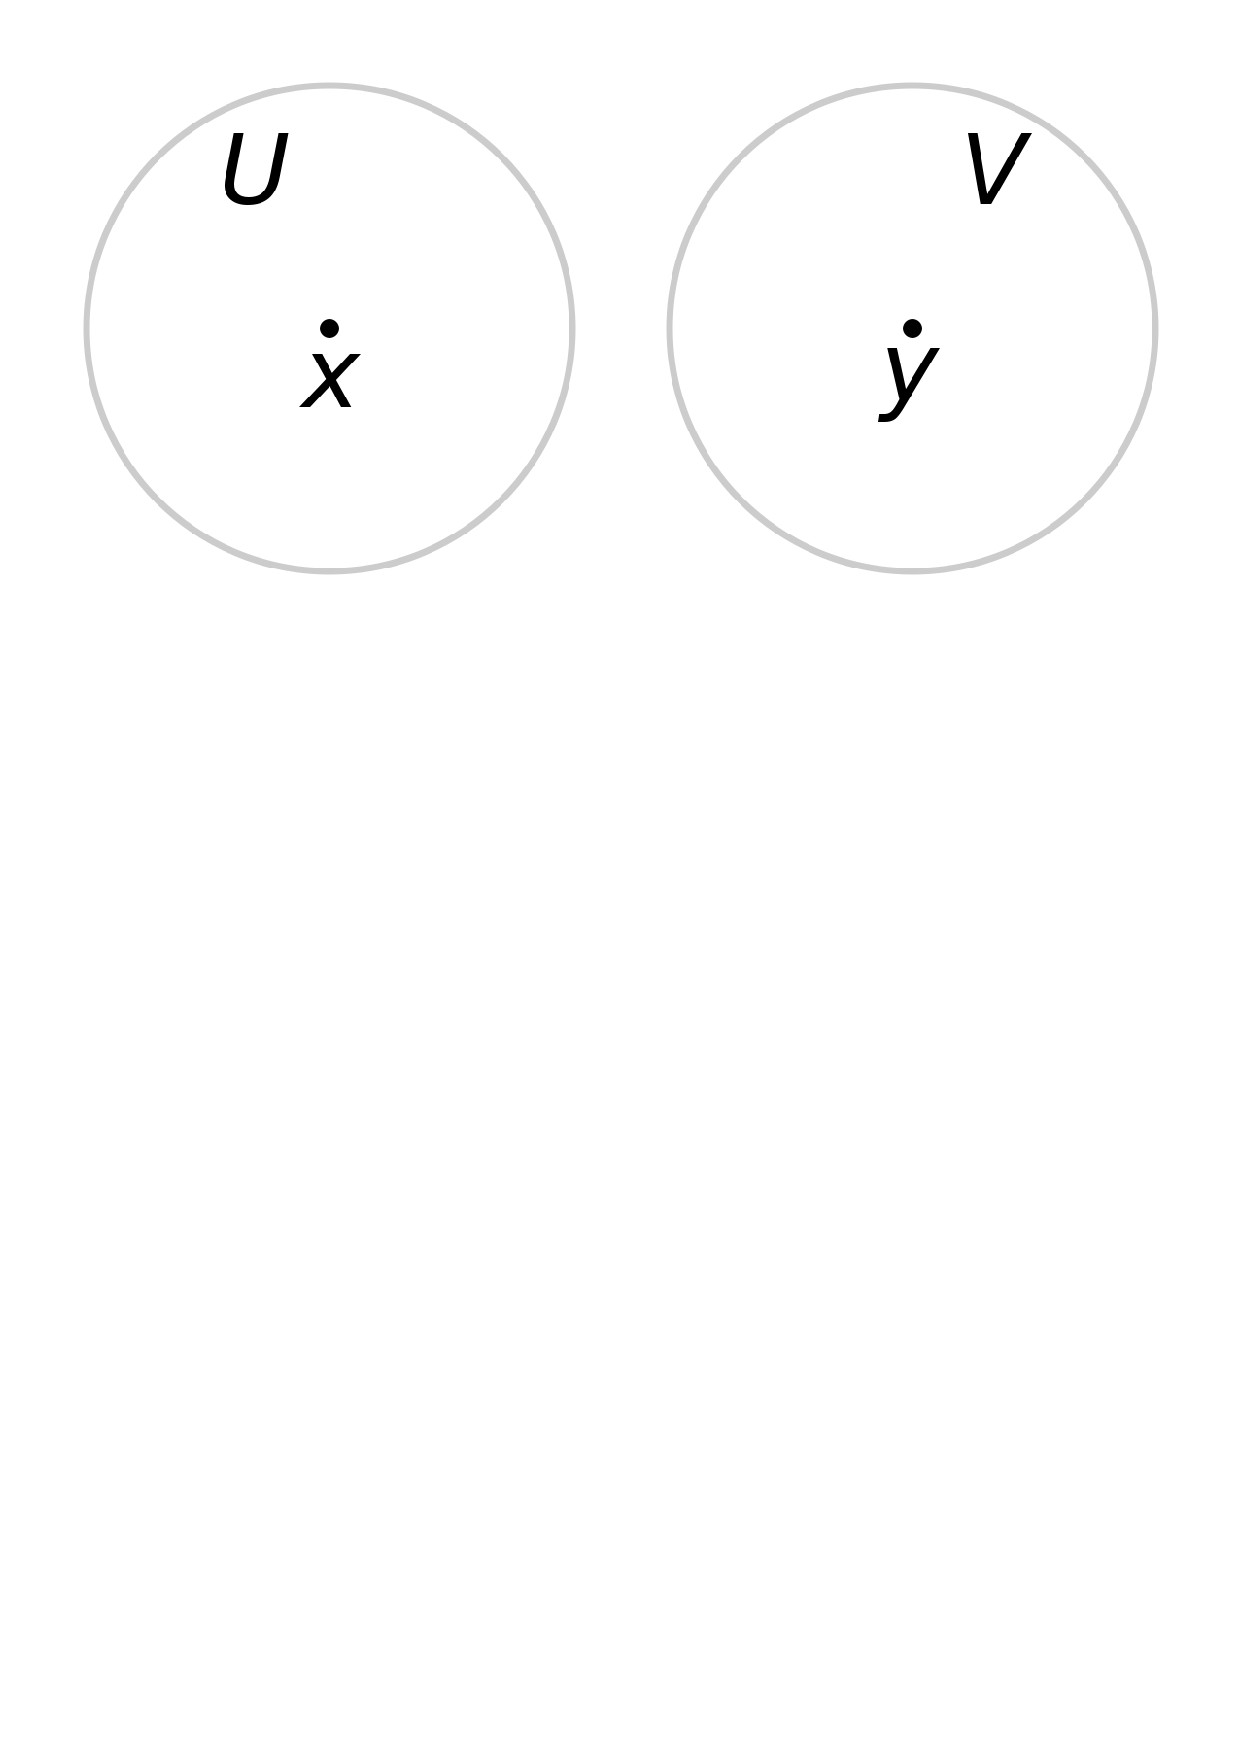
\includegraphics[width=0.75\textwidth]{images/algebra2/hausdorff.pdf}
\end{center}

$\Rightarrow$ F\"ur jedes Primideal $\mathfrak{p}$ von $R$ ist $V(\mathfrak{p}) = \{ \mathfrak{p} \}$

$\Rightarrow$ jedes Primideal in $R$ ist maximales Ideal

$\Rightarrow$ $\dim R = 0$.

\end{Bew}

\end{Folg}

\begin{DefBem}

\begin{enumerate}
\item F\"ur eine beliebige Teilmenge $V$ von $\Spec{R}$ hei\ss t $$\displaystyle I(V) = \bigcap_{\mathfrak{p} \in V} \mathfrak{p}$$ das \emp{Verschwindungsideal}\index{Verschwindungsideal} von $V$.

\item F\"ur jedes Ideal $I$ von $R$ gilt:
$$I(V(I)) = \sqrt{I}$$

\begin{Bew}
Nach \"U7A2d ist $\displaystyle \sqrt{I} = \bigcap_{\substack{\mathfrak{p} \supseteq I \\ \mathfrak{p} \text{ Primideal}}} \mathfrak{p} = \bigcap_{\mathfrak{p} \in V(I)} \mathfrak{p}$
\end{Bew}

\end{enumerate}

\end{DefBem}

\begin{nnFolg}
Ist $V(I_1) = V(I_2)$, so ist $\sqrt{I_1} = \sqrt{I_2}$.
\end{nnFolg}

\begin{DefProp}
\begin{enumerate}
\item Sei $X$ ein topologischer Raum. Eine irreduzible Teilmenge $V \subseteq X$ hei\ss t \emp{irreduzible Komponente}\index{irreduzible Komponente}, wenn $V$ maximale irreduzible Teilmenge ist.

\item Jeder topologischer Raum ist Vereinigung seiner irreduziblen Komponenten.

\item Ist $R$ noethersch, so ist jede abgeschlossene Teilmenge von $V$ von $\Spec{R}$ endliche Vereinigung von irreduziblen Komponenten von $V$; diese sind eindeutig bestimmt.

\end{enumerate}

\begin{Bew}
\begin{enumerate}
\stepcounter{enumi}
\item Zu zeigen: jedes $x \in X$ ist in einer irreduziblen Teilmenge von $X$ enthalten.

Sei $\mathcal{C}_x := \{ U \subseteq X : x \in U, U \text{ irreduzibel} \}$.

$\mathcal{C}_x \neq \emptyset$, da $\{ x \} \in \mathcal{C}_x$.

Seien $(U_i)_{i \in \NN}$ in $\mathcal{C}_x$ mit $U_i \subseteq U_{i+1}$ f\"ur alle $i$.

Sei $U := \bigcup_{i \in \NN} U_i$, zu zeigen: $U \in \mathcal{C}_x$, d.h. $U$ irreduzibel.

\textbf{denn:} Sei $U = V \cup W$, $V,W$ abgeschlossene Teilmengen von $U$. Dann ist $U_i = (U_i \cap V) \cup (U_i \cap W)$ f\"ur jedes $i \in \NN$

Da $U_i$ irreduzibel, ist (\OE) $U_i \cap V = U_i$ f\"ur unendliche viele $i$.

$\Rightarrow$ $U_i \subseteq V$ $\Rightarrow$ $U = \bigcup_{\text{diese }i} U_i \subseteq V$ $\Rightarrow$ $U \subseteq V$.

$\Rightarrow$ $U$ irreduzibel.

Mit dem Zornschen Lemma folgt: $\mathcal{C}_x$ enth\"alt ein maximales Element.

\item \OE\ sei $V = \Spec{R}$: Sei $V = V(I)$ f\"ur ein Ideal $I$.

$V(I) = \{ \mathfrak{p} \in \Spec{R} : I \subseteq \mathfrak{p} \} \overset{\text{bijektiv}}\longleftrightarrow \{ \mathfrak{p'} \in \Spec{R/I} \}$

Aus 2.34b wird folgen: Die Abbildung ist ein Hom\"oomorphismus.

Sei $\mathfrak{V}$ die Menge der abgeschlossenen Teilmengen von $\Spec{R}$, die
\underline{nicht} Vereinigung von endlich vielen irreduziblen Teilmengen sind.
Weiter sei $J := \{ I(V) : V \in \mathfrak{V} \}$.

Zu zeigen: $\mathfrak{V} = \emptyset$.

Anderenfalls ist auch $J \neq \emptyset$. Da $R$ noethersch ist, enth\"alt $J$ ein maximales Element $I(V_0)$ f\"ur ein $V_0 \in \mathfrak{V}$.

$V_0$ ist nicht irreduzibel.

Also gibt es abgeschlossene Teilmengen $V_1, V_2$ von $V_0$ mit $V_0 = V_1 \cup V_2$, $V_1 \neq V_0 \neq V_2$.

$V_i \notin \mathfrak{V}$ f\"ur $i = 1,2$, da $I(V_0) \subsetneqq I(V_i)$

Also lassen sich $V_1$ und $V_2$ als endliche Vereinigung von irreduziblen Teilmengen schreiben.

$\Rightarrow$ $V_0$ l\"asst sich auch als endliche Vereinigung von irreduziblen Teilmengen schreiben. Widerspruch zur Wahl von $V_0$.

$\Rightarrow$ $\mathfrak{V} = \emptyset$.
\bigskip

Sei also $V = V_0 \cup \cdots \cup V_r$ mit irreduziblen Teilmengen $V_i$.

Noch zu zeigen: 
\begin{itemize}
\item die $V_i$ sind (\OE) irreduzible Komponenten.
\item Eindeutigkeit
\end{itemize}

\textbf{denn:}

Aus b) folgt: jedes $V_i$ ist in einer irreduziblen Komponente
$\widetilde{V_i}$ von $V$ enthalten, also $V = \bigcup_{i=0}^r
\widetilde{V_i}$; \OE\ alle $\widetilde{V_i}$ verschieden.

Sei W irreduzible Komponente von $V$.

$\Rightarrow$ $W = \bigcup_{i=0}^r (W \cap \widetilde{V_i})$ $\overset{W \text{ irreduz.}}\Rightarrow$ es gibt ein $i$ mit $W \subseteq \widetilde{V_i}$

$\overset{W \text{ Komponente}}\Rightarrow$ $W = \widetilde{V_i}$.

\end{enumerate}
\end{Bew}

\end{DefProp}

\begin{Folg}
Ein noetherscher Ring hat nur endlich viele minimale Primideale.

\begin{Bew}
Sei $\mathfrak{p} \in \Spec{R}$ minimales Primideal $\Leftrightarrow$ $V(\mathfrak{p}) \subseteq \Spec{R}$ irreduzible Komponente.
\end{Bew}
\end{Folg}

\begin{Prop}
Sei $\alpha : R \rightarrow S$ Ringhomomorphismus.

\begin{enumerate}
\item Die Abbildung $\varphi_\alpha : \Spec{S} \rightarrow \Spec{R}$, $\mathfrak{p} \mapsto \alpha^{-1}(\mathfrak{p})$ ist stetig.

Eleganter: $R \rightarrow \Spec{R}$ ist kontravarianter Funktor
\[
\KatRing \to \KatTop.
\]

\item Ist $\alpha$ surjektiv, so ist $\varphi_\alpha$ injektiv und $\varphi_\alpha(\Spec{S}) = V(\K{\alpha})$.
\end{enumerate}

\begin{Bew}
\begin{enumerate}
\item $\alpha^{-1}(\mathfrak{p})$ ist Primideal:

Seien $a,b \in R$ mit $a \cdot b \in \alpha^{-1}(\mathfrak{p})$ $\Rightarrow$ $\alpha(a \cdot b) \in \mathfrak{p}$ $\overset{\text{\OE}}\Rightarrow$ $\alpha(a) \in \mathfrak{p}$ $\Rightarrow$ $a \in \alpha^{-1}(\mathfrak{p})$

\textbf{$\varphi_\alpha$ stetig}: Zu zeigen: f\"ur jede abgeschlossene Teilmenge $V = V(I)$ von $\Spec{R}$ ist $\varphi_\alpha^{-1}(V)$ abgeschlossen in $\Spec{S}$.

$\varphi_\alpha^{-1}(V(I)) = \{ \mathfrak{p} \in \Spec{S} : I \subseteq
\alpha^{-1}(\mathfrak{p}) \} = \{ \mathfrak{p} \in \Spec{S} : \alpha(I)
\subseteq \mathfrak{p} \} = \{ \mathfrak{p} \in \Spec{S} : \alpha(I) \cdot S
\subseteq \mathfrak{p} \} = V(\alpha(I) \cdot S)$.

\item
Seien $\mathfrak{p}, \mathfrak{p'} \in \Spec{S}$ mit $\varphi_\alpha(\mathfrak{p}) = \varphi_\alpha(\mathfrak{p'})$

$\Rightarrow$ $\alpha^{-1}(\mathfrak{p}) = \alpha^{-1}(\mathfrak{p'})$

$\Rightarrow$ $\alpha(\alpha^{-1}(\mathfrak{p})) = \alpha(\alpha^{-1}(\mathfrak{p'}))$

$\overset{\alpha \text{ surj.}}\Rightarrow$ $\mathfrak{p} = \mathfrak{p'}$.

\end{enumerate}
\end{Bew}
\end{Prop}

\section{Diskrete Bewertungsringe}

\begin{Def} 
Sei $K$ ein Körper.\\
Ein surjektiver Gruppenhomomorphismus $v: K^{\times} \to \ZZ$ heißt
\emp{diskrete Bewertung}\index{Bewertung!diskrete}, wenn für alle $x,y \in
K^{\times}$ mit $x + y \in K^{\times}$ gilt:
$$ v(x+y) \geq \min\{v(x),v(y)\}$$
Anmerkung: Manchmal setzt man $v(0) = \infty$.
\end{Def}

\begin{nnBsp} 
\begin{enumerate}
  \item[1.)] $K = \QQ, \; p \in \ZZ$ Primzahl.\\
  Für $\frac{a}{b} \in \QQ \setminus \{0\}, \; a,b \in \ZZ$
  schreibe $a = p^n \cdot a', \; b = p^m \cdot b'$ mit $p \nmid a',\; p \nmid
  b'$.\\
  Setze $v_p(\frac{a}{b}) \defeqr n - m$.
  $a + b \overset{\text{\OE}: n \leq m}{=} p^n \cdot (a' + p^{m-n} b')$.\\
  $v_p$ heißt p-adische Bewertung\index{Bewertung!p-adische} auf $\QQ$. Es gilt:
  \begin{itemize}
    \item $v_p(a) \geq 0 \; \forall a \in \ZZ$. $v_3(\frac{7}{2}) = 0, \ 
    v_3(\frac{9}{2})= 2$.
    \item $v_p(a+b) = \min\{v_p(a),v_p(b)\}$, falls $v_p(a) \not= v_p(b)$.
  \end{itemize}
  \item[2.)] $K = k(X) = \Quot{k[X]}$ ($k$ Körper).\\
  Für $f = \frac{f_1}{f_2}$ sei $v(f) = v(f_1) - v(f_2)$.
  \begin{enumerate}
    \item $v(f_1) = \ord{a}{f_1}$ für festes $a \in k$
    (Nullstellenordnung).
    Es gilt $v_a(f_1 \cdot f_2) = v_a(f_1) + v_a(f_2)$, 
    $v_a(f_1 + f_2) = v_a((X-a)^{n_1} \cdot g_1 + (X-a)^{n_2} \cdot g_2)
    \overset{\text{\OE}: \; n_1 \leq n_2}{=} v_a((X-a)^{n_1}(g_1 + (X-a)^{n_2 - 
    n_1} \cdot g_2))$.
    \item Für $f \in k[X]$ sei $v(f) = - \deg (f)$.
  \end{enumerate}
\end{enumerate}
\end{nnBsp}

\begin{Bem} 
Sei $v: K^{\times} \to \ZZ$ diskrete Bewertung.
Sei $\rho \in \RR$ mit $0 < \rho < 1$.
Dann ist die Abbildung $|\cdot|_v: K \to \RR, \; |x|_v = \begin{cases}0: & x
= 0 \\\rho^{v(x)}: & x \in K^{\times}\end{cases}$ ein
\emp{Absolutbetrag}\index{Absolutbetrag} auf $K$, d.h. eine Abbildung $K \to
\RR$ mit:
\begin{enumerate}
  \item[(i)] $|x|_v = 0 \Leftrightarrow x = 0$.
  \item[(ii)] $|x \cdot y|_v = |x|_v \cdot |y|_v$.
  \item[(iii)] $|x + y|_v \leq |x|_v + |y|_v$.
\end{enumerate}
In unserer Situation gilt sogar: $|x + y|_v \leq \max\{|x|_v,|y|_v\} \leq |x|_v
+ |y|_v \Rightarrow$ \glqq nichtarchimedischer Betrag\grqq\\
Weiter sei $d(x,y) \defeqr|x - y|$ eine Metrik auf $K$.\\
Kreis hat mehrere Mittelpunkte:\\
Kreis um $a$ mit Radius $r$: $K_r = \{b \in K: d(a,b) \leq r\}$.\\
\textbf{Beh.:} Für jedes $a' \in K_r$ ist $K_r(a') = K_r(a)$.\\
\textbf{Bew.:} Sei $b \in K_r(a)$, also $d(b,a) \leq r$.\\
Dreiecksungleichung: $d(b,a') \leq \max\{\underset{\leq
r}{\underbrace{d(b,a)}},\underset{\leq r}{\underbrace{d(a,a')}}\} \leq r \Rightarrow b \in
K_r(a')$.\\
Es gibt kein allgemeines Dreieck:\\
Ist $d(a,b) < d(a,c)$, also $|a-b| < |c-a|$, so ist $|c-b| = |a-b+c-a| =
\max\{|a-b|,|c-a|\} = |c-a| \Rightarrow$ jedes Dreieck ist gleichschenklig.
\end{Bem}

\begin{Eri}
$\RR$ entsteht aus $\QQ$ durch \glqq Vervollständigung\grqq:\\
$C \defeqr$ Ring der Cauchy-Folgen von $\QQ$ (bzgl. $|\cdot|$)\\
$N \defeqr$ Ideal der Nullfolgen in $C$ (maximales Ideal)\\
$\RR \defeqr C/N$\\
Analog:\\
$C_p \defeqr$ Ring der Cauchy-Folgen von $\QQ$ (bzgl. $|\cdot|_p \defeqr
|\cdot|_{v_p}$)\\
$N_p \defeqr$ Ideal der Nullfolgen in $C_p$ (maximales Ideal)\\
$\QQ_p \defeqr C_p/N_p$ \glqq Körper der $p$-adischen Zahlen\grqq.
\end{Eri}

\begin{Bem}
Ist $v$ diskrete Bewertung auf $K^{\times}$, so ist $\mathcal{O}_v \defeqr \{x
\in K: v(x) \geq 0\} \cup \{0\}$ ein Ring, genauer: ein lokaler Ring mit
maximalem Ideal $\mathfrak{m}_v \defeqr \{ x \in K: v(x) > 0\} \cup \{0\}$.
\end{Bem}

\begin{Bew} 
$\mathcal{O}_v$ ist Ring, da $v(x+y) \geq \min\{v(x),v(y)\} \geq 0$ für alle
$x,y \in \mathcal{O}$.\\
$\mathfrak{m}_v$ ist Ideal: Ist $x \in \mathfrak{m}_v, \; r \in \mathcal{O}_v$, so ist $v(x \cdot r) =
v(x) + v(r) > 0$. Für $x \in \mathcal{O}_v \setminus \mathfrak{m}_v = \{x \in K: v(x) = 0\}$
ist $v(\frac{1}{x})=-v(x)=0 \Rightarrow \frac{1}{x} \in \mathcal{O}_v\setminus
\mathfrak{m}_v \Rightarrow x \in \mathcal{O}_v^{\times}$.
\end{Bew}

\begin{DefProp}
\label{2.38}
\begin{enumerate}
  \item Ein nullteilerfreier Ring $R$ heißt \emp{diskreter
  Bewertungsring}\index{Ring!diskreter Bewertungs-}, wenn es eine diskrete
  Bewertung $v$ von $K = \mathrm{Quot}(R)$ gibt mit $R = \mathcal{O}_v$.
  \item Jeder diskrete Bewertungsring ist noethersch, lokal und eindimensional.
\end{enumerate}
\end{DefProp}

\begin{Bew}
Zeige mehr: $R$ ist Hauptidealring.\\
$R$ ist lokal \chk\\
Sei $m$ das maximale Ideal in $R$.\\
\textbf{Beh.1:} $m$ ist Hauptideal.\\
\textbf{Bew.1:} Sei $t \in R$ mit $v(t)=1 \Rightarrow t \in m$. Sei $x \in m
\setminus\{0\},\; y = \frac{x}{t^{v(x)}} \Rightarrow v(y) - v(t^{v(x)}) = 0
\Rightarrow y \in R^{\times} \Rightarrow x = t^{v(x)} \cdot y \in (t)$.\\
\textbf{Beh.2:} Jedes Ideal $\not= (0)$ in $R$ ist von der Form $m^n$ für ein $n
\geq 0$.\\
\textbf{Bew.2:} Sei $I \subseteq R$ ein Ideal, $n \defeqr \min\{v(x): x \in I
\setminus\{0\}\}$. Sei $x_0 \in I$ mit $v(x_0) = n \Rightarrow
v(\frac{x_0}{t^n})=0 \Rightarrow t^n = \frac{t^n}{x_0} \cdot x_0 \in I
\Rightarrow m^n = (t^n) \subseteq I$.\\
Umgekehrt: $x_0 = t^n \cdot \frac{x_0}{t^n} \in (t^n)$. Sei $x \in I \Rightarrow
v(\frac{x}{t^n})=v(x)-n \geq 0 \Rightarrow x = t^n \cdot \frac{x}{t^n}\in (t^n)$.
\end{Bew}

\begin{Satz} 
\label{Satz12}
Sei $R$ ein lokaler noetherscher Ring der Dimension $1$ mit maximalem Ideal
$\mathfrak{m}$ und Restklassenkörper $k = R/\mathfrak{m}$.\\
Dann sind äquivalent:
\begin{enumerate}
  \item[(i)] $R$ ist diskreter Bewertungsring.
  \item[(ii)] $R$ ist (nullteilerfreier) Hauptidealring.
  \item[(iii)] $R$ ist nullteilerfrei und $\mathfrak{m}$ ist ein Hauptideal.
  \item[(iv)] es gibt ein $t \in R$, sodass jedes $x \in R \setminus \{0\}$ eine.
  eindeutige Darstellung $x=u \cdot t^n$ hat mit $n \in \NN, \; u \in
  R^{\times}$.
  \item[(v)] $\dim[k]{\mathfrak{m}/\mathfrak{m}^2} = 1$.
  \item[(vi)] R ist normal.
\end{enumerate}
\end{Satz}

\begin{Bew} 
\[
  \begin{xy}
    \xymatrix{
       (i) \ar@{=>}[rr]  &                  &  (ii) \ar@{=>}[dl] \ar@{=>}[d] \\
                         & (v) \ar@{=>}[dr] & (vi) \ar@{=>}[d] \\
       (iv) \ar@{=>}[uu] &                  & (iii) \ar@{=>}[ll]
    }
  \end{xy}
\]
\textbf{(i) $\Rightarrow$ (ii):} Prop. \ref{2.38}\\
\textbf{(iv) $\Rightarrow$ (i):} $R$ nullteilerfrei:\\
Annahme: $u \cdot t^n \cdot
v \cdot t^m = 0 = u \cdot v \cdot t^{n+m} \Rightarrow t^{n+m} = t^{n+m} + 0 =
t^{n+m} + u \cdot v \cdot t^{n+m} = (1+u \cdot v) t^{n+m}
\overset{Eind.}{\Rightarrow} 1 + u \cdot v = 1 \Rightarrow u \cdot v = 0
\Rightarrow$ Widerspruch zu $u \cdot v \in R^{\times}$.\\
Diskrete Bewertung:\\
Für $a = u \cdot t^n \in R \setminus \{0\}$ setze $v(a) = n$.
Für $x = \frac{a}{b} \in K = \mathrm{Quot}(R), \; a,b \in R \setminus \{0\}$ setze
$v(x) = v(a) - v(b)$.\\
$v(x)$ wohldefiniert: Ist $x = \frac{a'}{b'}$ mit $a', b' \in R \setminus
\{0\}$, so ist $a \cdot b' =  a' \cdot b$. Aus $a = u \cdot t^n, b = v \cdot
t^m, a' = u' \cdot t^{n'}, b' = v' \cdot t^{m'}$ folgt: $u' \cdot v t^{n'+m} = u
\cdot v' \cdot t^{n + m'} \overset{Eind.}{\Rightarrow} n' + m = n + m'
\Rightarrow n'-m' = n-m$.\\
$v$ ist diskrete Bewertung: $v(x \cdot y) = v (u \cdot t^n \cdot v \cdot
t^m) = v(u \cdot v \cdot t^{n+m}) = n+m = v(x) + v(y)$.
$v(x + y) \overset{m \leq n}{=} v(t^m \cdot (v + u \cdot t^{n-m})) \geq m =
\min\{v(x),v(y)\}$.\\
\textbf{(iii) $\Rightarrow$ (iv):} Sei $\mathfrak{m} = (t)$. Sei $x \in R
\setminus \{0\}$. Da $R$ noethersch ist, ist $\bigcap_{n \geq 0} m^n = (0)$
(Folg. \ref{2.22}).\\
Also gibt es ein (eindeutiges) $n \geq 0$ mit $x \in \mathfrak{m}^n \setminus
\mathfrak{m}^{n+1} \Rightarrow \exists u \in R^{\times}$ mit $x = u \cdot t^n$.
$u$ ist eindeutig: Wäre $u \cdot t^n = v \cdot t^n$, so wäre $(u-v) \cdot t^n =
0$, also $t$ Nullteiler $\Rightarrow$ Widerspruch\\
\textbf{(ii) $\Rightarrow$ (v):} $\mathfrak{m}/\mathfrak{m}^2$ ist
$k$-Vektorraum: $\mathfrak{m}, \mathfrak{m}^2$ und damit
$\mathfrak{m}/\mathfrak{m}^2$ sind $R$-Moduln.
Für $a \in \mathfrak{m}$ und $x \in \mathfrak{m}/\mathfrak{m}^2$ ist $a \cdot
\bar{x} = \overline{a \cdot x} = 0$, da $a \cdot x \in \mathfrak{m}^2
\Rightarrow \bar{a} \cdot \bar{x}$ ist wohldefiniert für die Klasse $\bar{a}$
von $a$ in $R/\mathfrak{m} = k$.\\
Es ist $\mathfrak{m}^2 \not= \mathfrak{m}$, da $\dim R = 1$ (und $R$ noethersch)
$\Rightarrow \dim[k]{\mathfrak{m} / \mathfrak{m}^2} \geq 1$.\\
$\mathfrak{m}/\mathfrak{m}^2$ wird von $\bar{t}$ erzeugt (als $R$-Modul und
damit auch als $R/\mathfrak{m}$-Modul) $\Rightarrow \dim[k]{\mathfrak{m}/
\mathfrak{m}^2} \leq 1 \Rightarrow \dim[k]{\mathfrak{m}/\mathfrak{m}^2} = 1$.\\
\textbf{(v) $\Rightarrow$ (iii):} Sei $t \in \mathfrak{m}$, sodass $\bar{t} \in
\mathfrak{m}/\mathfrak{m}^2$ Erzeuger ist. Mit Nakayama (Folg. \ref{2.21}) folgt:
$t$ erzeugt $\mathfrak{m}$.\\
\textbf{(ii) $\Rightarrow$ (vi):} Jeder (nullteilerfreie) Hauptidealring ist
faktoriell $\Rightarrow R$ ist normal (Bem. \ref{2.10}).\\
\textbf{(vi) $\Rightarrow$ (iii):} Sei $K = \mathrm{Quot}(R)$.\\
Sei $\bar{\mathfrak{m}} \defeqr \{x \in K: x \cdot \mathfrak{m} \subseteq
\mathfrak{m}\}$, $\mathfrak{m}^{-1} \defeqr \{x \in K: x \cdot \mathfrak{m}
\subseteq R\}$\\
Offensichtlich: $R \subseteq \bar{\mathfrak{m}} \subseteq \mathfrak{m}^{-1}$.\\
\textbf{Beh.:} \begin{enumerate}
  \item[1.)] $\bar{\mathfrak{m}} = R$.
  \item[2.)] $\mathfrak{m}^{-1} \not= R$.
  \item[3.)] $\mathfrak{m} \cdot \mathfrak{m}^{-1}=R$ ($\mathfrak{m} \cdot
  \mathfrak{m}^{-1}$ ist das von allen $a \cdot x, \; a \in \mathfrak{m}, \; x
  \in \mathfrak{m}^{-1}$ erzeugte Ideal in $R$).
\end{enumerate}
Dann sei $t \in \mathfrak{m} \setminus \mathfrak{m}^2 \Rightarrow t \cdot
\mathfrak{m}^{-1} \subseteq R$ ist Ideal in $R$.
Wäre $ t \cdot \mathfrak{m}^{-1} \subseteq \mathfrak{m}$, so wäre $(t) = t \cdot
R \overset{3.)}{=} t \cdot \mathfrak{m}^{-1} \cdot \mathfrak{m} \subseteq
\mathfrak{m}^2 \Rightarrow$ Widerspruch zu $t \not\in \mathfrak{m}^2$.
Also ist $t \cdot \mathfrak{m}^{-1} = R$ und $(t) \overset{3.)}{=} t \cdot
\mathfrak{m}^{-1} \cdot \mathfrak{m} = \mathfrak{m}$.\\
\textbf{Bew.3:} Aus $R \subseteq \mathfrak{m}^{-1}$ folgt $\mathfrak{m}
\subseteq \mathfrak{m} \cdot \mathfrak{m}^{-1}$. Wäre $\mathfrak{m} =
\mathfrak{m} \cdot \mathfrak{m}^{-1}$, so wäre $\mathfrak{m}^{-1} \subseteq
\bar{\mathfrak{m}} = R$ im Widerspruch zu Beh. 2.).\\
\textbf{Bew.1:} $\bar{\mathfrak{m}}$ ist Unterring von $K$.\\
Zeige: $\bar{\mathfrak{m}}$ ist ganz über $R$ (dann ist $\bar{\mathfrak{m}} =
R$, da $R$ normal).\\
Es genügt zu zeigen: $\bar{\mathfrak{m}}$ ist endlich erzeugter $R$-Modul.\\
Für $t \in \mathfrak{m} \setminus \{0\}$ ist $t \cdot \bar{\mathfrak{m}}
\subseteq R$, also endlich erzeugt, da $R$ noethersch.
Als $R$-Modul sind $\bar{\mathfrak{m}}$ und $t \cdot \bar{\mathfrak{m}}$
isomorph.\\
\textbf{Bew.2:} Sei $t \in \mathfrak{m} \setminus\{0\}$.\\
\textbf{Beh.4:} Es gibt ein $n \geq 1$ mit $\mathfrak{m}^n \subseteq (t)$.\\
Sei $n$ in Beh.4 minimal, $y \in \mathfrak{m}^{n-1} \setminus (t), \; x \defeqr
\frac{y}{t} \in K$.
Dann ist $x \in \mathfrak{m}^{-1}: x \cdot \mathfrak{m} = \frac{y}{t} \cdot
\mathfrak{m} \subseteq \frac{1}{t} \cdot \mathfrak{m}^n \subseteq R$, aber $x
\not\in R$, sonst wäre $y = x \cdot t \in (t) \Rightarrow$ Widerspruch.\\
\textbf{Bew.4:} $\sqrt{(t)} = \bigcap_{\mathfrak{p} \subset R, t \in
\mathfrak{p}} \mathfrak{p} = \mathfrak{m}$.\\
Seien $x_1, \dots, x_r$ Erzeuger von $\mathfrak{m}, \; \nu_i \in \NN
\;(i=1, \dots,r)$ mit $x_i^{\nu_i} \in (t)$.\\
Für $n = 1 + \sum_{i =1}^r(\nu_i -1)$ ist dann $\mathfrak{m}^n \subseteq (t)$,
da $\mathfrak{m}^n$ erzeugt wird von den $x_1^{\nu_1} \cdot \ldots \cdot
x_r^{\nu_r}$ mit $\sum \nu_i = n$.
\end{Bew}

\begin{nnBsp}
$R = (k[X,Y]/(Y^2-X^3-X^2))_{(X,Y)}$ ist nullteilerfrei, eindimensional, lokal, noethersch aber kein diskreter Bewertungsring.\\
Denn: das maximale Ideal in $R$ ist kein Hauptideal: $\mathfrak{m}=(X,Y), \; f = Y^2-X^2(X+1) \in \mathfrak{m}^2$.\\
Es gilt $\dim[k]{\mathfrak{m}/\mathfrak{m}^2} = 2$, da $X,Y$ linear unabhängig in $\mathfrak{m}/\mathfrak{m}^2$.
Sei $\mathfrak{M}$ das von $X$ und $Y$ in $k[X,Y]$ erzeugte Ideal.
$\mathfrak{m}/\mathfrak{m}^2 = (\mathfrak{M}/(f))/(\mathfrak{M}^2/(f)) \cong \mathfrak{M}/\mathfrak{M}^2$\\
Geometrisch:\\
$V(f) = \{(x,y) \in k^2: \; f(x,y) = 0\}$\\
Singularität in $(0,0) = (X,Y) \Rightarrow$ \glqq Newton-Knoten\grqq.
\begin{center}
	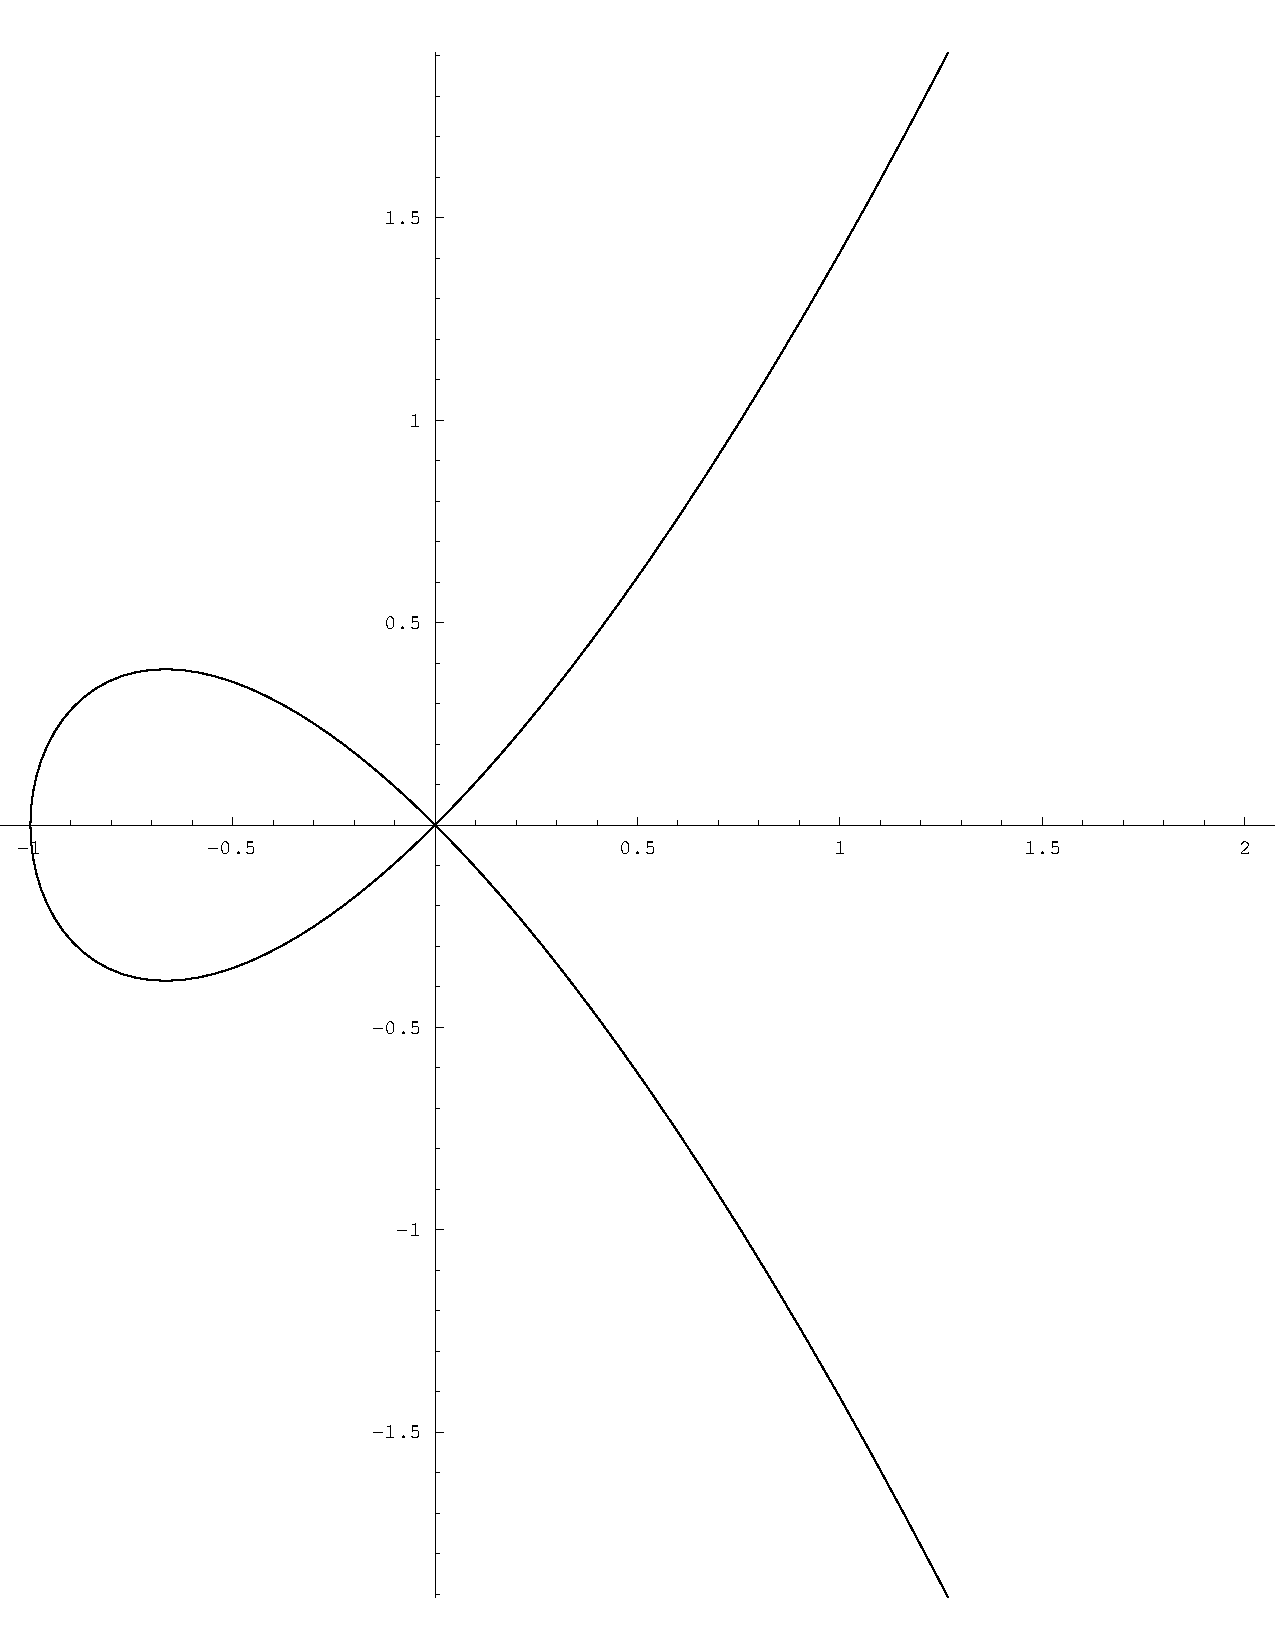
\includegraphics[width=0.75\textwidth]{images/algebra2/newtonknoten.pdf}
\end{center}
\end{nnBsp}

\section{Dedekindringe}

\begin{Def}

Ein nullteilerfreier Ring hei"st \emp{Dedekindring}\index{Dedekindring}, wenn er noethersch, normal und eindimensional ist.

\begin{nnBsp}
\begin{enumerate}
\item[1)] $\ZZ$, $k[X]$ ($k$ K\"orper).

\item[2)] diskrete Bewertungsringe.

\item[3)] (nullteilerfreie) Hauptidealringe, die kein Körper sind.

\item[4)] der ganze Abschluss $\mathcal{O}_d$ von $\ZZ$ in $\QQ(\sqrt{d})$ wobei $d \in \ZZ$ quadratfrei.

$\mathcal{O}_d = \begin{cases}
\ZZ[\sqrt{d}] & d \not\equiv 1 \mod 4\\
\ZZ[\frac{1+\sqrt{d}}{2}] & d \equiv 1 \mod 4
\end{cases}$

\end{enumerate}
\end{nnBsp}

\end{Def}

Beobachtung: Es gibt Dedekindringe, die nicht faktoriell sind: Beispiel:
$\ZZ[\sqrt{-5}]$. ($2 \cdot 3 = (1 + \sqrt{-5}) (1 - \sqrt{-5})$.

\begin{DefBem}
Sei $R$ nullteilerfrei, $K = \Quot{R}$.
\begin{enumerate}
\item Ein $R$-Untermodul $I \neq (0)$ von $K$ hei"st \emp{gebrochenes Ideal}\index{Ideal!gebrochenes} von $R$, wenn es ein $a \in R \setminus \{0\}$ gibt mit $a \cdot I \subseteq R$.

\item F\"ur gebrochene Ideale $I,J$ von $R$ sei $I \cdot J$ der von allen $a \cdot b$, $a \in I, b \in J$, erzeugte $R$-Untermodul von $K$.

\item Die gebrochnenen Ideale von $R$ bilden mit der Multiplikation aus b) ein kommutatives Monoid mit neutralem Element $R$.

\item Die Einheiten in diesem Monoid hei"sen \emp{invertierbare} (gebrochene) Ideale.

d.h. $I$ invertiertbar $\Leftrightarrow$ $\exists I'$ mit $I \cdot I' = R$.

\end{enumerate}
\end{DefBem}

\begin{nnBsp}
\begin{enumerate}
\item[1)] Jeder endlich erzeugbare $R$-Untermodul von $K$ ist gebrochenes Ideal.

\textbf{denn:} Seien $x_1 = \frac{a_1}{b_1}, \ldots, x_n = \frac{a_n}{b_n}$ Erzeuger von $M$ ($a_i, b_i \in R$) $\Rightarrow$ f\"ur $b = b_1 \cdot \ldots \cdot b_n$ ist $b \cdot M \subseteq R$.

\item[2)] Ist $I$ gebrochenes Ideal, so ist $I^{-1} := \{ x \in K : x \cdot I \subseteq R \}$ ebenfalls gebrochenes Ideal: f\"ur jedes $a \in I$ ist $a \cdot I^{-1} \subseteq R$.

$I$ ist invertierbar $\Leftrightarrow$ $I \cdot I^{-1} = R$.

\item[3)] $R = k[X,Y]$, $I = (X,Y)$ $\Rightarrow$ $I^{-1} = R$.

\textbf{denn:} f\"ur $a = \frac{f}{g} \in I^{-1}$ muss gelten: $a \cdot X \in R$, $a \cdot Y \in R$.

\item[4)] Jedes Hauptideal $\neq (0)$ ist invertierbar: $(a) \cdot (\frac{1}{a} \cdot R) = R$.
\end{enumerate}
\end{nnBsp}

\begin{Bem}\label{2.41}
Jedes invertierbare Ideal in einem Integrit\"atsbereich ist endlich erzeugbar (als $R$-Modul).

\begin{Bew}
Sei $I$ invertierbar, also $I \cdot I^{-1} = R$, dann gibt es $a_i \in I, b_i \in I^{-1}$ mit $1 = \sum_{i=1}^{n} a_i b_i$

\textbf{Beh:} $a_1, \ldots a_n$ erzeugen $I$.

\textbf{denn:} Sei $a \in I$ $\Rightarrow$ $a = a \cdot 1 = a \cdot \sum_{i=1}^{n} a_i b_i = \sum_{i=1}^{n} a_i \underbrace{(a b_i)}_{\in R}$.

\end{Bew}
\end{Bem}

\begin{Satz}\label{Satz13}
F\"ur einen nullteilerfreien Ring $R$ sind \"aquivalent:

\begin{enumerate}
\item[(i)] $R$ ist Dedekindring oder K\"orper.

\item[(ii)] $R$ ist noethersch und $R_\mathfrak{p}$ ist diskreter Bewertungsring f\"ur jedes Primideal $\mathfrak{p} \neq (0)$ in $R$.

\item[(iii)] Jedes Ideal $I \neq (0)$ in $R$ ist invertierbar.

\item[(iv)] Die gebrochenen Ideale in $R$ bilden eine Gruppe.

\item[(v)] Jedes echte Ideal in $R$ ist Produkt von endlich vielen Primidealen.

\item[(vi)] Jedes echte Ideal besitzt ein eindeutige Darstellung als Produkt von endlich vielen Primidealen.
\end{enumerate}

\end{Satz}

\begin{Bew}

\textbf{Beweisplan:}
\[
\begin{xy}
\xymatrix{
			     & (ii) \ar@{=>}[dr] &                                & (v) \ar@{<=>}[dd] \\
(i) \ar@{=>}[ur] &                   & (iii) \ar@{=>}[dl] \ar@{<=>}[ur] \\
                 & (iv) \ar@{=>}[ul] &                              & (vi) 
}
\end{xy}
\]

\begin{description}
\item[(i) $\Rightarrow$ (ii)]:

Sei $\mathfrak{p} \neq (0)$ Primideal im Dedekindring $R$ $\Rightarrow$ $R_\mathfrak{p}$ noethersch, $\dim{R_\mathfrak{p}} = \hoe{\mathfrak{p}} = 1$, da $\dim R = 1$.

$R_\mathfrak{p}$ normal: Sei $a \in K = \Quot{R} = \Quot{R_\mathfrak{p}}$ ganz \"uber $R_\mathfrak{p}$.

Dann gibt es eine Gleichung: $a^n + \sum_{i=0}^{n-1} \frac{b_i}{s_i} a^i = 0$ mit $b_i \in R, s_i \in R \setminus \mathfrak{p}$

$\Rightarrow$ $(s \cdot a)^n + \sum_{i=0}^{n-1} \widetilde{b_i} (s a)^i = 0$ mit $\widetilde{b_i} \in R$, $s := \prod_{i=0}^{n-1} s_i$

$\overset{R \text{ normal}}{\Rightarrow}$ $s \cdot a \in R$ $\Rightarrow$ $a
\overset{s \notin \mathfrak{p}}{=} \frac{s \cdot a}{s} \in R_\mathfrak{p}$.

\item[(iii) $\Rightarrow$ (iv)]:

Sei $(0) \neq I \subset K$ gebrochenes Ideal, $a \in R \setminus \{0\}$ mit $a
\cdot I \subseteq R$ $\overset{(iii)}{\Rightarrow}$ $a \cdot I$ invertierbar 
$\Rightarrow$ $R = (a \cdot I) \cdot I' = I \cdot (a \cdot I')$ $\Rightarrow$ $I$ ist invertierbar.

\item[(ii) $\Rightarrow$ (iii)]:

Sei $I \neq (0)$ Ideal in $R$. $K = \Quot{R}$, $I^{-1} := \{ x \in K : x \cdot
I \subseteq R \}$
	
Zu zeigen: $I \cdot I^{-1} = R$.

Annahme: $I \cdot I^{-1} \subsetneqq R$:\\
Dann gibt es ein maximales Ideal $\mathfrak{m}$ von $R$ mit $I \cdot I^{-1} \subseteq \mathfrak{m}$.\\
$\Rightarrow$ $R_\mathfrak{m}$ ist diskreter Bewertungsring.\\
$\Rightarrow$ $I \cdot R_\mathfrak{m}$ ist Hauptideal, d.h. $I \cdot R_\mathfrak{m} = \frac{a}{s} \cdot R_\mathfrak{m}$ f\"ur ein $a \in I, s \in R \setminus \mathfrak{m}$

Seien $b_1, \ldots, b_n \in I$ Erzeuger ($R$ ist noethersch) $\Rightarrow$
$\frac{b_i}{1} = \frac{a}{s} \cdot \frac{r_i}{s_i}$ f\"ur gewisse $r_i \in R,
s_i \in R \setminus \mathfrak{m}$.

Sei $t = s \cdot \prod_{i=1}^{n} s_i$. Es gilt: $t \in R \setminus \mathfrak{m}$.

F\"ur jedes $i = 1, \ldots n$ ist $\frac{t}{a} \cdot b_i = r_i \cdot s_1 \cdot \ldots \cdot \widehat{s_i} \cdot \ldots \cdot s_n \in R$.

$\Rightarrow$ $\frac{t}{a} \in I^{-1}$ $\Rightarrow$ $t = a \cdot \frac{t}{a} \in I \cdot I^{-1} \subseteq \mathfrak{m}$. Widerspruch.

\item[(iv) $\Rightarrow$ (i)]:

\underline{$R$ noethersch}: Nach Bemerkung \ref{2.41} ist jedes invertierbare Ideal endlich erzeugbar.

\underline{$R$ normal}: Sei $x \in K$ ganz \"uber $R$ $\Rightarrow$ $R[x]$ ist
endlich erzeugbarer $R$-Modul, also gebrochenes Ideal (Beispiel $1$) $\overset{(iv)}{\Rightarrow}$ $R[x]$ ist invertierbar. 

Da $R[x]$ Ring ist, gilt $R[x] \cdot R[x] = R[x]$ $\overset{R[x]\text{ invertierbar}}{\Rightarrow}$ $R[x] = R$ (neutrale Element)
$\Rightarrow$ $x \in R$.

\underline{$\dim R \leq 1$}: Sei $\mathfrak{p} \neq (0)$ Primideal in $R$, $\mathfrak{m} \subseteq R$ maximales Ideal mit $\mathfrak{p} \subseteq \mathfrak{m}$.

$\Rightarrow$ $\mathfrak{m}^{-1} \cdot \mathfrak{p} \subseteq \mathfrak{m}^{-1} \mathfrak{m} \overset{(iv)}{=} R$ und $\mathfrak{m} \cdot (\mathfrak{m}^{-1} \mathfrak{p}) = \mathfrak{p}$.

$\overset{\mathfrak{p}\text{ Primideal}}{\Rightarrow}$ $\mathfrak{m} = \mathfrak{p}$ oder $\mathfrak{m}^{-1} \mathfrak{p} \subseteq \mathfrak{p}$.

Falls $\mathfrak{m}^{-1} \mathfrak{p} \subseteq \mathfrak{p}$ $\overset{\cdot \mathfrak{p}^{-1}}{\Rightarrow}$ $\mathfrak{m}^{-1} \subseteq R$. Widerspruch (da sonst $\mathfrak{m}^{-1} \cdot \mathfrak{m} \subseteq \mathfrak{m}$).

\item[(iii) $\Rightarrow$ (v)]:

Sei $I \neq (0)$ echtes Ideal in $R$.

Setze $I_0 := I$.

Definiere induktiv: $I_n$ f\"ur $n \geq 1$:

Ist $I_{n-1} \neq R$, so sei $\mathfrak{m}_{n-1}$ maximales Ideal mit $I_{n-1} \subseteq \mathfrak{m}_{n-1}$ und $I_n := I_{n-1} \mathfrak{m}_{n-1}^{-1} \subseteq R$.

Es ist $I_{n-1} \subseteq I_n$.

W\"are $I_n = I_{n-1}$, so w\"are $\mathfrak{m}_{n-1}^{-1} = R$. Widerspruch zu $\mathfrak{m}_{n-1}^{-1} \cdot \mathfrak{m}_{n-1} = R$.

Da nach \ref{2.41} $R$ noethersch ist, wird die Kette $I_0 \subsetneqq I_1 \subsetneqq I_2 \subsetneqq \cdots$ station\"ar

$\Rightarrow$ $\exists n$ mit $R = I_n = I_{n-1} \mathfrak{m}_{n-1}^{-1} = I_{n-2} \mathfrak{m}_{n-2}^{-1} \mathfrak{m}_{n-1}^{-1} = \cdots = I_0 \cdot \prod_{i=0}^{n-1} \mathfrak{m}_{i}^{-1}$

$\Rightarrow$ $I = I_0 = \prod_{i=0}^{n-1} \mathfrak{m}_i$.

\item[(v) $\Rightarrow$ (vi)]:

Sei $\mathfrak{p}_1 \cdots \mathfrak{p}_n = \mathfrak{q}_1 \cdots \mathfrak{q}_m$ mit Primidealen $\mathfrak{p}_i$, $\mathfrak{q}_i$. Zu zeigen: $n=m$ und $\mathfrak{p}_i = \mathfrak{q}_{\sigma(i)}$ f\"ur eine Permutation $\sigma \in S_n$:

Induktion \"uber $n$:

$n=1$: $\mathfrak{p} = \mathfrak{p}_1 = \mathfrak{q}_1 \cdots \mathfrak{q}_m$ $\overset{\mathfrak{p}\text{ prim}}{\Rightarrow}$ $\exists i_0$ mit $\mathfrak{q}_{i_0} \subseteq \mathfrak{p}$. Umgekehrt ist $\mathfrak{p} \subseteq \mathfrak{q}_i$ f\"ur jedes $i$ $\Rightarrow$ $\mathfrak{p} = \mathfrak{q}_{i_0}$

$n>1$: \OE\  $\mathfrak{p}_1$ minimal bzgl. $\subseteq$ in $\{ \mathfrak{p}_1,
\ldots \mathfrak{p}_n \}$.

Aus $\prod \mathfrak{q}_i \subseteq \prod \mathfrak{p}_j \subseteq \mathfrak{q}_{i_0}$ $\Rightarrow$ $\exists j_0$ mit $\mathfrak{p}_{j_0} \subseteq \mathfrak{q}_{i_0} \subseteq \mathfrak{p}_1$ $\overset{\mathfrak{p}_1\text{ minimal}}{\Rightarrow}$ $\mathfrak{p}_1 = \mathfrak{q}_{i_0}$ $\overset{(iii)}{\Rightarrow}$ $\mathfrak{p}_2 \cdots \mathfrak{p}_n = \mathfrak{q}_1 \ldots \widehat{\mathfrak{q}_{i_0}} \ldots \mathfrak{q}_m$ $\Rightarrow$ Behauptung aus IV.

\item[(v) $\Rightarrow$ (iii)]:

Sei $I \neq (0)$, $I = \mathfrak{p}_1 \cdots \mathfrak{p}_r$ mit Primidealen
$\mathfrak{p}_i$. Ist jedes $\mathfrak{p}_i$ invertierbar, so ist $I^{-1} =
\mathfrak{p}_1^{-1} \cdots \mathfrak{p}_r^{-1}$ und $I \cdot I^{-1} = R$. Also
\OE\  $I = \mathfrak{p}$ Primideal.

Sei $a \in \mathfrak{p}\setminus \{0\}$, $(a) = \mathfrak{q}_1 \cdots \mathfrak{q}_n$ mit Primidealen $\mathfrak{q}_i$ $\Rightarrow$ $\mathfrak{q}_i \subseteq \mathfrak{p}$ f\"ur ein $i$.

$\mathfrak{q}_i$ ist invertierbar: $\mathfrak{q}_i^{-1} = \frac{1}{a} \cdot R \cdot \mathfrak{q}_1 \cdots \widehat{\mathfrak{q}_i} \cdots \mathfrak{q}_n$

Es gen\"ugt also zu zeigen: $\mathfrak{q}_i = \mathfrak{p}$

\textbf{Beh. 1} Jedes invertierbare Primideal $\mathfrak{q}$ in $R$ ist maximal.

\textbf{Bew. 1}
Ist $\mathfrak{q}$ nicht maximal, so sei $x \in R \setminus \mathfrak{q}$ mit $\mathfrak{q} + (x) \neq R$.

\textbf{Beh. 2} Dann ist $(\mathfrak{q} + (x))^2 = \mathfrak{q} + (x^2)$

Dann ist
\[
\mathfrak{q} \subseteq \mathfrak{q} + (x^2) \overset{\text{Beh. 2}}{=}
(\mathfrak{q} + (x))^2 \subseteq \mathfrak{q}^2 + (x).\quad(\ast)
\]

Weiter ist $\mathfrak{q} \subseteq \mathfrak{q}^2 + \mathfrak{q} \cdot (x)$

\textbf{denn:} Sei $b \in \mathfrak{q}$, schreibe nach $(\ast)$ $b = c + r x$ mit $c \in \mathfrak{q}^2, r \in R$, dabei ist $r \in \mathfrak{q}$, da $r \cdot x \in \mathfrak{q}$ und $x \notin \mathfrak{q}$.

$\Rightarrow$ $\mathfrak{q} = \mathfrak{q}^2 + \mathfrak{q} \cdot (x)$ (\glqq$\supseteq$\grqq\ ist trivial)

$\Rightarrow$ $\mathfrak{q} = \mathfrak{q} (\mathfrak{q} + (x)) \overset{\mathfrak{q}\text{ invertierbar}}\Rightarrow R = \mathfrak{q} + (x)$ Widerspruch.

\textbf{Bew 2.} \glqq$\subseteq$\grqq\ \chk, \glqq$\supseteq$\grqq:

Schreibe beide Seiten als Produkt von Primidealen.

$\mathfrak{q} + (x) = \mathfrak{p}_1 \cdots \mathfrak{q}_r$, $\mathfrak{q} + (x^2) = \mathfrak{q}_1 \cdots \mathfrak{q}_s$.

In $R / \mathfrak{q}$ ist dann: $(\bar{x}) = \overline{\mathfrak{p}_1} \cdots \overline{\mathfrak{p}_r}$, $(\bar{x})^2 = \overline{\mathfrak{q}_1} \cdots \overline{\mathfrak{q}_s} = \overline{\mathfrak{p}_1^2} \cdots \overline{\mathfrak{q}_r^2}$

$(\bar{x}), (\bar{x}^2)$ invertierbar $\Rightarrow$ $\overline{\mathfrak{p}_i}, \overline{\mathfrak{q}_j}$ invertierbar.

$\overset{\text{\glqq(iii) + (v) = (vi)\grqq}}{\Rightarrow}$
$\overline{\mathfrak{q}_o} = \overline{\mathfrak{p}_{\sigma(i)}^2}$
$\Rightarrow$ \OE\  $\mathfrak{q}_i = \mathfrak{p}_i^2$.

\end{description}
\end{Bew}

\begin{Satz} 
Sei $R$ ein Dedekindring, $K = \Quot{R}, \; L/K$ endliche separable
Körpererweiterung.
$S$ der ganze Abschluss von $R$ in $L$.\\
Dann ist $S$ ein Dedekindring.
\end{Satz}

\begin{Bew} 
$\dim S=1:$ Folgt aus Satz~\ref{Satz10}\ref{Satz10c}.\\
$S$ normal:\\
Sei $x\in L$ ganz über $S$, also $x^n+\sum_{i=1}^{n-1}a_i x^i = 0$ mit $a_i \in S$.
Sei $S'$ der von $R$ und $a_1,\dots,a_{n-1}$ erzeugte Unterring von $S$.
$S'$ ist endlich erzeugbarer $R$-Modul, da die $a_i$ ganz über $R$ sind.
$S'[x]$ ist endlich erzeugter $S'$-Modul und damit endlich erzeugbarer $R$-Modul $\Rightarrow x$ ist ganz über $R \Rightarrow x \in S$.\\
$S$ noethersch:\\
\textbf{Beh.1:} Es gibt ein primitives Element $\alpha$ von $L/K$ mit $\alpha \in S$.\\
\textbf{Bew.1:} Sei $\tilde{\alpha} \in L$ primitives Element, also $1, \tilde{\alpha}, \tilde{\alpha}^2, \dots, \tilde{\alpha}^{n-1}$ ist $K$-Basis von $L \; (n \defeqr [L:K])$.
Sei $\tilde{\alpha}^n = \sum_{i=0}^{n-1} c_i \tilde{\alpha}^i$ für gewisse $c_i \in K, \; i = 0, \dots, n-1$.
Schreibe $c_i = \frac{a_i}{b_i}$ mit $a_i, b_i \in R, \; b \defeqr \prod_{i=0}^{n-1} b_i$.
Setze $\alpha \defeqr b \cdot \tilde{\alpha} \Rightarrow \alpha^n = b^n \cdot
\sum_{i=0}^{n-1} c_i \tilde{\alpha}^i = \sum_{i=0}^{n-1} \underset{\in
R}{\underbrace{c_i b^{n-i}}}\alpha^i \Rightarrow \alpha \in S$.\\
$1, \alpha, \alpha^2, \dots, \alpha^{n-1}$ linear unabhängig:\\
Sei $\sum_{i=0}^{n-1} \lambda_i \alpha^i = 0 \Rightarrow \sum \lambda_i b^i
\tilde{\alpha}^i = 0 \Rightarrow \lambda_i b^i = 0 \; \forall i$.\\
Sei nun $\bar{K}$ ein algebraischer Abschluss von K.
Seien $\sigma_1, \dots, \sigma_n$ die verschiedenen Einbettungen von $L$ in
$\bar{K}$, also die Elemente von $\Hom[K]{L}{\bar{K}}$.\\
$d \defeqr d(\alpha) \defeqr (\det(\sigma_i(\alpha^{j-1})_{i,j=1, \dots, n}))^2$
heißt die Diskriminante\index{Diskriminante} von $L/K$ (bzgl. $\alpha$).\\
\textbf{Beh.2:}
\begin{enumerate} 
  \item $d \not= 0$.
  \item $S$ ist in dem von $\frac{1}{d}, \frac{\alpha}{d}, \dots,
  \frac{\alpha^{n-1}}{d}$ erzeugten $R$-Untermodul von $L$ enthalten.
\end{enumerate}
Dann ist $S$ als Untermodul eines endlich erzeugbaren $R$-Modul selbst endlich
erzeugbar und damit noethersch (weil $R$ noethersch ist).\\
\textbf{Bew.2:}
\begin{enumerate}
  \item
  \[
  d = \det
  \begin{pmatrix}
  1 & 1 & \dots & 1 \\
  \sigma_1(\alpha) & \sigma_2(\alpha) & \dots & \sigma_n(\alpha) \\
  \sigma_1(\alpha)^2 & \sigma_2(\alpha)^2 & \dots & \sigma_n(\alpha)^2 \\
  \vdots & \vdots & \ddots & \vdots \\
  \sigma_1(\alpha)^{n-1} & \sigma_2(\alpha)^{n-1} & \dots & \sigma_n(\alpha)^{n-1}
  \end{pmatrix}
\]
\[
  \overset{\text{\scriptsize Vandermonde}}{=}(-1)^n \prod_{i \not= j}
  (\sigma_i(\alpha) - \sigma_j(\alpha)) \not= 0
\]
  \item Für $x \in L$ sei Sp$(x) \defeqr \sum_{i=1}^n \sigma_i(x) \in \bar{K}$
  (\glqq Spur\grqq)\\
  Sp$(x) \in K:$ Für $\sigma \in \Aut[K]{\bar{K}}$ ist $\sigma \circ \sigma_i \in
  \Hom[K]{L}{\bar{K}}$\\
  $\sigma(\Sp(x)) = \sum_{i=1}^n (\sigma \circ \sigma_i)(x) = \Sp(x)
  \in \bar{K}^{\Aut[K]{\bar{K}}} = K$.\\
  Sei $x \in S, \; x = \sum_{j=1}^n c_j \alpha^{j-1}$ mit $c_j \in K$.\\
  \textbf{Beh.3:} $c = \begin{pmatrix} c_1\\ \vdots\\ c_n \end{pmatrix}$ ist
  Lösung eines LGS $A \cdot c = b$ mit $b \in R^n$ und $A \in R^{n \times n}$
  mit $\det A = d$.\\
  Nach der Cramerschen Regel ist dann $c_i = \frac{\det A_i}{\det A}$ wobei
  $A_i$ aus $A$ dadurch entsteht, dass die $i$-te Zeile durch $b$ ersetzt wird.
  $\Rightarrow c_i \in \frac{1}{d}R \Rightarrow x$ liegt in dem von $\frac{1}{d}, \frac{\alpha}{d}, \dots,
  \frac{\alpha^{n-1}}{d}$ erzeugten $R$-Modul.
\end{enumerate}
\textbf{Bew.3:} Für $i=1, \dots, n$ ist
\[
\Sp(\alpha^{i-1} x) = \sum_{j=1}^n
\Sp((\alpha^{i-1}\alpha^{j-1})c_j) \in K \quad (*)
\]
ganz über $R
\Rightarrow \Sp(\alpha^{i-1}x) \in R \Rightarrow A \defeqr
(\Sp(\alpha^{i-1} \alpha^{j-1})_{i,j = 1, \dots, n}) \in R^{n \times n}$.\\
$b \defeqr \begin{pmatrix} \Sp(x)\\ \Sp(\alpha x)\\ \vdots \\
\Sp(\alpha^{n-1}x) \end{pmatrix} \in R^n$, $(*)$ heißt $A \cdot c = b$.\\
Noch zu zeigen: $\det A = d$.\\
Nach Definition ist $d = (\det B)^2$ mit $B = (\sigma_i(\alpha^{j-1})_{i,j})
\Rightarrow B^T \cdot B = (\beta_{ij})$ mit $\beta_{ij} = \sum_{k=1}^n
\sigma_k(\alpha^{i-1}) \sigma_k(\alpha^{j-1}) = \Sp(\alpha^{i-1}
\alpha^{j-1}) \Rightarrow B^T \cdot B = A \Rightarrow \det A = (\det B)^2 =
d$
\end{Bew}

\begin{nnBsp}
$K=\QQ$, $L=\QQ(\sqrt{D})$, $D$ quadratfrei, $R=\ZZ$.

Was ist $d$? $\alpha = \sqrt{D}$, $\varsigma_1=\id$, $\varsigma_2(a+b\sqrt{D})=a-b\sqrt{D}$

$B=\left(\begin{array}{cc}1&1\\\sqrt{D}&-\sqrt{D}\end{array}\right)$

$d=\det(B)^2=(-2\sqrt{D})^2=4D$.

\end{nnBsp}

\section{Primärzerlegung}

\begin{nnBsp}
$R = k[X,Y]$. $I = (X^2, Y)$ hat keine Darstellung als Produkt von Primidealen.

\textbf{denn}: Wäre $I = \mathfrak{p}_1^{\nu_1} \cdots \mathfrak{p}_r^{\nu_r}$ mit paarweise verschiedenen Primidealen $\mathfrak{p}_i$, so wäre $\sqrt{I} = \mathfrak{p}_1 \cdots \mathfrak{p}_r = (X,Y) = \mathfrak{m}$, also $r = 1$, $\mathfrak{p}_1 = \mathfrak{m}$. Aber: $\mathfrak{m} \supsetneqq I \supsetneqq \mathfrak{m}^2$.

\end{nnBsp}

\begin{DefBem}
Sei $R$ Ring, $\mathfrak{q} \subseteq R$ echtes Ideal.

\begin{enumerate}
\item $\mathfrak{q}$ heißt \emp{Primärideal}\index{Primärideal}, wenn für alle $a,b \in R$ mit $a \cdot b \in \mathfrak{q}$ und $a \notin \mathfrak{q}$ gilt: es gibt ein $n \geq 1$ mit $b^n \in \mathfrak{q}$.

\item Ist $\mathfrak{q}$ Primärideal, so ist $\mathfrak{p} = \sqrt{\mathfrak{q}}$ Primideal. $\mathfrak{p}$ heißt zu $\mathfrak{q}$ \emp{assoziiertes}\index{Primideal!assoziiertes} Primideal.

\begin{Bew}
Seien $a, b \in R$ mit $a \cdot b \in \sqrt{\mathfrak{q}}$ $\Rightarrow$ $a^n b^n \in \mathfrak{q}$ für ein $n \geq 1$.

Ist $a \notin \sqrt{\mathfrak{q}}$, so ist $a^n \notin \mathfrak{q}$
$\overset{\text{Def.}}{\Rightarrow}$ $(b^n)^m \in \mathfrak{q}$ $\Rightarrow$
$b \in \sqrt{\mathfrak{q}}$.
\end{Bew}

\item $\mathfrak{q}$ Primärideal $\Leftrightarrow$ jeder Nullteiler in $R / \mathfrak{q}$ ist nilpotent.

\end{enumerate}
\end{DefBem}

\begin{nnBsp}
\begin{enumerate}
\item[1)] Ist $p \in R$ ein Primelement, so ist $(p^n) = (p)^n$ Primärideal für jedes $n \geq 1$.

\textbf{denn}: Seien $a, b \in R$ mit $a \cdot b \in (p^n)$ und $a \notin (p^n)$. Ist $b \in (p)$, so ist $b^n \in (p^n)$.

Andernfalls ist $a \in (p)$. Dann gibt es $1 \leq d < n$ mit $a \in (p^d) \setminus (p^{d+1})$ $\Rightarrow$ $a = p^d \cdot u$ mit $u \in R \setminus (p)$. Dann ist $u \cdot b \notin (p)$ $\Rightarrow$ $a \cdot b = p^d \cdot u \cdot b \notin (p^{d+1})$ Widerspruch.

\item[2)] Ist $R$ Dedekindring, so sind die Primärideale genau die Potenzen von Primidealen.

\textbf{denn}: Ist $\mathfrak{q}$ Primärideal, $\mathfrak{q} = \mathfrak{p}_1^{\nu_1} \cdots \mathfrak{p}_n^{\nu_n}$ die Zerlegung von $\mathfrak{q}$ in Primideale $\Rightarrow$ $\sqrt{\mathfrak{q}} = \mathfrak{p}_1 \cdots \mathfrak{p}_r$ $\overset{\sqrt{\mathfrak{q}}\text{ ist prim}}\Rightarrow$ $r=1$.

Sei umgekehrt $\mathfrak{q} = \mathfrak{p}^n$ für ein Primideal $\mathfrak{p}$, $n \geq 1$. Seien $a, b \in R$, $a \cdot b \in \mathfrak{p}^n$, $a \notin \mathfrak{p}^n$. Nach Satz \ref{Satz13} ist $R_\mathfrak{p}$ Hauptidealring. D.h. $\mathfrak{p} R_\mathfrak{p}$ wird erzeugt von einem $\frac{p}{s}$, wobei $p \in \mathfrak{p}, s \in R \setminus \mathfrak{p}$ $\overset{\text{Bsp 1}}\Rightarrow$ $\mathfrak{p}^n R_\mathfrak{p} = (\mathfrak{p} R_\mathfrak{p})^n$ ist Primärideal.

Ist $a \in \mathfrak{p}^n R_\mathfrak{p}$, so ist $a = \frac{p^n}{s^n} \cdot \frac{u}{t}$ mit $u \in R, t \in R \setminus \mathfrak{p}$ $\Rightarrow$ $t \cdot s^n \cdot a \in \mathfrak{p}^n$ $\Rightarrow$ $a \in \mathfrak{p}^n$. Widerspruch.

Andernfalls ist $b^m \in \mathfrak{p}^n R_\mathfrak{p}$ für ein $m$ und damit $b \in \mathfrak{p}$ und $b^n \in \mathfrak{p}^n$.

\end{enumerate}
\end{nnBsp}

\begin{Bem}
Sind $I_1, \ldots, I_r$ $\mathfrak{p}$-primär (d.h. $I_i$ primär und $\sqrt{I_i} = \mathfrak{p}$), so ist auch $I := \displaystyle\bigcap_{i=1}^{r} I_i$ $\mathfrak{p}$-primär.

\begin{Bew}
Seien $a,b \in R$ mit $a \cdot b \in I$, $a \notin I$. Dann gibt es $i$ mit $a \notin I_i$ $\Rightarrow$ $b^{n_i} \in I_i$ für ein $n_i \geq 1$ $\Rightarrow$ $b \in \sqrt{I_i} = \mathfrak{p}$ $\Rightarrow$ Für $j = 1, \ldots r$ gibt es $n_j \geq 1$ mit $b^{n_j} \in I_j$ $\Rightarrow$ $b^n \in I$ für $n = \max_{j=1}^{n} n_j$.

\end{Bew}
\end{Bem}

\begin{Def}
Sei $I$ Ideal in $R$.

\begin{enumerate}
\item Eine Darstellung $I = \mathfrak{q}_1 \cap \cdots \cap \mathfrak{q}_r$ heißt \emp{Primärzerlegung}\index{Primärzerlegung} von $I$, wenn alle $\mathfrak{q}_i$ primär sind.

\item Eine Primärzerlegung heißt \emp{reduziert}\index{Primärzerlegung!reduziert}, wenn $\sqrt{\mathfrak{q}_i} \neq \sqrt{\mathfrak{q}_j}$ für $i \neq j$ und kein $\mathfrak{q}_i$ weggelassen werden kann.

\item Besitzt $\mathfrak{q}$ eine Primärzerlegung, so auch eine reduzierte.
\end{enumerate}
\end{Def}

\begin{Satz}[Reduzierte Primärzerlegung]
Sei $R$ noetherscher Ring.

Dann hat jedes echte Ideal in $R$ eine reduzierte Primärzerlegung. Die assoziierten Primideale sind eindeutig. Die Primärideale, deren assoziierten Primideale minimal unter den in der Zerlegung vorkommenden sind, sind ebenfalls eindeutig.

\begin{Bew}
Sei $\mathcal{B} = \{ I \subset R \text{ Ideal} : I \text{ besitzt keine Primärzerlegung} \}$. Ist $\mathcal{B} \neq \emptyset$, so besitzt $\mathcal{B}$ ein maximales Element $I_0$. Da $I_0$ nicht primär ist, gibt es $a,b \in R$ mit $a \cdot b \in I_0$ und $a \notin I_0$ und $b^n \notin I_0$ für alle $n \geq 1$.

\textbf{Ziel}: Konstruiere Ideale $I$ und $J$ mit $I_0 = I \cap J$ und $I \neq I_0 \neq J$. Dann haben $I$ und $J$ Primärzerlegungen, also $I_0$ auch. Widerspruch!

Für $n \geq 1$ sei $I_n := \{ c \in R : c \cdot b^n \in I_0 \}$. $I_n$ ist Ideal mit $I_0 \subseteq I_n \subseteq I_{n+1}$. Da $R$ noethersch ist, gibt es $k \in \NN$ mit $I_n = I_k$ für alle $n \geq k$. Setze $I := I_k$. Beachte $a \in I_1 \setminus I_0 \subseteq I \setminus I_0$.

Sei $J := I_0 + (b^k) \supsetneqq I_0$, da $b^k \notin I_0$.

\textbf{Beh}: $I \cap J = I_0$

\textbf{denn}: \glqq$\supseteq$\grqq\ \chk \glqq$\subseteq$\grqq\ Sei $y \in I
\cap J$,
also $y = x + b^k \cdot r$ (für ein $x \in I_0, r \in R$) und $y \cdot b^k \in I_0$ $\Rightarrow$ $y \cdot b^k = b^{2k} \cdot r + x \cdot b^k$ $\Rightarrow$ $r \cdot b^{2k} = y b^k-x b^k$ $\Rightarrow$ $r \in I_{2k} = I_k$ $\Rightarrow$ $r \cdot b^k \in I_0$ $\Rightarrow$ $y \in I_0$.

\end{Bew}
\end{Satz}

\appendix
\renewcommand{\indexname}{Stichwortverzeichnis}
\addcontentsline{toc}{chapter}{Stichwortverzeichnis}
\printindex

\end{document}
